\documentclass[]{report}
\usepackage{longtable}
\usepackage{graphicx}
\usepackage{amsmath}
\usepackage{eurosym}
\usepackage{subcaption}
\usepackage{wrapfig}
\usepackage{rotating}
\usepackage{gensymb}
\usepackage{hyperref}
\usepackage[section]{placeins}
\usepackage[margin=1in]{geometry}

\title{CanSat Final Report}
\author{GWC CanSat}



\begin{document}
	\maketitle
	\tableofcontents
	\listoffigures
	
	\begin{abstract}
		\label{abstract}
		In the GWC CanSat 2016-2017 competition season, the team designed and built a module capable of measuring temperature, pressure, and humidity, as well as creating a temperature map of the ground surface below. GWC CanSat began their entry through construction of a simplified prototype, complete with all sensors and devices but without software support to enable temperature map measurement. This was followed up through a second, final, CanSat that provided a revised mechanical and electrical design as well as the algorithms and software required for temperature map creation.
		
		The initial UK competition, entered with the CanSat prototype, proved to be a success. With the exception of radio link issues, the module performed as planned: there were no electrical, software, or base station failures, and the CanSat's mechanical design served to protect the CanSat during its descent. The CanSat drop, from a height of approximately 100m, was conducted without issue, and the CanSat was able to be successfully recovered and data extracted from sensor logs.
		
		In the EU competition, located in Bremen, Germany, presented several issues. While our revised design avoided the issues presented in the UK competition, the rocket experienced a malformed flight path due to environmental conditions, and the CanSat was dropped out of radio range and beyond the zone allowed for recovery. The team was able to establish a radio link through a mobile base station, and confirmed the CanSat to be fully operational post-drop. A small amount of logged data was recovered from the CanSat, and illustrated a successful secondary mission, but missing relevant primary mission data removed the possibility of extracting useful data from the primary mission sensors.
		
		The team regards the season as a success. While the CanSat loss in the EU competition did lead to issues, the team was able to extract useful information about the performance of the CanSat design, and the season served to provide insight into the future missions of the first-year team.
	\end{abstract}

	\chapter{CanSat and Base Station Design}
		\section{Summary of Changes}
		\label{sect:summary}
		The team has made several changes to our final CanSat since the Pre-Launch Report. Sections \autoref{sect:prot} and \autoref{sect:final} contain no information different than the Pre-Launch report aside from that which is present in \autoref{sect:summary}.
		\begin{enumerate}
			\item Radio baud rate switched to 9600 baud. This was used to increase effective radio range while maintaining acceptable data transfer rates. \\
			\item Outer shell further cut down. The CanSat shell was 2mm over the height limit, and to fix this the team cut a seam in the shell, trimmed material from either side, and reformed the seam through duct tape. \\
			\item Apache server data logging added to the base station. The team required real time GPS information from the CanSat to allow for easier recovery, and apache server logging allows this. \\
			\item SIM800L removed from CanSat. The team was unable to acquire a carrier the SIM800L could use for activation in Bremen, and so the module was removed to reduce CanSat power consumption by $\approx50mA$, leading to an increased runtime of 11.8 hours (vs 10.7; theoretical), and a cost reduction to \EUR{307.98} (vs \EUR{313.54}). However, without a GSM modem / radio, the CanSat is unable to provide the base station with GPS location over cellular networks. \\
			\item CanSat weights added to design. The team created three modular weights of $\approx8g$ which can be inserted between the CanSat bottom frame and outer shell. These weights were not used in the competition. \\
		\end{enumerate}
		
		\section{Mission Overview}
		\subsection{Primary Mission}
		The CanSat primary mission is to measure temperature, pressure, and humidity, and via these sensors test and confirm general atmospheric relationships, as well as provide general atmospheric data for other analysis. Absolute pressure will also be used to calculate CanSat altitude to assist with secondary mission positional tracking.
		\subsection{Secondary Mission}
		The GWC CanSat secondary mission is to create a heat map of the surface below the CanSat, to be done via IMU, barometer, and GPS based positional tracking, as well as a low-resolution thermal sensor matrix mounted at the bottom of the CanSat. A sensor fusion algorithm will be used to accurately track the CanSat's orientation and translational position, allowing pixels of the thermal camera to be mapped to specific areas of the ground surface.
		\subsection{CanSat and Base Station Architecture}
		The system architecture of our overall design can be seen in figure \ref{bdiagram}, though our design decisions will be explained in more detail later in this document.
		
		\begin{figure}[h]
			\hfill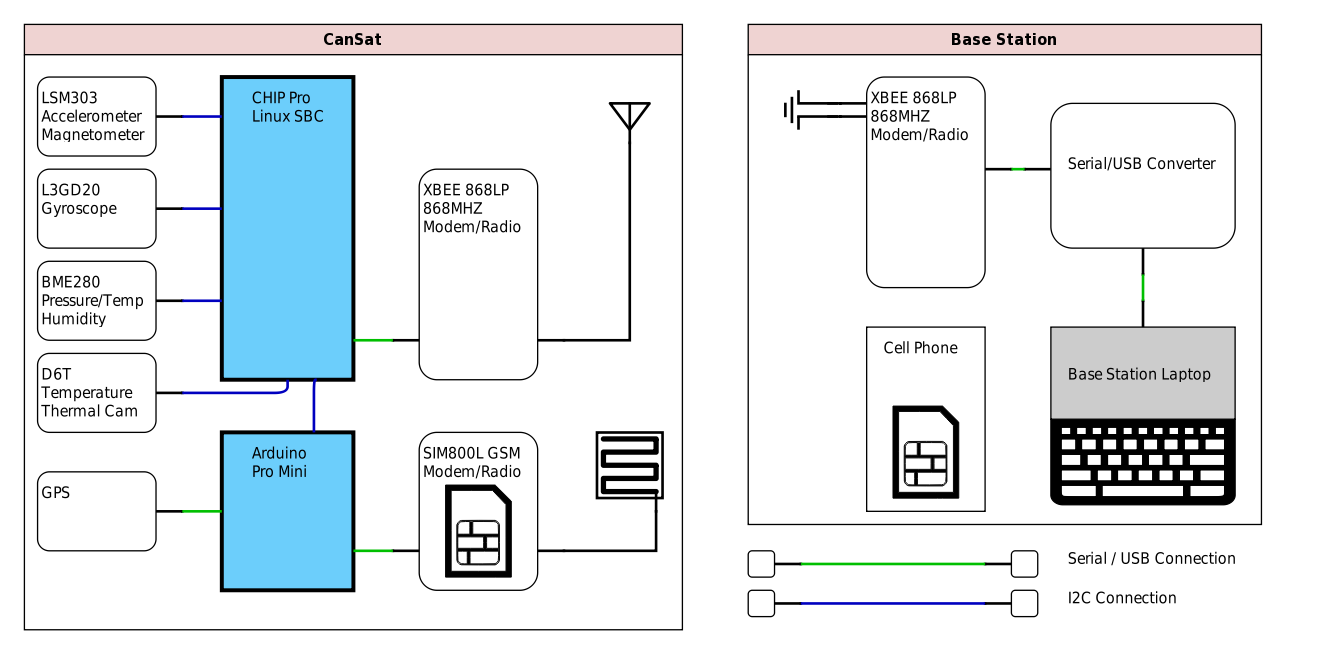
\includegraphics[scale=0.4]{Block_Diagram.png}\hspace*{\fill}
			\caption{CanSat block diagram}
			\label{bdiagram}
		\end{figure}
		
		\section{Prototype CanSat}
		\label{sect:prot}
		While the prototype CanSat maintained a similar sensor and device payload to the final CanSat, it was created via simplified construction techniques: the only automated assembly device used was a laser cutter, and as such the frame, electronics wiring and layout, and overall mechanical design was created by hand. To provide context for this section of the report an image of the prototype CanSat is included in figure \ref{protcanrend}.
		
		\begin{figure}[h]
			\hfill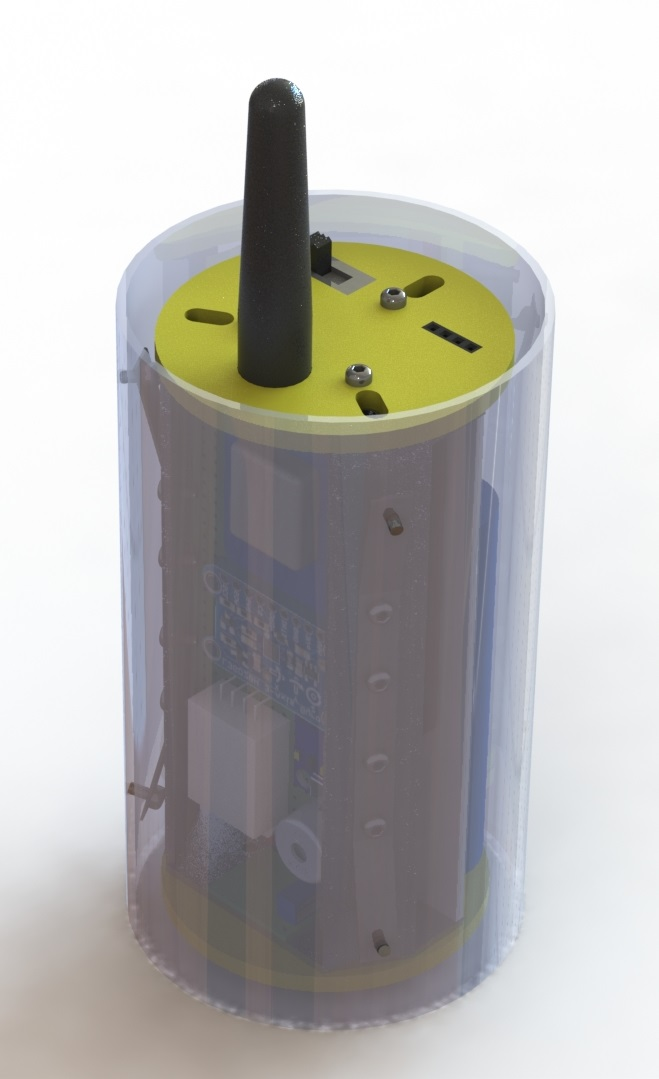
\includegraphics[scale=0.4]{Old_CanSat_render.jpg}\hspace*{\fill}
			\caption{Prototype CanSat Render}
			\label{protcanrend}
		\end{figure}
		
		\subsection{Overview}
		The prototype CanSat is based around the CHIP \footnote{https://getchip.com/} Linux single-board-computer, which runs on a 1GHz Allwinner R8 SoC, 512MB of RAM, and 4GB of Flash, as well as onboard battery regulation and networking. The CanSat also includes an Arduino Pro Mini to allow for serial port expansion and radio redundancy.
		
		In terms of sensor payload, the prototype CanSat includes an IMU \footnote{https://www.adafruit.com/product/1714} containing an LSM303 accelerometer / magnetometer \footnote{https://www.sparkfun.com/datasheets/Sensors/Magneto/LSM303\%20Datasheet.pdf} and an L3GD20 gyroscope \footnote{https://www.pololu.com/file/0J563/L3GD20.pdf}. The prototype CanSat also included a BMP180 pressure / temperature sensor breakout \footnote{https://www.adafruit.com/product/1603}\footnote{https://cdn-shop.adafruit.com/datasheets/BST-BMP180-DS000-09.pdf}, a DHT22 humidity / temperature sensor \footnote{https://www.sparkfun.com/datasheets/Sensors/Temperature/DHT22.pdf}, and a GPS breakout \footnote{https://www.adafruit.com/product/746}.
		
		 A bent aluminum internal frame, with tool assistance given by Heriot Watt \footnote{https://www.hw.ac.uk/index.htm} protects the prototype CanSat, while a fiberglass outer shell serves to absorb shock with its elastic properties.
		 
		 Data transmission is achieved via 2.4GHz radio, and the module is powered by two lithium-ion cells.
		 \subsection{Mechanical Design}
		 \subsubsection{Internal Frame}
		 In order to maximize durability the team decided to split the electronics housing into a tough internal frame and relatively flexible outer shell, attached via a simple mounting mechanism. The goal of this design was for the outer shell to absorb the large forces due to ground collision, while the internal frame provides a structural rigidity and another layer of protection for the sensitive electronics
		 
		 In the development of our internal frame, the team experimented with a variety of materials. As our school stocked 3mm acrylic sheets, we first tested a bent acrylic frame. However, we found that the bend point was lacking the necessary strength for our CanSat, easily shattering on impact. The team then decided to replicate the original design with a bent aluminum frame, seen in figure \ref{intframeold}. 
		 
		 %\begin{wrapfigure}{r}{0.5\textwidth}
		 %	\begin{center}
		 %		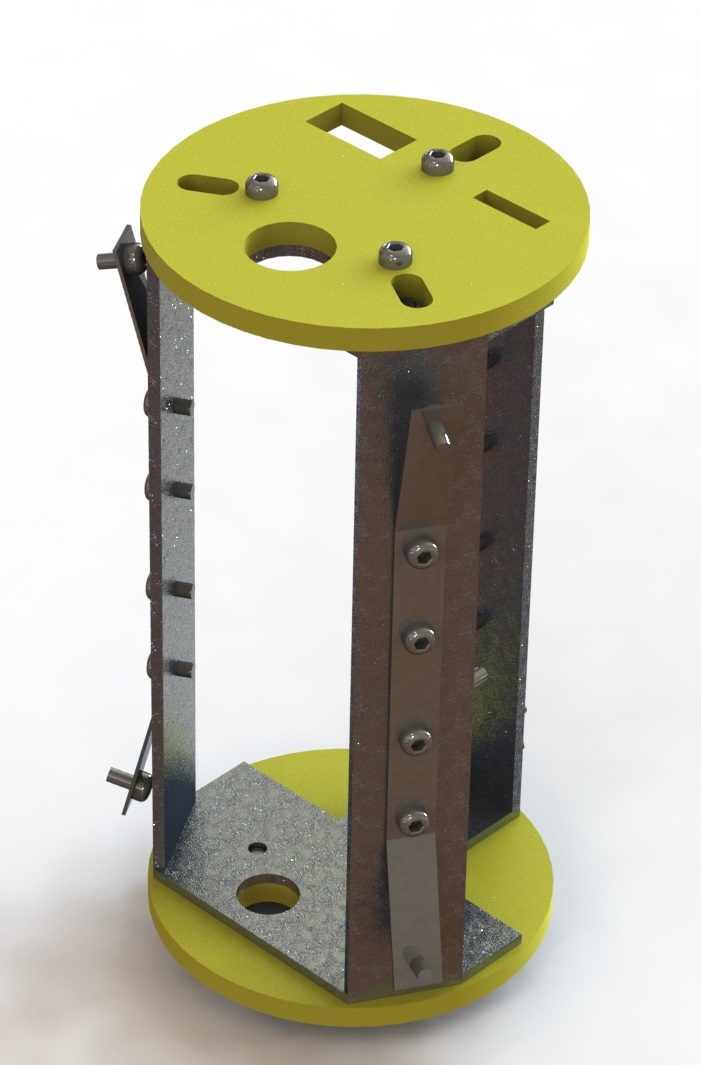
\includegraphics[scale=0.4]{old_int_frame.jpg}
		 %	\end{center}
		 %	\caption{Prototype CanSat internal frame}
		 %	\label{intframeold}
		 %\end{wrapfigure}
		 
		 \begin{figure}[h]
		 	\hfill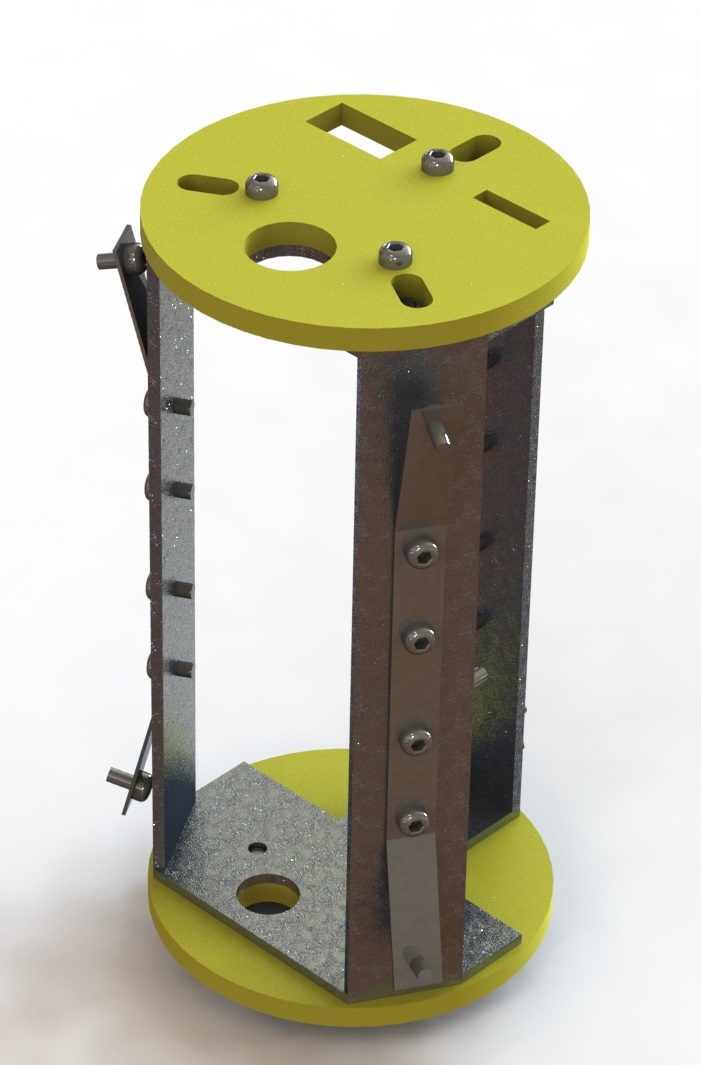
\includegraphics[scale=0.4]{old_int_frame.jpg}\hspace*{\fill}
		 	\caption{Prototype CanSat internal frame}
		 	\label{intframeold}
		 \end{figure}
		 
		 The aluminum frame provided the required rigidity, strength, and toughness for our prototype design. While the internal frame was still relatively basic, lacking specific PCB and sensor mount points, it fulfilled our design requirements.
		 
		 As the team had easy access to a laser cutter via our school, we decided to laser cut top and bottom CanSat plates to provide easy mounting points for antennae, switches, and headers.
		 
		 The development of the CanSat internal frame can be seen via the bottom frames of our prototype CanSat revisions, shown in figure \ref{ointframedev}.
		 
		 
		 \begin{figure}[h]
		 	\hfill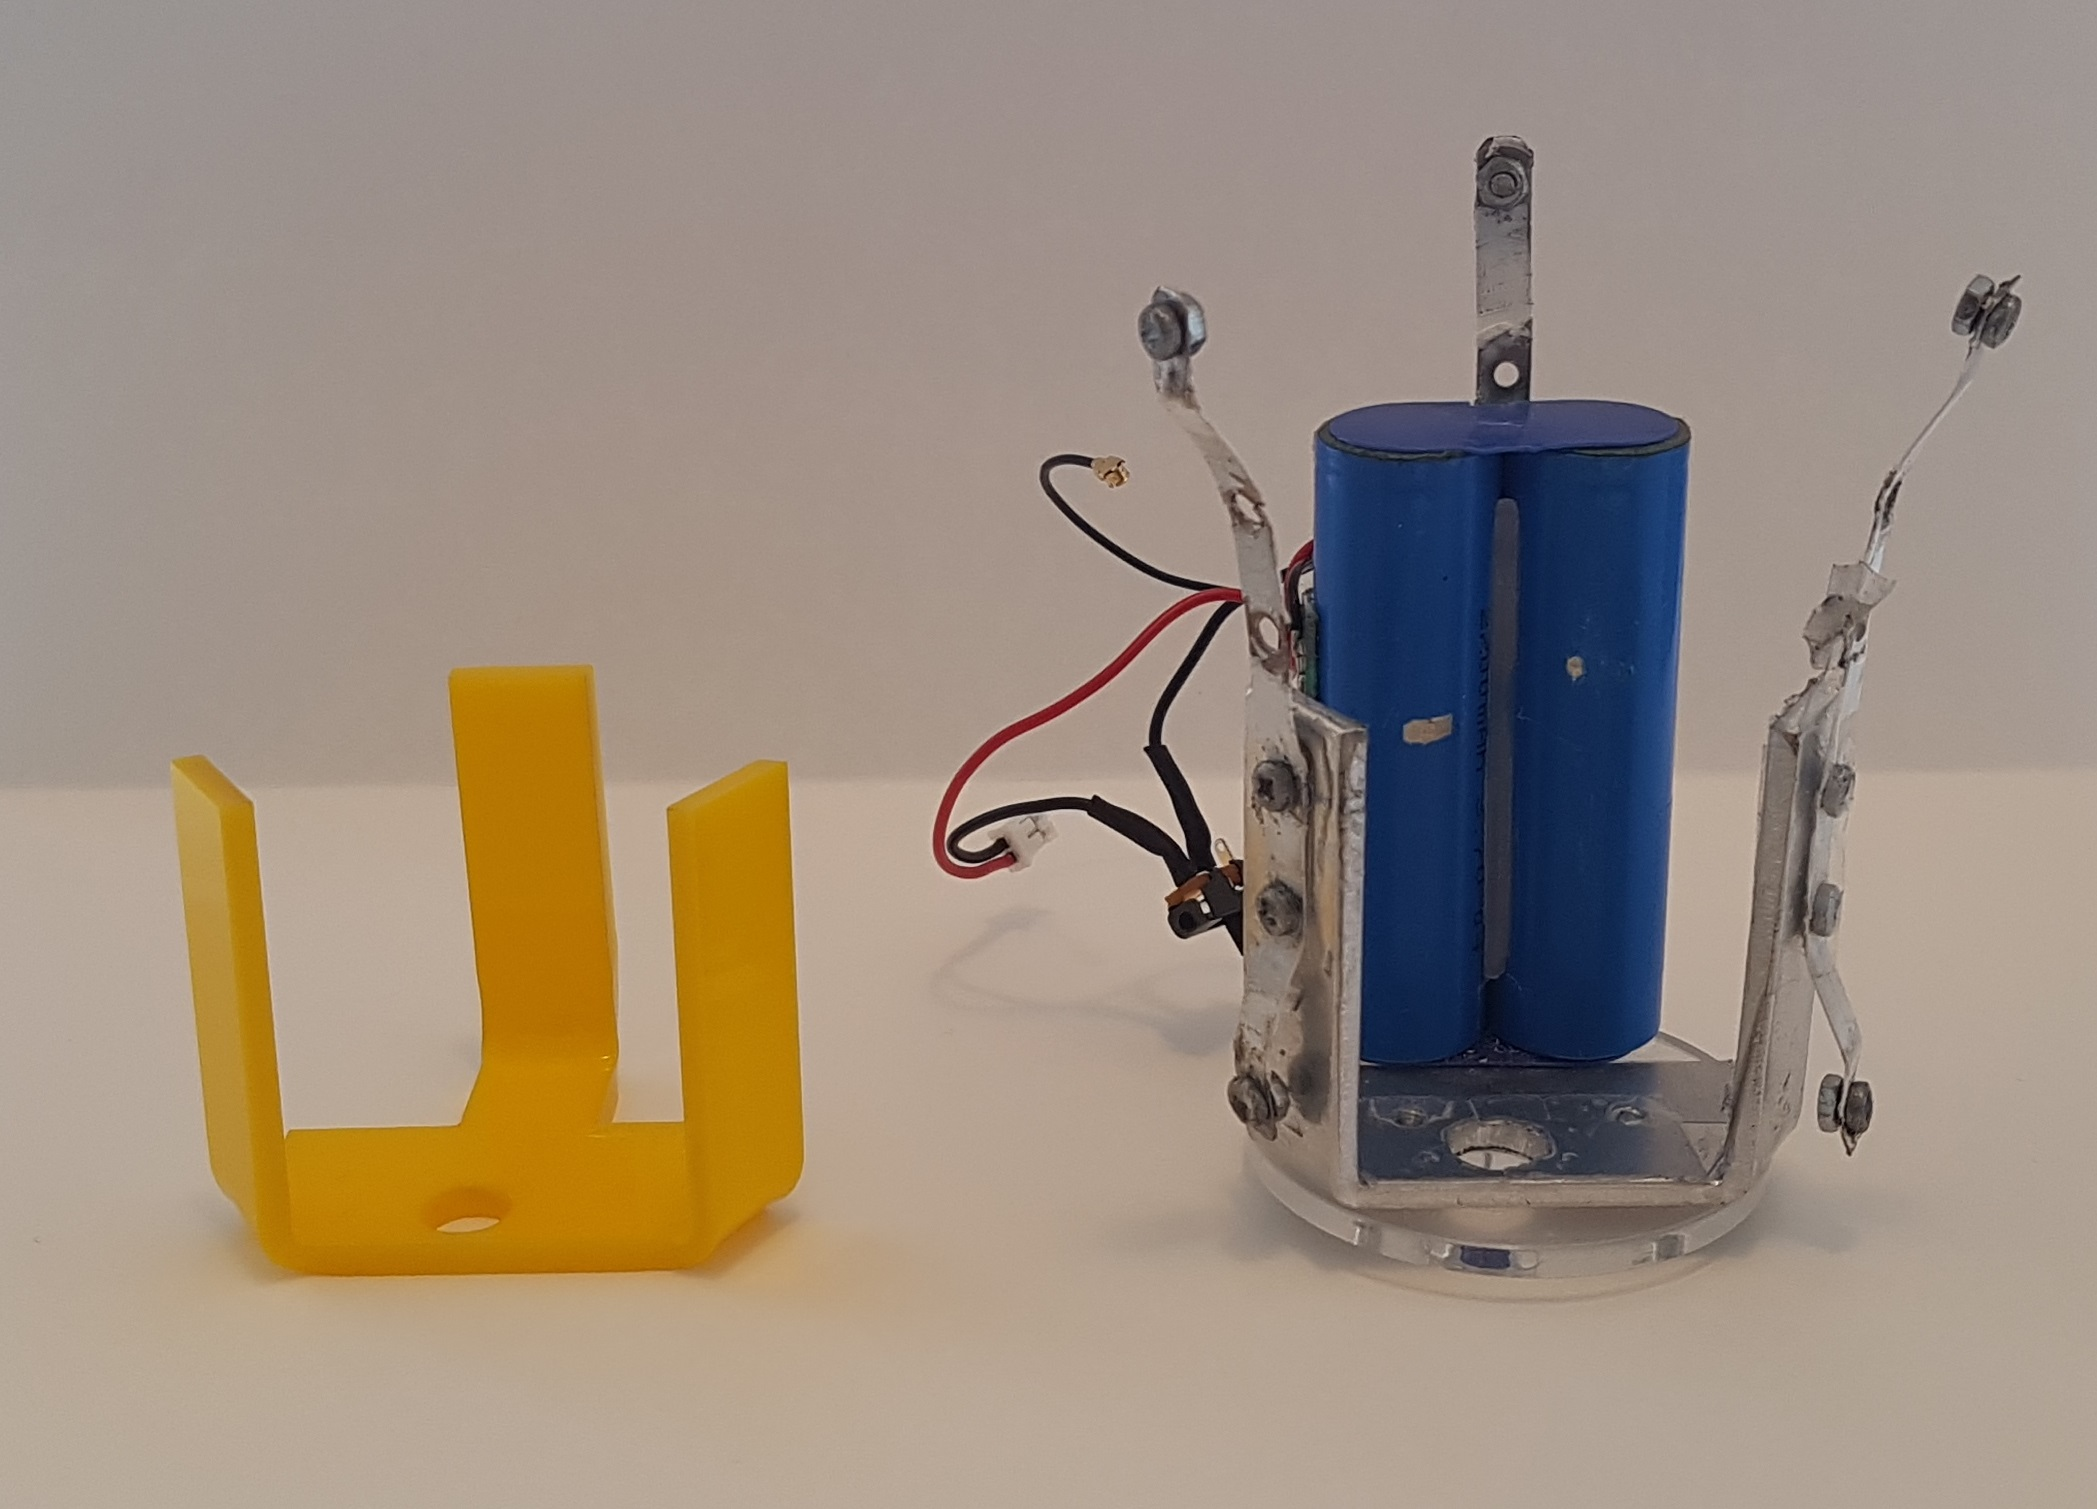
\includegraphics[scale=0.15]{old_frame.jpg}\hspace*{\fill}
		 	\caption{Prototype CanSat internal frame development}
		 	\label{ointframedev}
		 \end{figure}
	 	\subsubsection{Outer Shell}
	 	The team experimented with both 3D printed PLA and fiberglass in the creation of our outer shell. We found PLA to lack strength, easily cracking on impacts, while fiberglass proved to be a difficult material to acquire desired tolerances.
	 	
	 	For our prototype outer shell, the team decided to use fiberglass molded around a bottle of the required diameter. The shell was then cut to size and provided with team and sponsor logos, protected with a transparent plastic sheet. An image of the prototype CanSat and outer shell can be seen in \ref{cshell}. 
	 	
	 	\begin{figure}[h]
	 		\hfill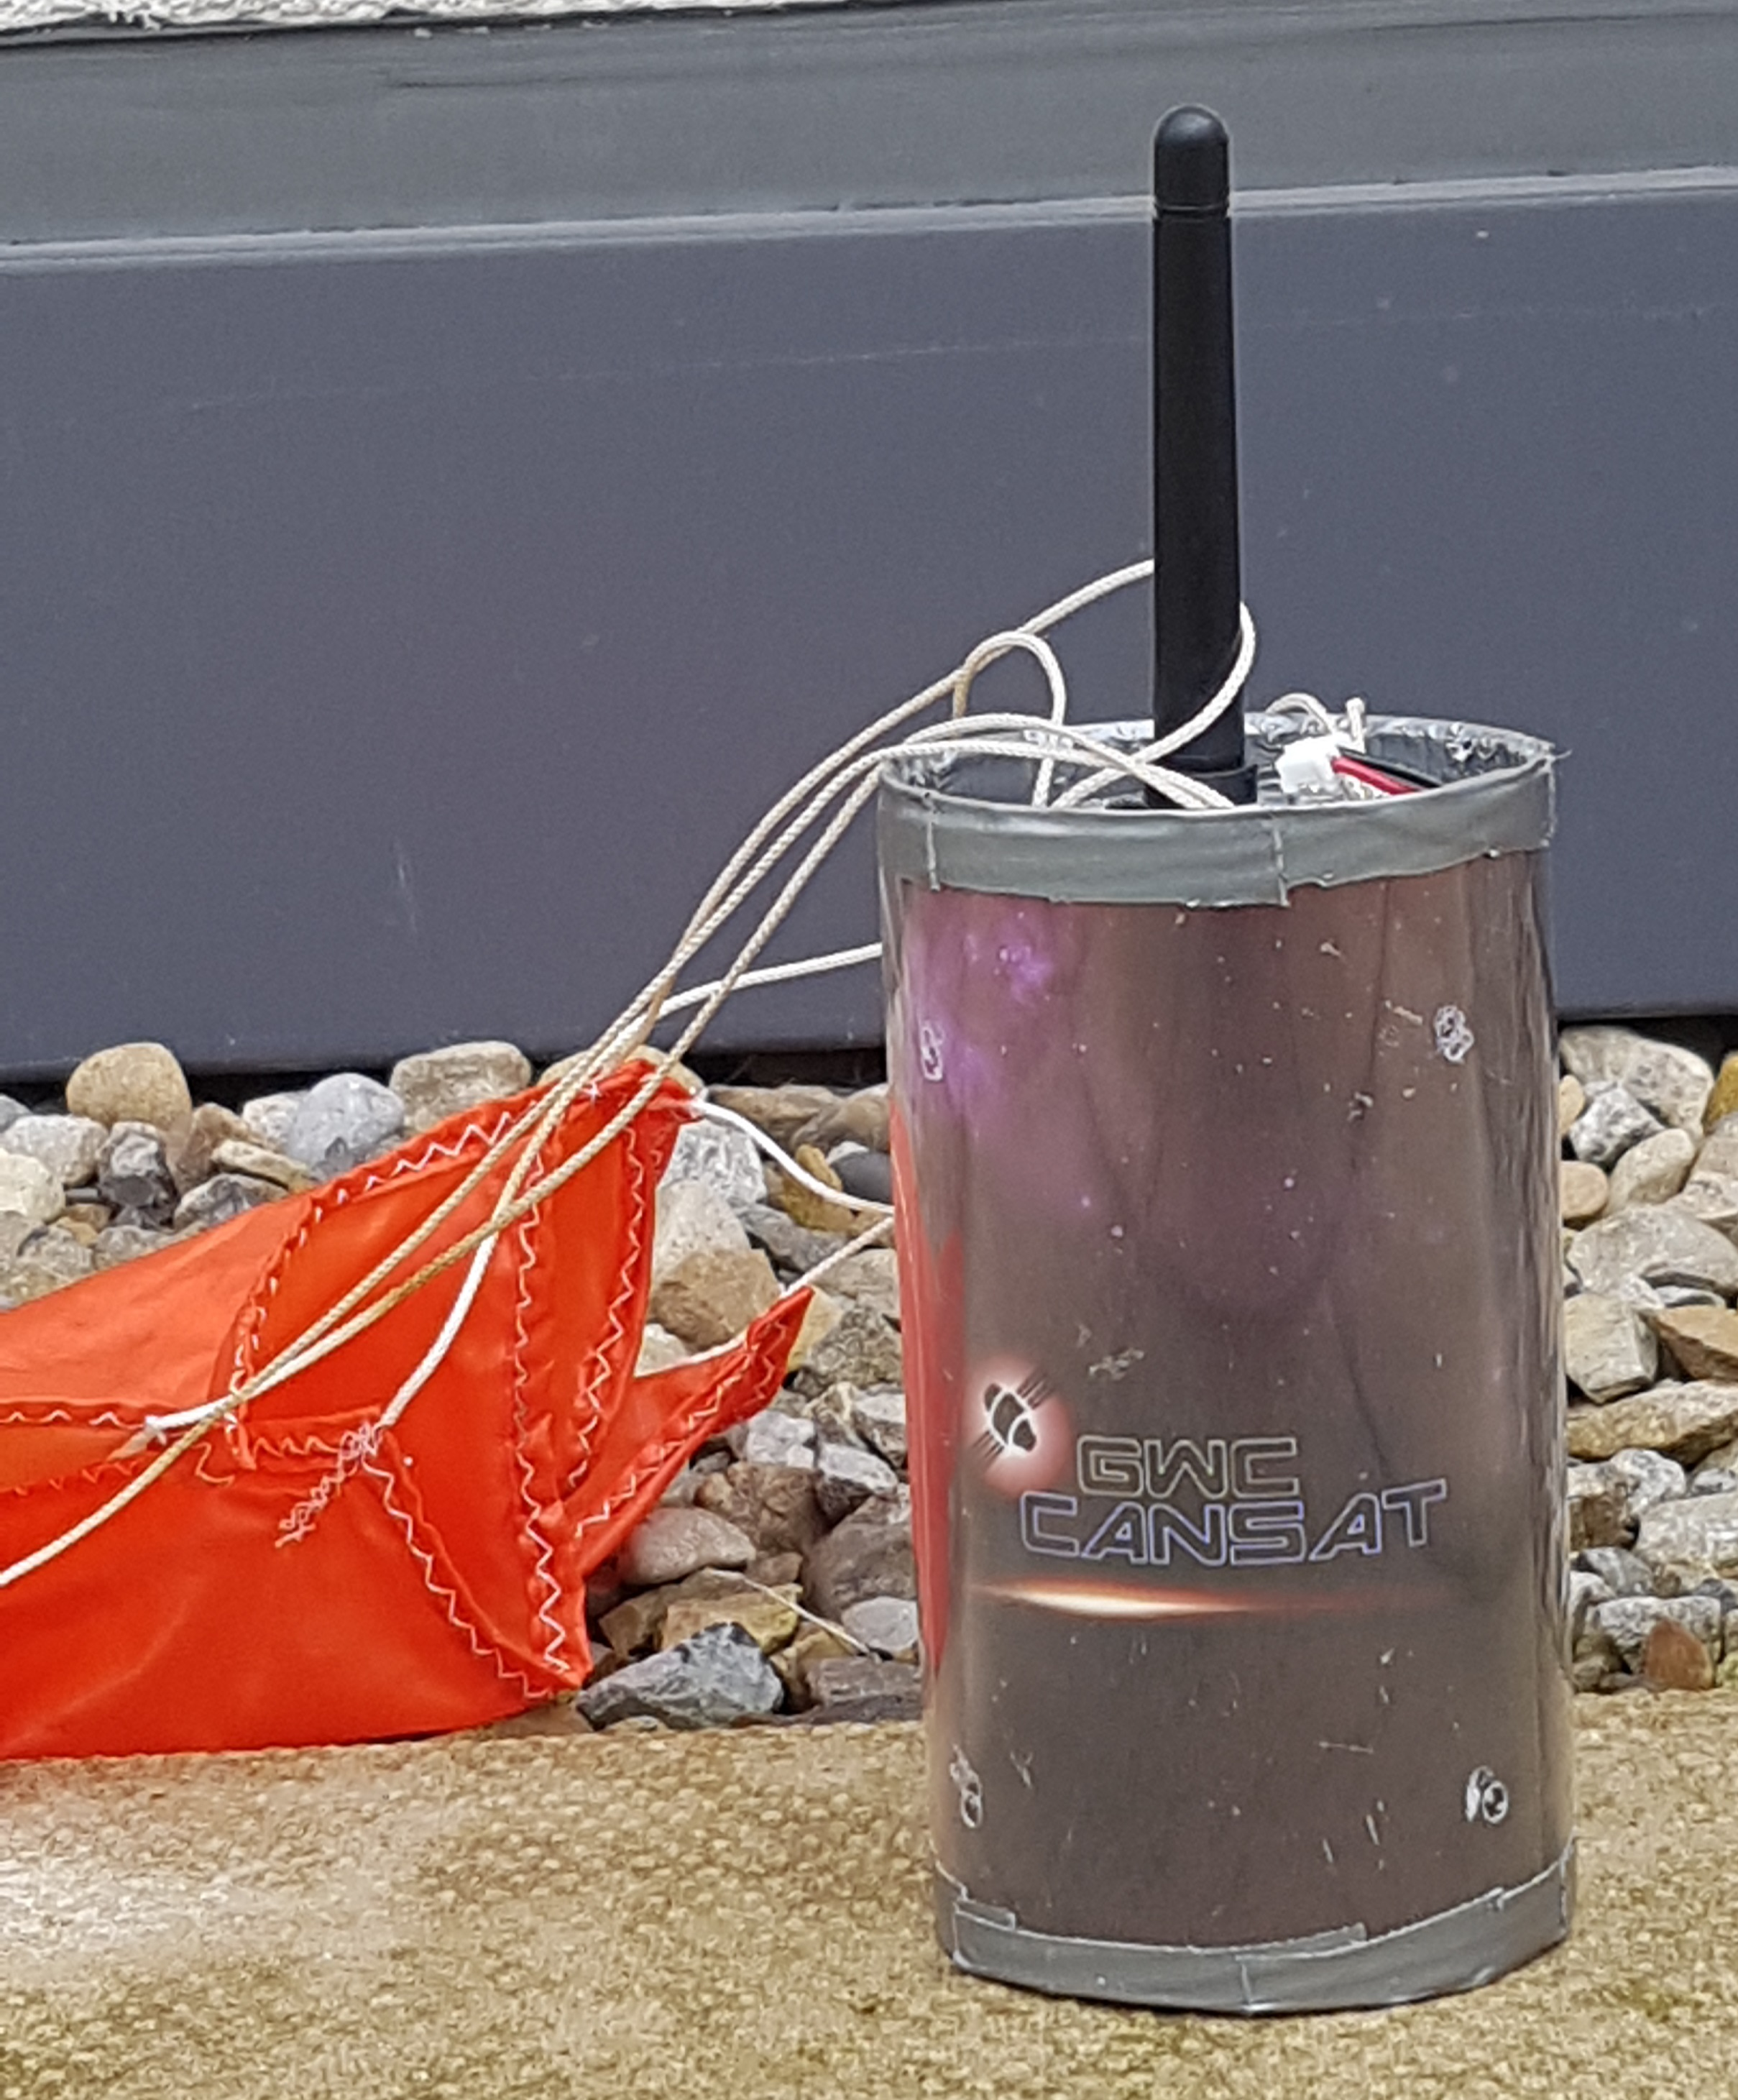
\includegraphics[scale=0.1]{cansat-shell.jpg}\hspace*{\fill}
	 		\caption{The prototype CanSat installed in the outer shell}
	 		\label{cshell}
	 	\end{figure}
	 	
	 	
	 	Spring steel mounts with screw plungers on the internal frame meshed with holes in the outer shell. This design, while offering further shock resistance via the spring steel, created difficulties when removing the internal frame from the outer shell.
	 	\subsubsection{Electronics Mounting}
	 	In the team brainstorming session, we decided to mount all sensors and electronics to a vertical PCB or protoboard. While a set of vertically stacked, circular electronics boards would theoretically provide more surface area, no single board would provide enough space for the single-board-computer and batteries that we aimed to use. Additionally, a single electronics board would facilitate assembly and reduce the number of points of failure. In order to provide long battery runtimes, the team also planned to include a pair of 2200mAh lithium-ion cells in the 18650 form factor \footnote{https://www.adafruit.com/product/354}. The relatively large size of these cells led to a press-fit mount as seen in figure \ref{emount}.
	 	
	 	\begin{figure}[h]
	 		\hfill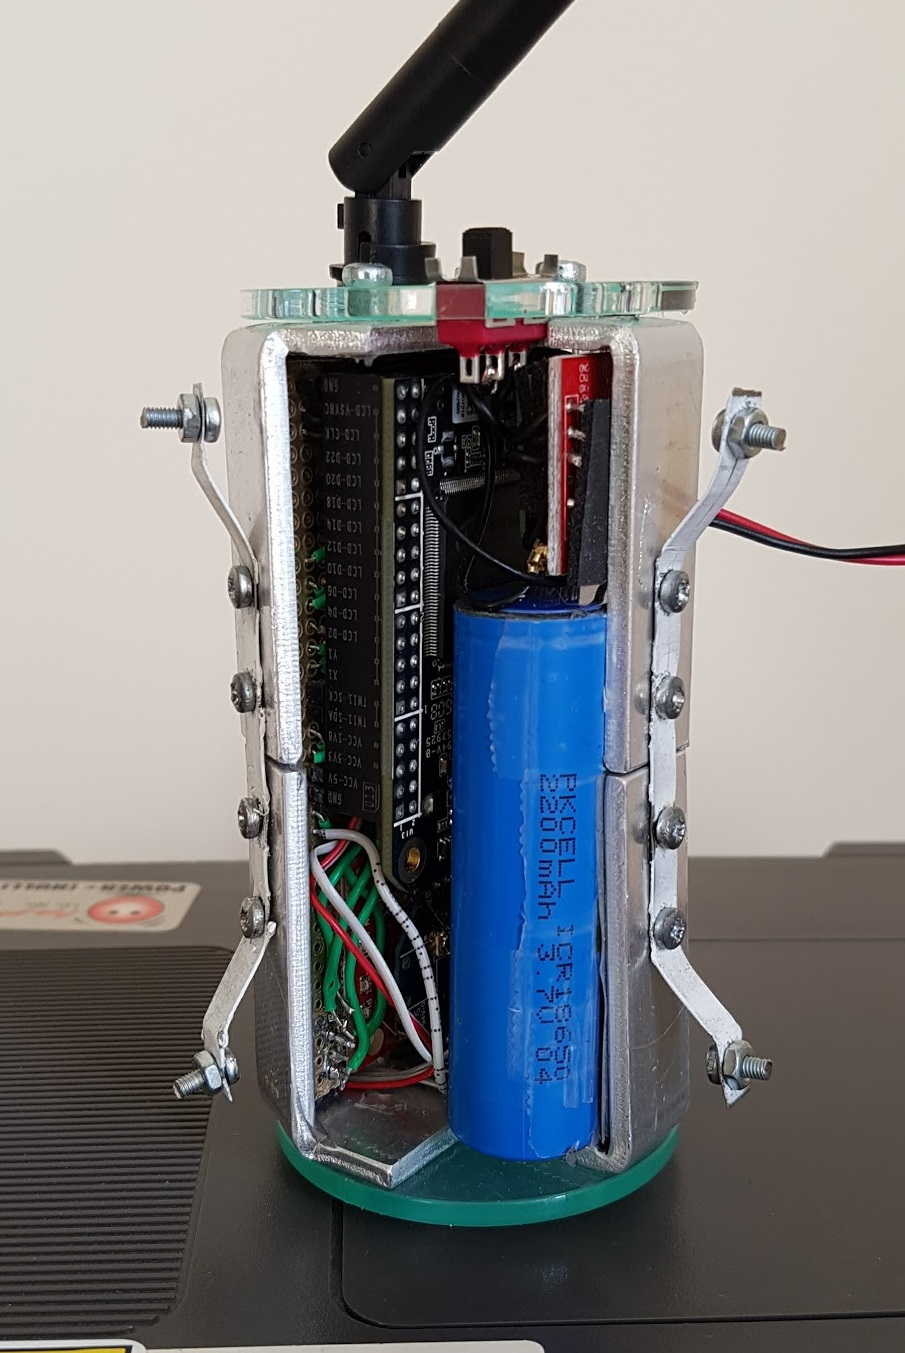
\includegraphics[scale=0.4]{old_cansat_side.jpg}\hspace*{\fill}
	 		\caption{Electronics mount on the prototype CanSat}
	 		\label{emount}
	 	\end{figure}
	 	
	 	The thermal camera was placed at the bottom of the CanSat, against the steel frame, and the cellular GSM module was secured via adhesive above the battery. An annotated image of the prototype CanSat can be seen in figure \ref{anoldcan}.
	 	
	 	\begin{figure}[h]
	 		\hfill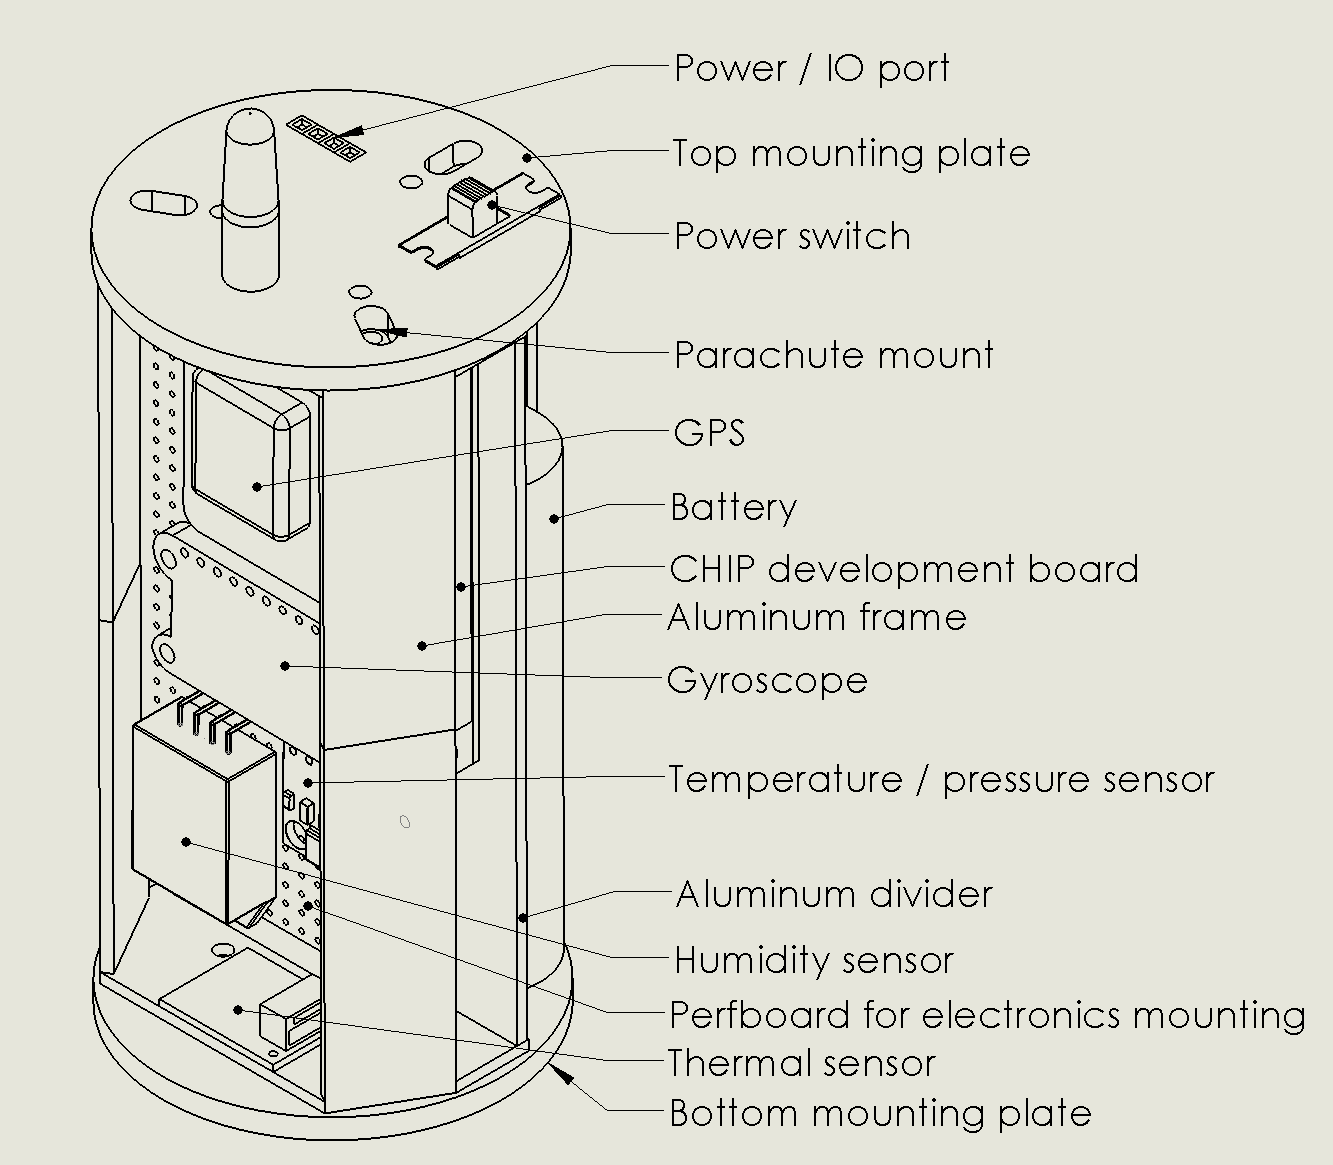
\includegraphics[scale=0.2]{annotated_cansat.png}\hspace*{\fill}
	 		\caption{An annotated view of the prototype CanSat}
	 		\label{anoldcan}
	 	\end{figure}
 		\subsection{Electrical Design}
 		\subsubsection{Sensor and Device Wiring}
 		Similar to the section describing the mechanical design, the team's experiences in our prototyping phase provide context to our design decisions in our final CanSat design.
 		
 		Throughout our CanSat brainstorming, prototyping, and final design, the team used a Linux single-board-computer as the main control board in our CanSat. One of our team's objectives was for the CanSat to stay relatively independent of the base station- to be able to do all sensor processing on-CanSat, to compensate for any electrical, radio, or hardware failures, and, if necessary, for the base station to be able to alter CanSat code over a radio connection. These objectives required more computing power than was available in the eight-bit Atmel MCUs common in hobby development boards, so the team settled on a Linux SBC: the CHIP, designed by Next Thing Co, for our prototype design. The CHIP includes a 1GHz ARM CPU, 4GB of Flash, and 512MB of RAM. For this design, sensor payload was as seen in figure \ref{anoldcan}: 
 		
 		The CHIP provided battery regulation and charging, as well as stable and high-current-capable 5V, 3.3V, and 1.8V rails. We experienced no issues powering sensors and radios, though logic level shifting circuitry was necessary for some sensors.
 		
 		The team did struggle with serial I/O in our prototype design. The CHIP theoretically supports multiple serial ports, but the team was only able to interface with one port echoing the Linux console. Hence we added an Arduino Pro Mini to serve as a serial-I2C interpreter. 
 		
 		Our prototype design saw these components wired to a single protoboard as seen in figure \ref{pboard}.
 		
 		\begin{figure}[h]
 			\hfill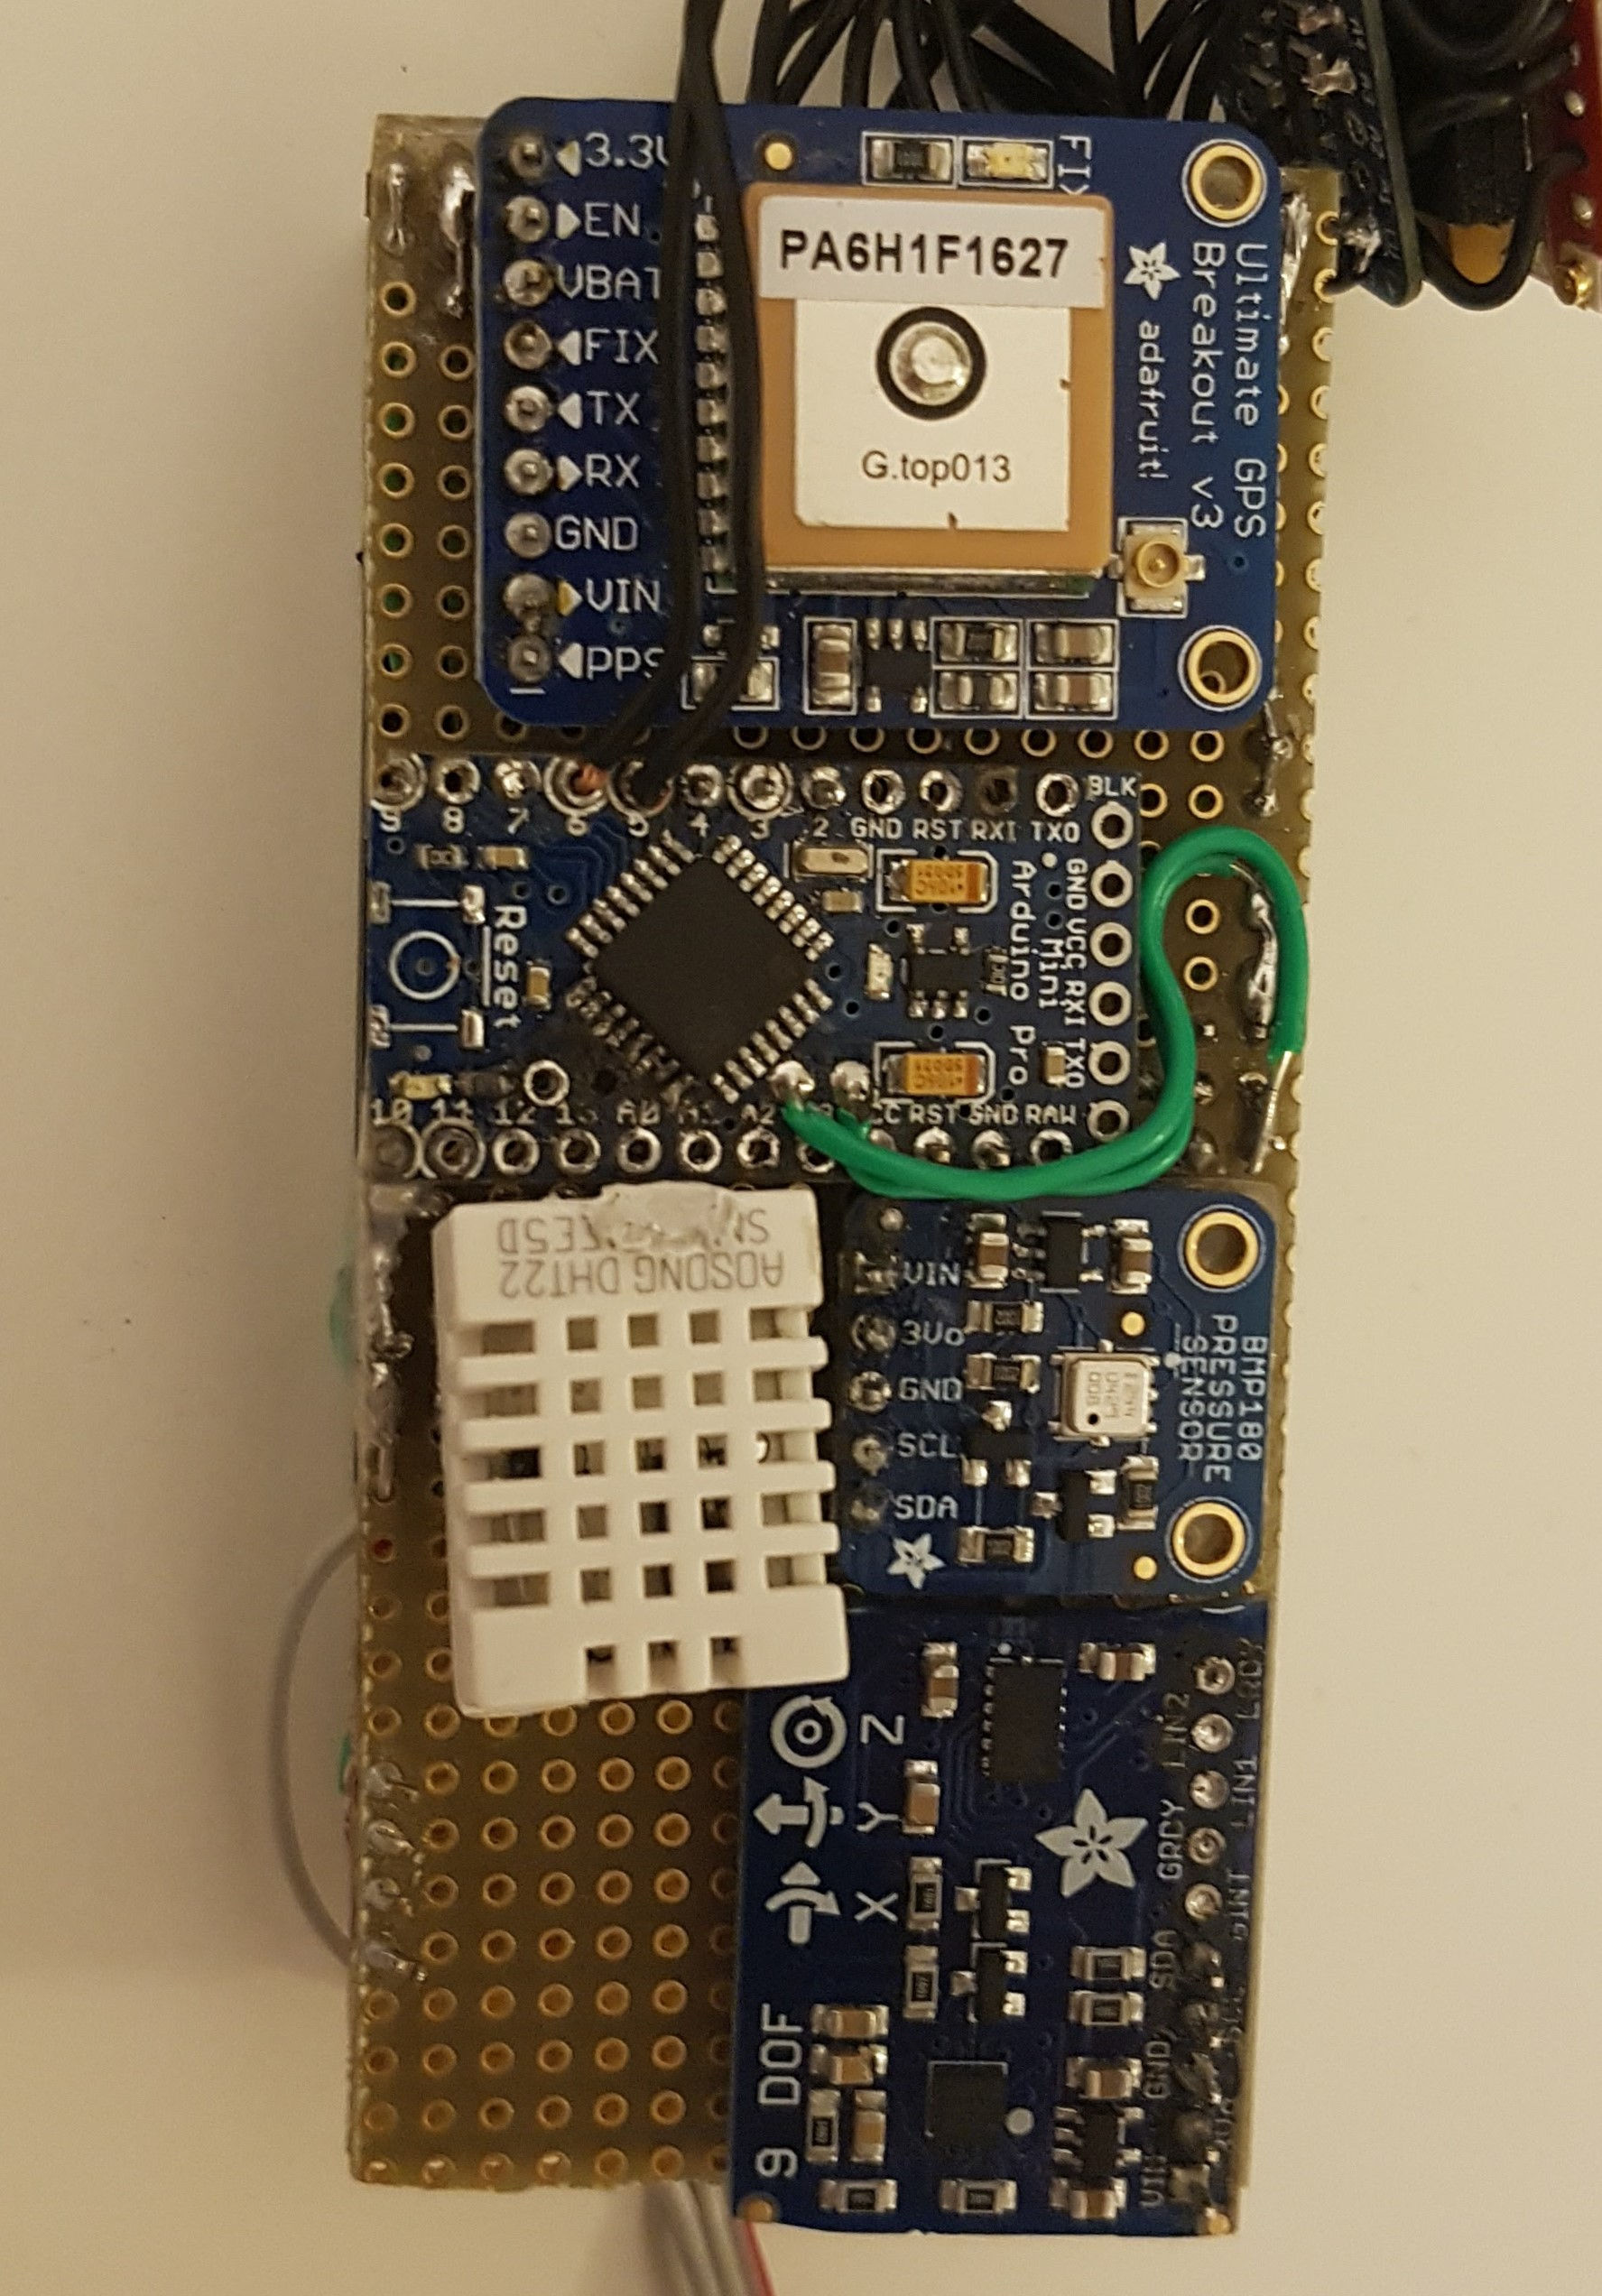
\includegraphics[scale=0.1]{protoboard.jpg}\hspace*{\fill}
 			\caption{The prototype CanSat electronics board}
 			\label{pboard}
 		\end{figure}
 		\subsubsection{Radio Specifications}
 		Our prototype design included two radios: an XBEE Pro 2.4GHz \footnote{https://www.sparkfun.com/products/8710} and a SIM800L GSM module \footnote{http://www.datasheetspdf.com/datasheet/SIM800L.html}. This dual radio design, as seen in the schematic in figure \ref{cschem}, provides redundancy and assists emergency recovery of the CanSat. If the primary radio link is lost, or CHIP failure is experienced, the CanSat GPS coordinates will be sent via SMS to a team member's cell phone. 
 		
 		The XBEE Pro is a simple all-in-one radio and modem module allowing for long range encrypted communication over the 802.15.4 Zigbee protocol. At peak bandwidth, the modules are capable of a 250kbps transmit rate in either point to point or multi-point networks. The XBEE Pro consumes 215mA during data transmit and has a maximum range of 1.5km.
 		
 		The team decided to use the XBEE module due to these features. The Zigbee protocol is widely used, making our CanSat compatible with thousands of data logging devices already in use, and the module's integrated spread-spectrum technology allows for reliable long-range communication in heavy interference. Finally, the modules can allow a transparent serial link between the CanSat and base station: the base station can access the CHIP Linux terminal with packetization handled onboard the XBEE. 
 		
 		The SIM800L was chosen due to its cost, ubiquity, and large feature set. At USD 6.99 per unit including a breakout board, the module was easy to fit in our CanSat budget. Additionally, the SIM800L provides easy configuration via the well-documented AT command set. The SIM800L consumes approximately 40mA in receive mode, with millisecond spikes of up to 2A while transmitting.
 		\subsubsection{Battery Specifications and Estimated Runtime}
 		Our battery choice has remained constant through our prototype and final designs, with a pair of 2200mAh lithium ion cells connected via a load balancer \footnote{https://www.adafruit.com/product/354}.
 		
 		There are many downsides associated with the use of lithium-ion cells. Their high energy density can lead to thermal runaway and combustion, damaging the CanSat, and battery performance suffers in cold temperatures. However, it is important to note that the CanSat will be dropped from a height of 1km: too low to see any major temperature delta. Additionally, our prototype CanSat has shown that the outer shell and internal frame provide enough support to protect the batteries. The team has also decided to include foam padding at the bottom of the battery compartment to further prevent damage.
 		
 		CanSat power usage and estimated runtime:
 		
 		\begin{center}
 			\begin{tabular}{ll}
 				Sensor&Power Consumption\\
 				\hline
 				GPS&20mA \\
 				MEMS sensors&10mA total \\
 				CHIP Pro&270mA mean \\
 				Arduino Pro Mini&15mA \\
 				SIM800L&40mA \\
 				XBEE 868LP&48mA \\
 				Power Supply inefficiency&50mA approx\\
 				\hline
 				Total&413mA
 			\end{tabular}	
 		\end{center}	
 		
 		With a 4400mAh battery, this leads to a calculated runtime of $\frac{4400}{413}=10.65$ hours. However, this calculation assumes that the CanSat is constantly transmitting: in real-world tests, the CanSat does not constantly transmit and hence reaches runtimes of between 12 and 13 hours.
 		
 		\subsection{Software Design}
 		\subsubsection{On-CanSat Software}
 		The prototype CanSat's software is divided into two parts: a python script running onboard the CHIP, and an Arduino script providing serial expansion and DHT22 humidity sensor parsing. Both sections of our CanSat software are available on the team GitHub \footnote{https://github.com/Arcturus314/cansat2017} under the "ukcode" directory.
 		
 		The CHIP script is relatively simple. It uses premade I2C sensor drivers to fetch data from our various sensors, collates this data into a list, logs it in a text file, and transmits it back to the base station. It then awaits a response from the base station, which indicates whether to wipe CanSat data files, disable sensors, or perform other commands. When this packet is received, parsed, and executed, another data packet is sent from the CanSat to the base station. Base station communication is handled in a separate thread from sensor logging: hence data will still be logged if a radio connection is lost.
 		
 		The Arduino script is similarly simple. It uses an Adafruit library \footnote{https://github.com/adafruit/DHT-sensor-library} to interact via the DHT22 one-wire interface, logs data from the GPS \footnote{https://github.com/adafruit/Adafruit\_GPS}, and supports SIM800L interaction. This data is sent to the CHIP via a similar list-based mechanism, and the script also supports return packets for sensor and SIM800L control. One of the major issues with this system is that the list-based format did not include packet header and footer markers: hence the Arduino and CHIP could become "out-of-sync" if a character is not properly transmitted through the I2C bus, leading to the loss of all Arduino data until a reboot.
 		
 		\subsubsection{Base Station Software}
 		The base station served as a control interface and GUI for visualizing received CanSat data. It allowed for both control over the Cansat data lists and independent logging of any received data. It was written in python, with MatPlotLib \footnote{https://matplotlib.org/} used for all GUI and graphing work, and pySerial \footnote{https://pythonhosted.org/pyserial/} used to provide a serial interface with the base station XBEE radio module. 	
 		
 		An image of the base station in operation can be seen in figure \ref{oldgui}.	
 		
		\begin{figure}[h]
			\hfill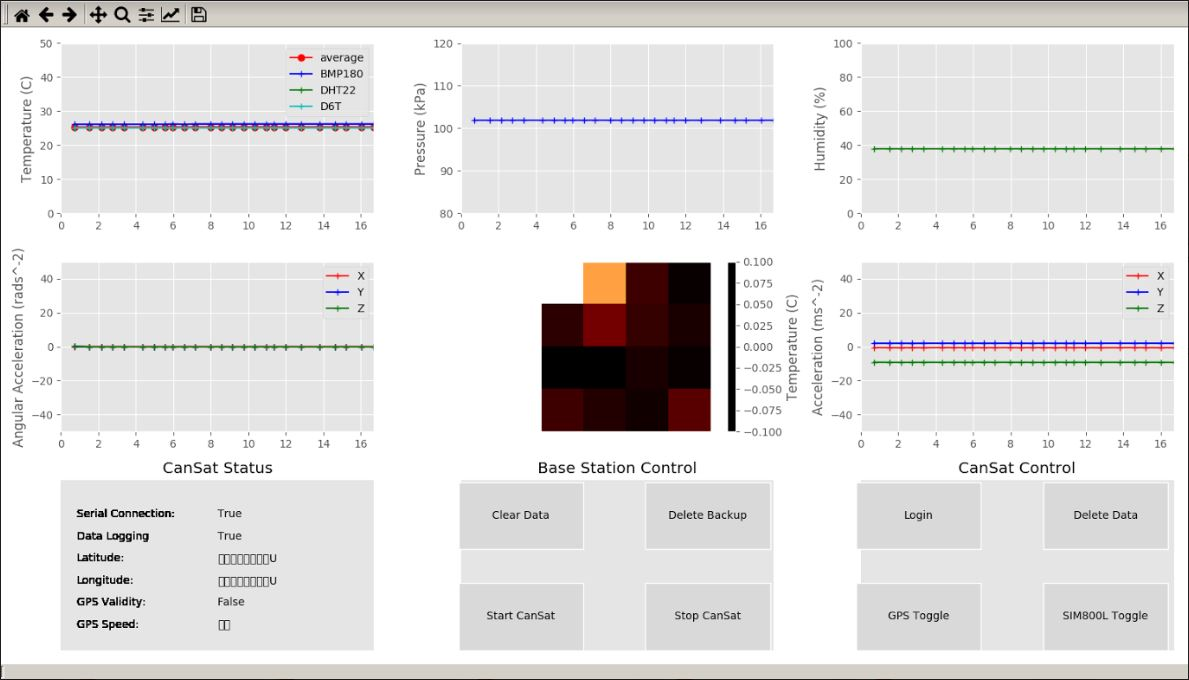
\includegraphics[scale=0.4]{old_gui.jpg}\hspace*{\fill}
				\caption{The UK Competition CanSat GUI without a GPS lock}
			\label{oldgui}
		\end{figure}
	
		\subsection{Budget}
		
		The prototype CanSat budget is described below:
		
		\begin{center}
			\begin{longtable}{llll}
				Component Name                 & Unit Price (USD) & Total Price (USD) & Price (EUR) \\ \hline
				Perfboard                      & 11.82            & 11.82             & 10.4016     \\
				CHIP                           & 9                & 9                 & 7.92        \\
				XBEE Explorer Regulated        & 9.95             & 9.95              & 8.756       \\
				XBEE Pro 60mW                  & 37.95            & 37.95             & 33.396      \\
				Omron D6T                      & 42.9             & 42.9              & 37.752      \\
				Adafruit BMP180                & 9.95             & 9.95              & 8.756       \\
				Adafruit Ultimate GPS          & 39.95            & 39.95             & 35.156      \\
				Adafruit DHT22                 & 9.95             & 9.95              & 8.756       \\
				Adafruit 9DOF                  & 19.95            & 19.95             & 17.556      \\
				Digi 2.4GHz Antenna            & 4.94             & 4.94              & 4.3472      \\
				Slide Switch                   & 2.27             & 2.27              & 1.9976      \\
				Female 5x1 Header              & 0.81             & 0.81              & 0.7128      \\
				Thermal Sensor Contact         & 0.11             & 0.44              & 0.3872      \\
				Thermal Sensor Housing         & 0.13             & 0.13              & 0.1144      \\
				Spring Steel Boning Stays      & 2.75             & 2.75              & 2.42        \\
				GSM Module                     & 6.18             & 6.18              & 5.4384      \\
				Adafruit Logic Level Converter & 3.95             & 3.95              & 3.476       \\
				Parachute                      & 7.37             & 7.37              & 6.4856      \\
				Wire (assorted)                & 5                & 5                 & 4.4         \\
				Aluminum (assorted)            & 5                & 5                 & 4.4         \\
				Fibreglass                     & 10               & 10                & 8.8         \\ \hline
				Sum:                           &                  & 240.26            & 211.4288   
		\end{longtable}
	\end{center}
			 
		 
	\section{Final CanSat}
		\label{sect:final}
		
		\subsection{Overview}
		Through our design revisions to the final CanSat, we have been able to utilize more sponsors and funding to create a far refined version of our prototype CanSat- it has been improved in almost every way, from custom designed PCBs, to composite metal and plastic internal frames, to more accurate sensors and longer range radios. To clarify the next few sections images of the final CanSat are shown below:
		
		\begin{figure}
			\centering
			\begin{subfigure}{.5\textwidth}
				\centering
				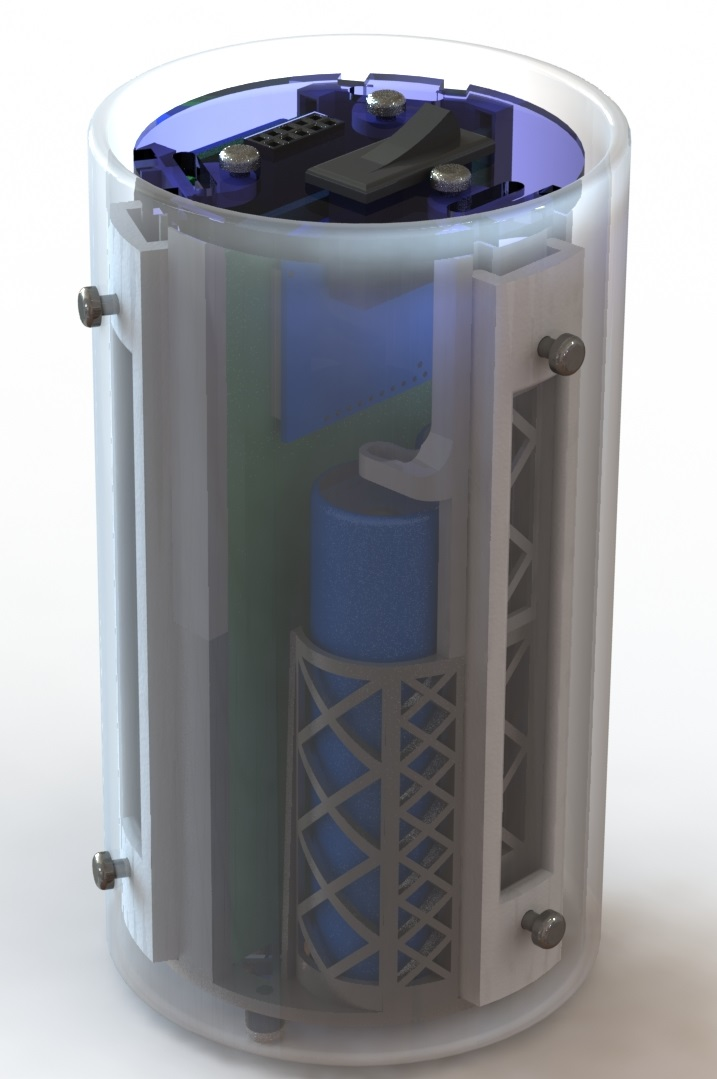
\includegraphics[width=.8\linewidth]{CanSat_render.jpg}
			\end{subfigure}%
			\begin{subfigure}{.5\textwidth}
				\centering
				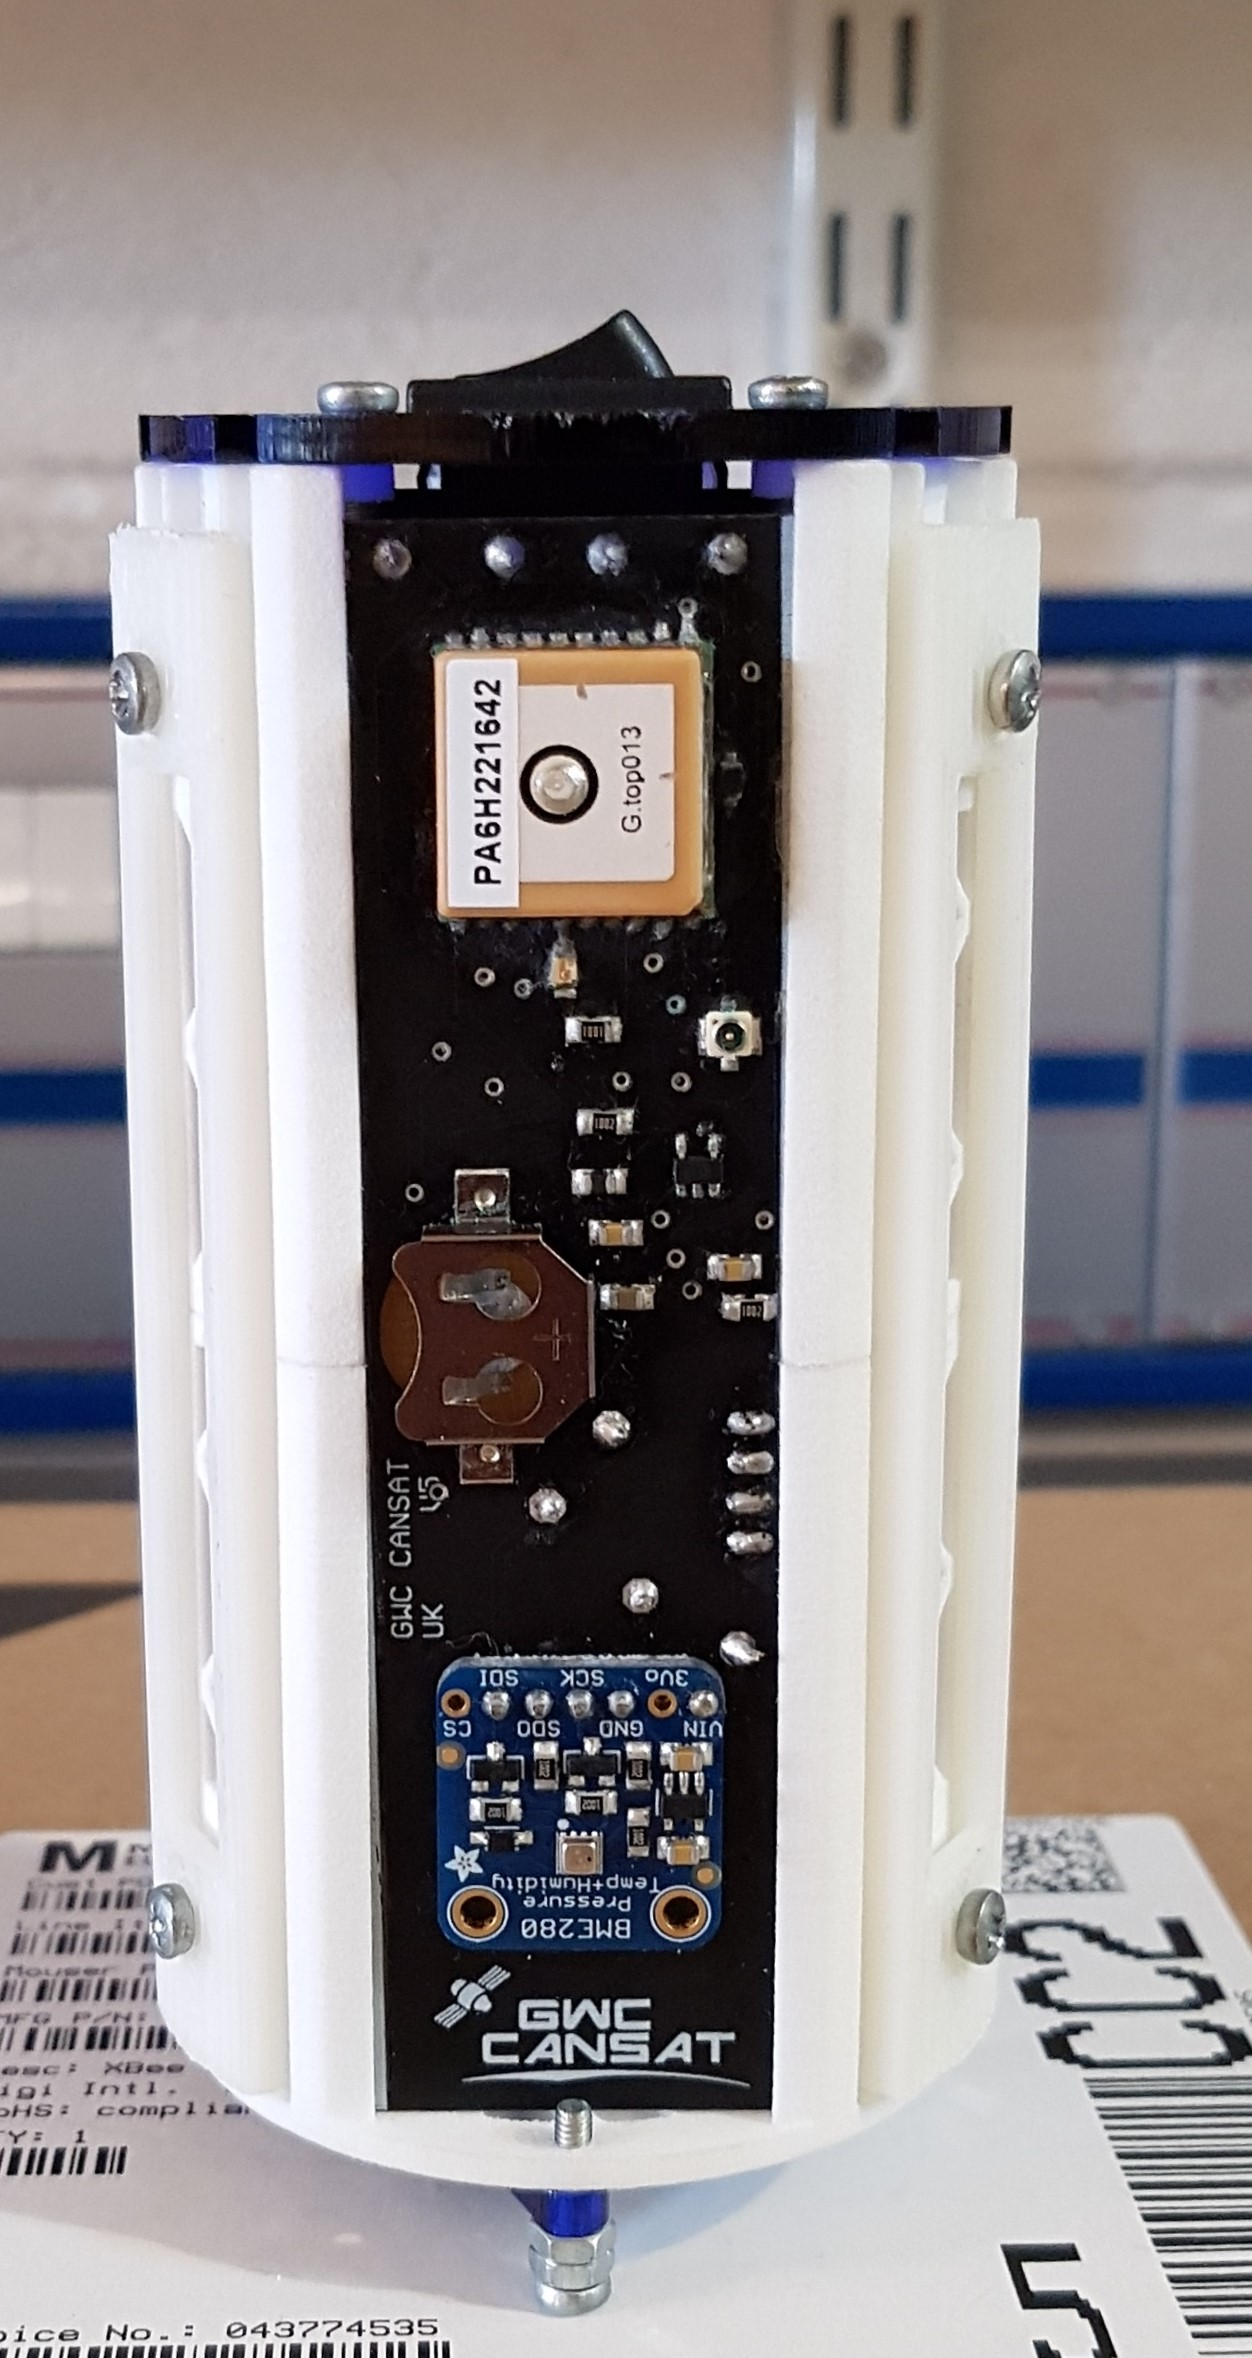
\includegraphics[width=0.6\linewidth]{new_cansat.jpg}
			\end{subfigure}
			\caption{Final CanSat design}
			\label{newcansat}
		\end{figure}
		
		\subsection{Mechanical Design}
		
		\subsubsection{Internal Frame}
		
		In the team's second design revision, we aimed to use additive manufacturing to allow for a more complex internal frame, maximizing strength, minimizing weight, and allowing for sensor, PCB, and battery mounting points directly on the internal frame, as illustrated in figure \ref{newframerender}.
		
		%\begin{wrapfigure}{L}{0.5\textwidth}
		%	\begin{center}
		%		\includegraphics[scale=0.4]{cansat_internal_frame_render.jpg}
		%	\end{center}
		%	\caption{Final CanSat internal frame render}
		%	\label{newframerender}
		%\end{wrapfigure}
		
		\begin{figure}[h]
			\hfill\includegraphics[scale=0.4]{cansat_internal_frame_render.jpg}\hspace*{\fill}
			\caption{Final CanSat internal frame render}
			\label{newframerender}
		\end{figure}
		
		We again elected to split the CanSat frame into top and bottom components. The top frame was composed of three discrete vertical support bars, providing slider trenches and screw holes for mounting the outer shell, slots for mounting PCBs, as well as battery-holding prongs and parachute/top plate mounting points. These support bars were attached via a laser-cut top plate, again providing switch and header mounting points, as well as holes to allow for parachute mounts- this is shown in figure \ref{topframerender}.
		
		%\begin{wrapfigure}{R}{0.5\textwidth}
		%	\begin{center}
		%		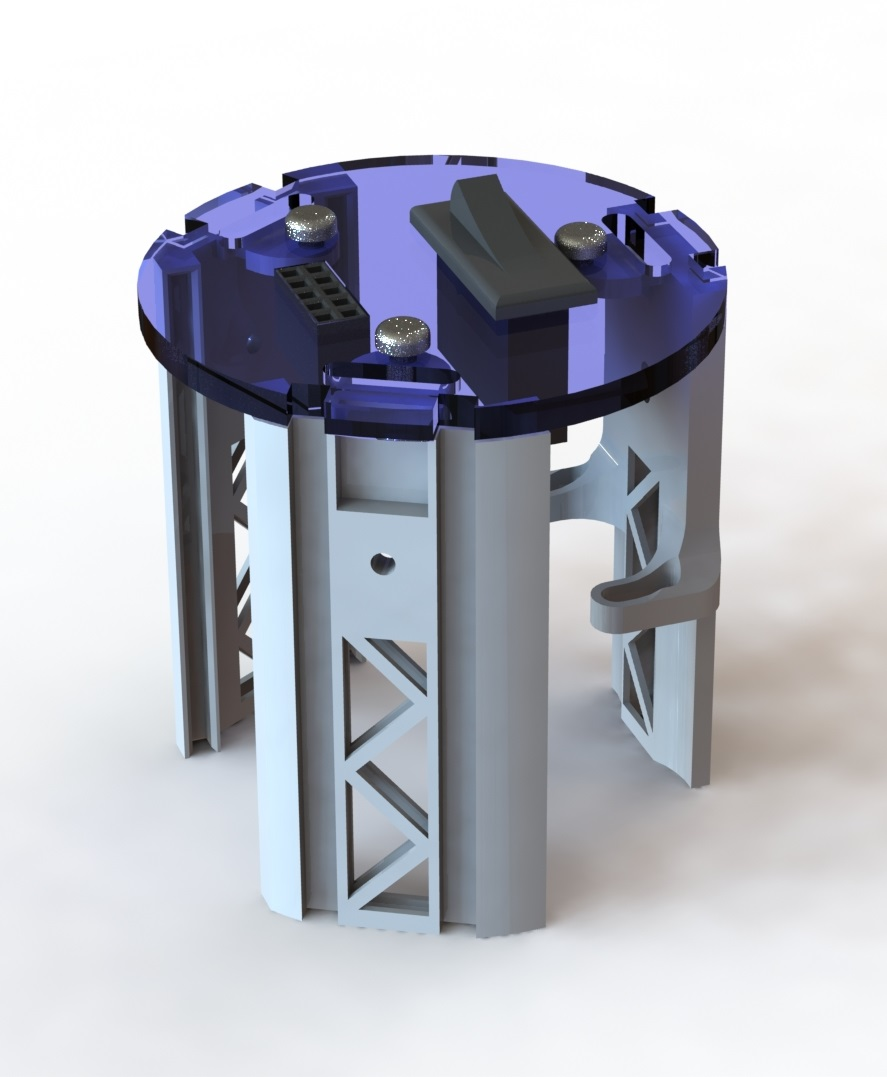
\includegraphics[scale=0.4]{Top_frame_render.jpg}
		%	\end{center}
		%	\caption{Final CanSat top frame render}
		%	\label{topframerender}
		%\end{wrapfigure}
		
		\begin{figure}[h]
			\hfill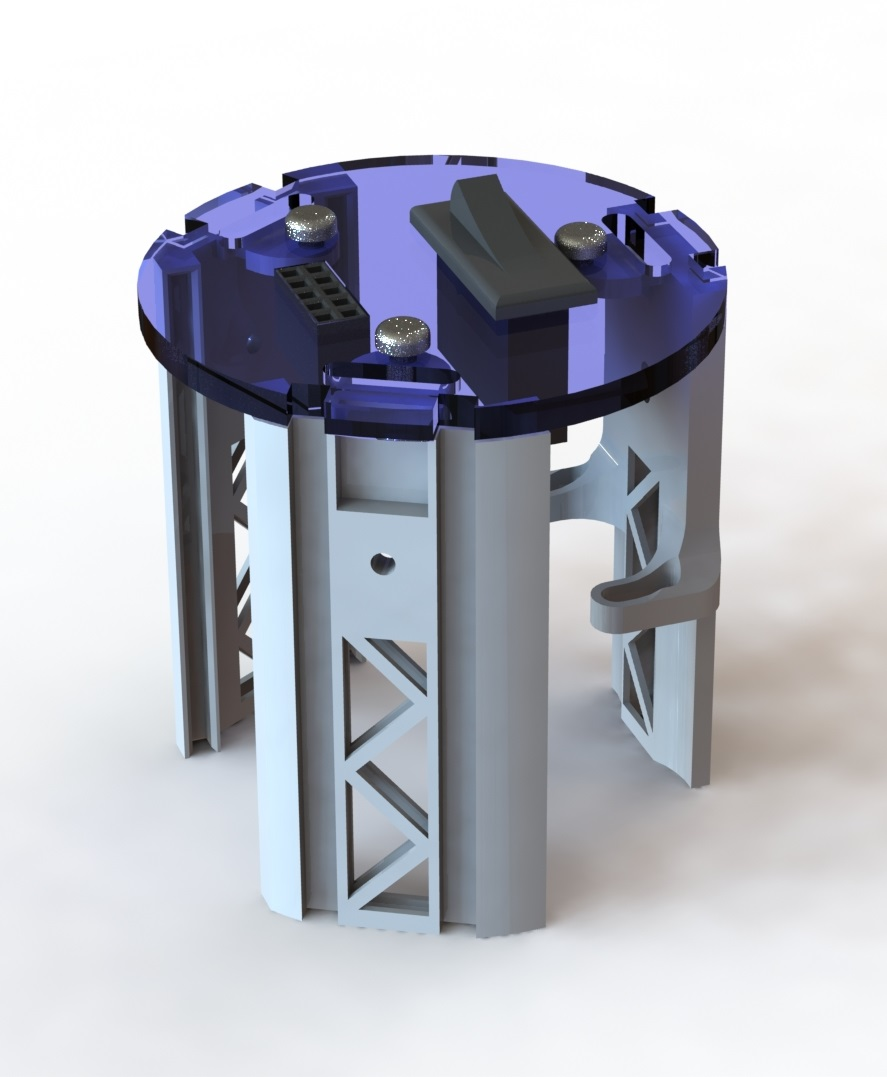
\includegraphics[scale=0.4]{Top_frame_render.jpg}\hspace*{\fill}
			\caption{Final CanSat top frame render}
			\label{topframerender}
		\end{figure}
		
		The bottom frame was more complex. The basic frame was designed as a single piece of material, again with outer shell, PCB, and battery mount and hold points. Additionally, the bottom frame includes a mounting plate for an Omron D6T thermal camera, as well as screw holes to allow for add-on modules to be attached to the CanSat. Currently, these screw holes are occupied by a piece of laser-cut plastic providing a protective bezel for the thermal camera, seen in figure \ref{bottomframerender}.
		
		%\begin{wrapfigure}{L}{0.5\textwidth}
		%	\begin{center}
		%		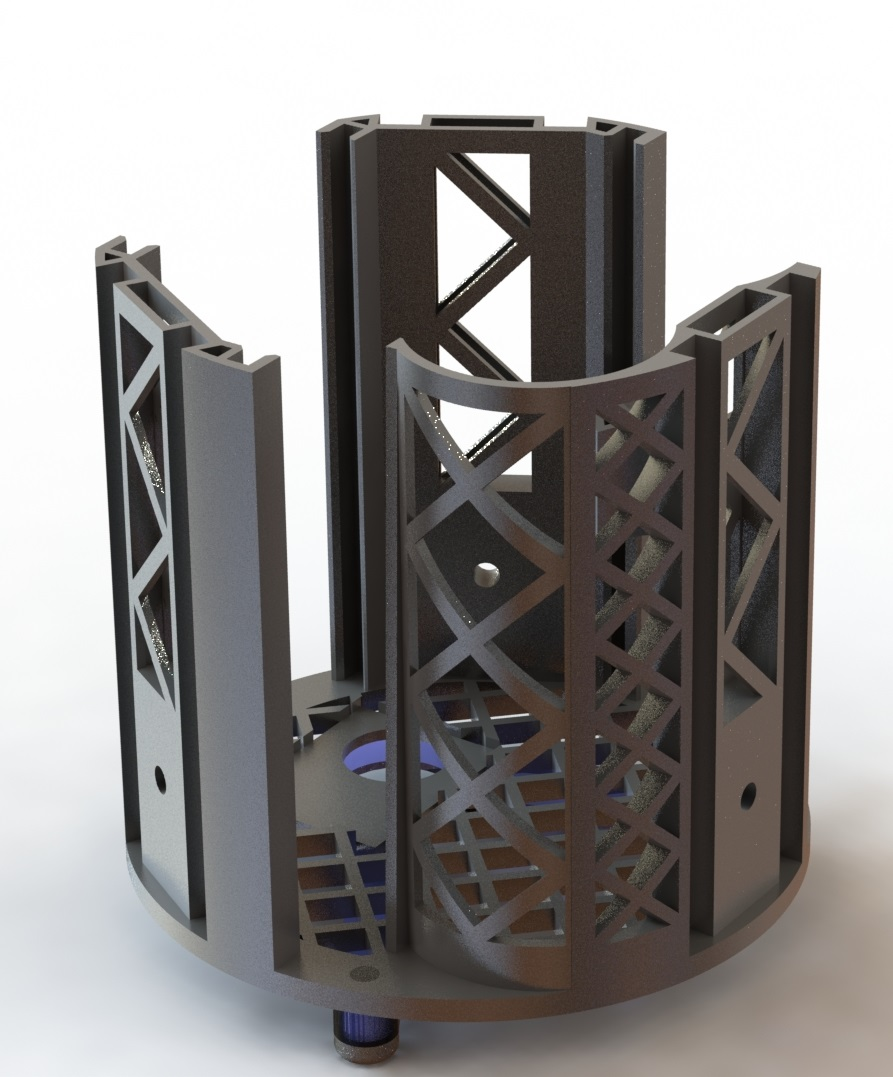
\includegraphics[scale=0.4]{Bottom_frame_render.jpg}
		%	\end{center}
		%	\caption{Final CanSat bottom frame render}
		%	\label{bottomframerender}
		%\end{wrapfigure}
		
		\begin{figure}[h]
			\hfill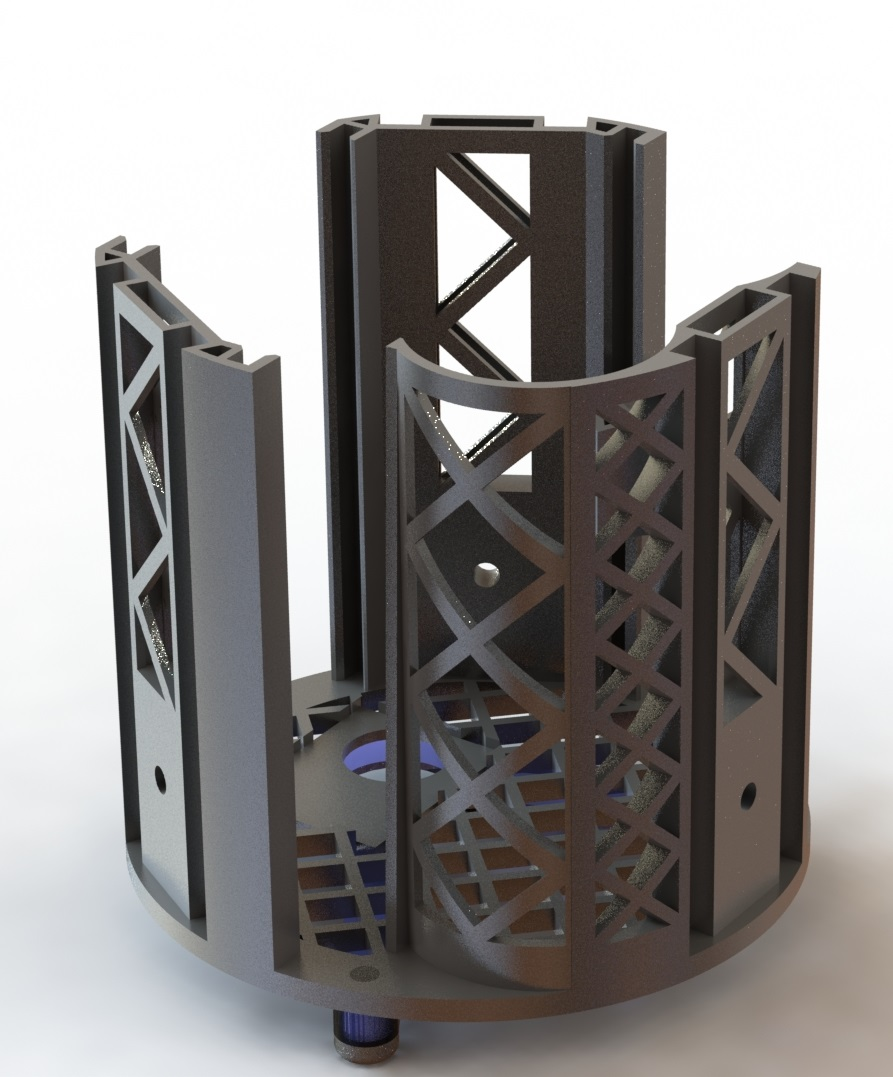
\includegraphics[scale=0.4]{Bottom_frame_render.jpg}\hspace*{\fill}
			\caption{Final CanSat bottom frame render}
			\label{bottomframerender}
		\end{figure}
		
		The internal frame was initially designed to be printed from PLA in a consumer 3D printer. However, we found that this did not provide the desired tolerances. This is clearly seen in the image in figure \ref{plaframe}.
		
		\begin{figure}[h]
			\hfill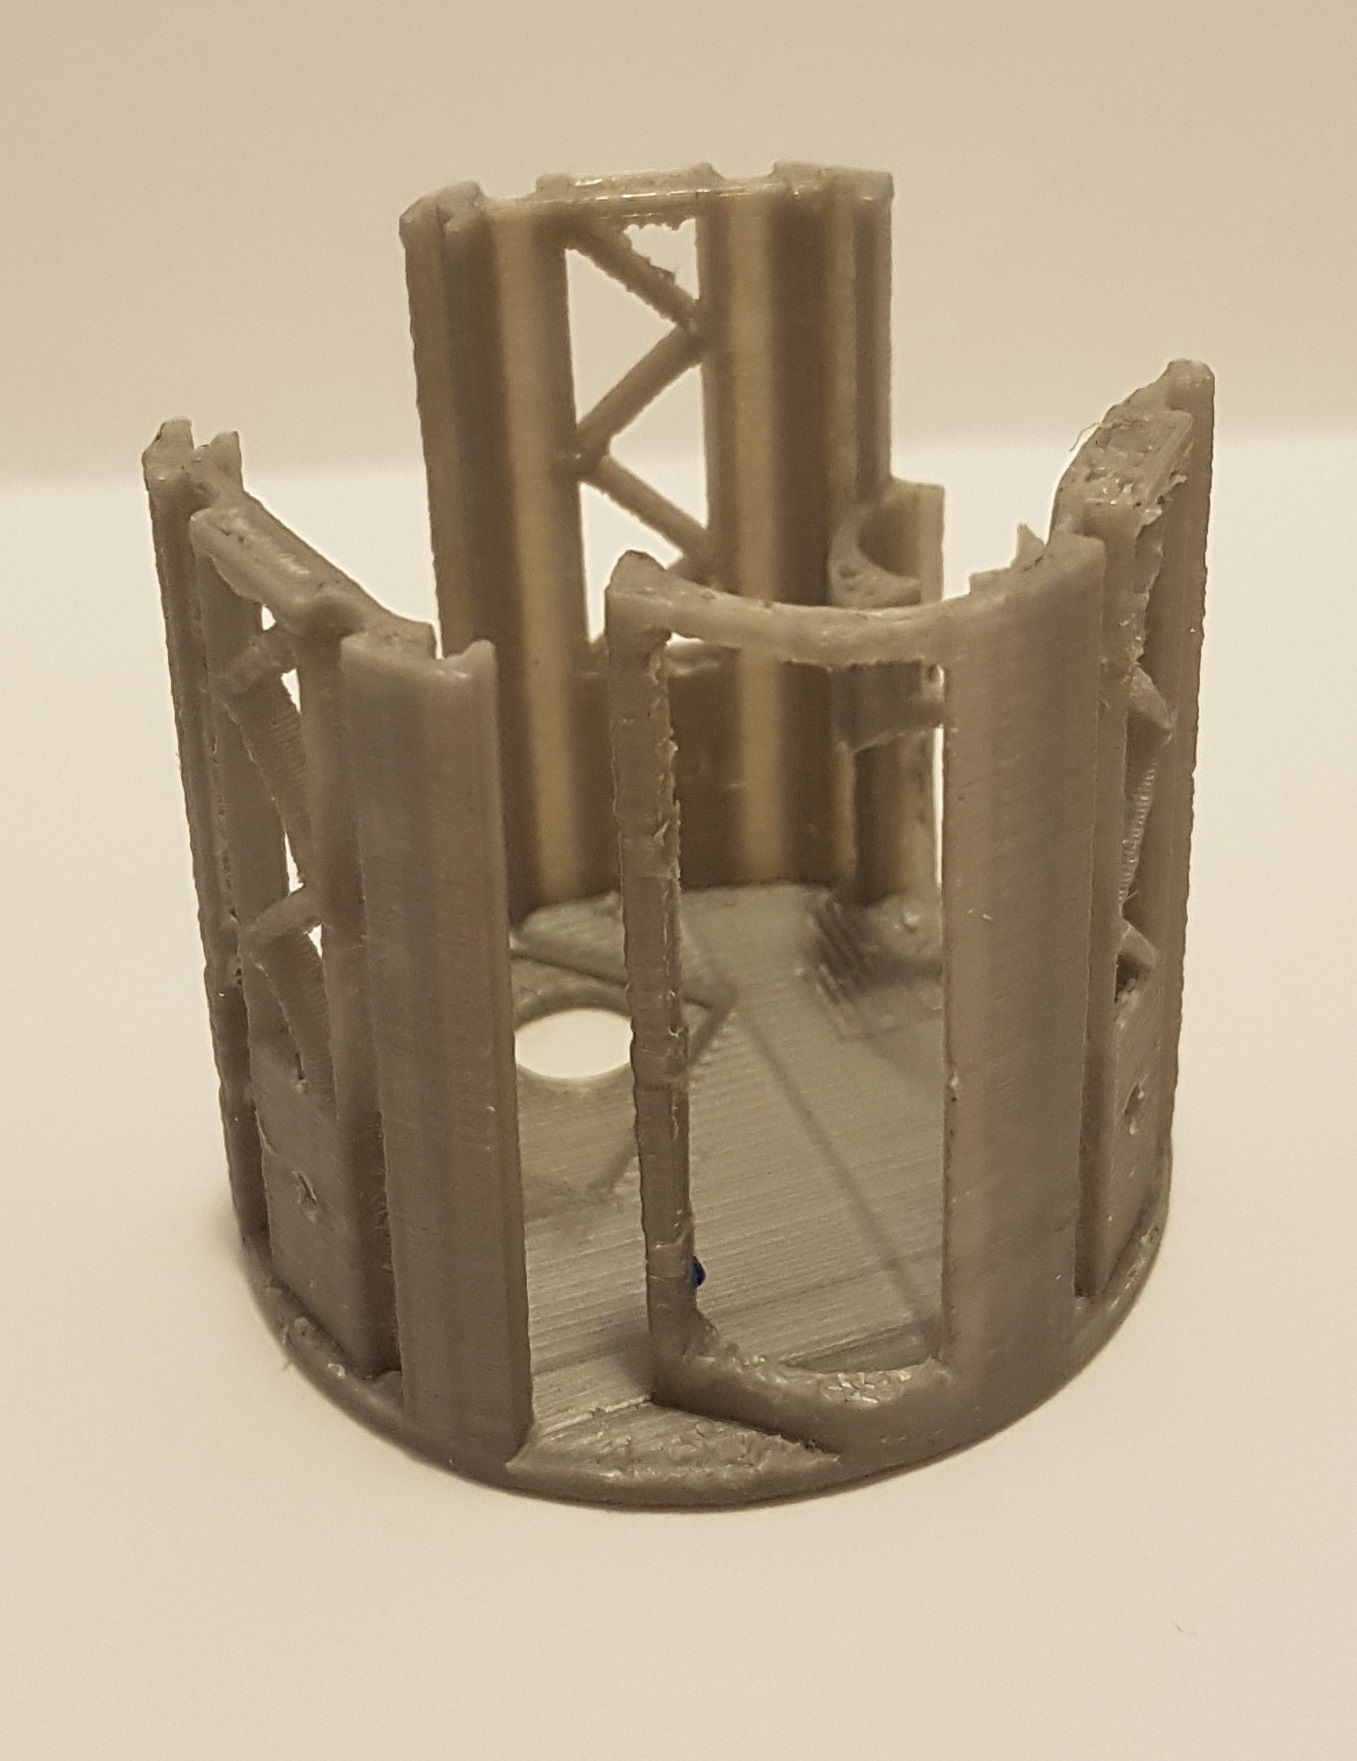
\includegraphics[scale=0.15]{pla_frame.jpg}\hspace*{\fill}
			\caption{A 3D printed PLA CanSat bottom frame}
			\label{plaframe}
		\end{figure}
		
		
		Croft additive manufacturing offered to sponsor the team with an SLS (selective laser sintering) internal frame built from stainless steel, seen in figure \ref{steelframe}.
		
		\begin{figure}[h]
			\hfill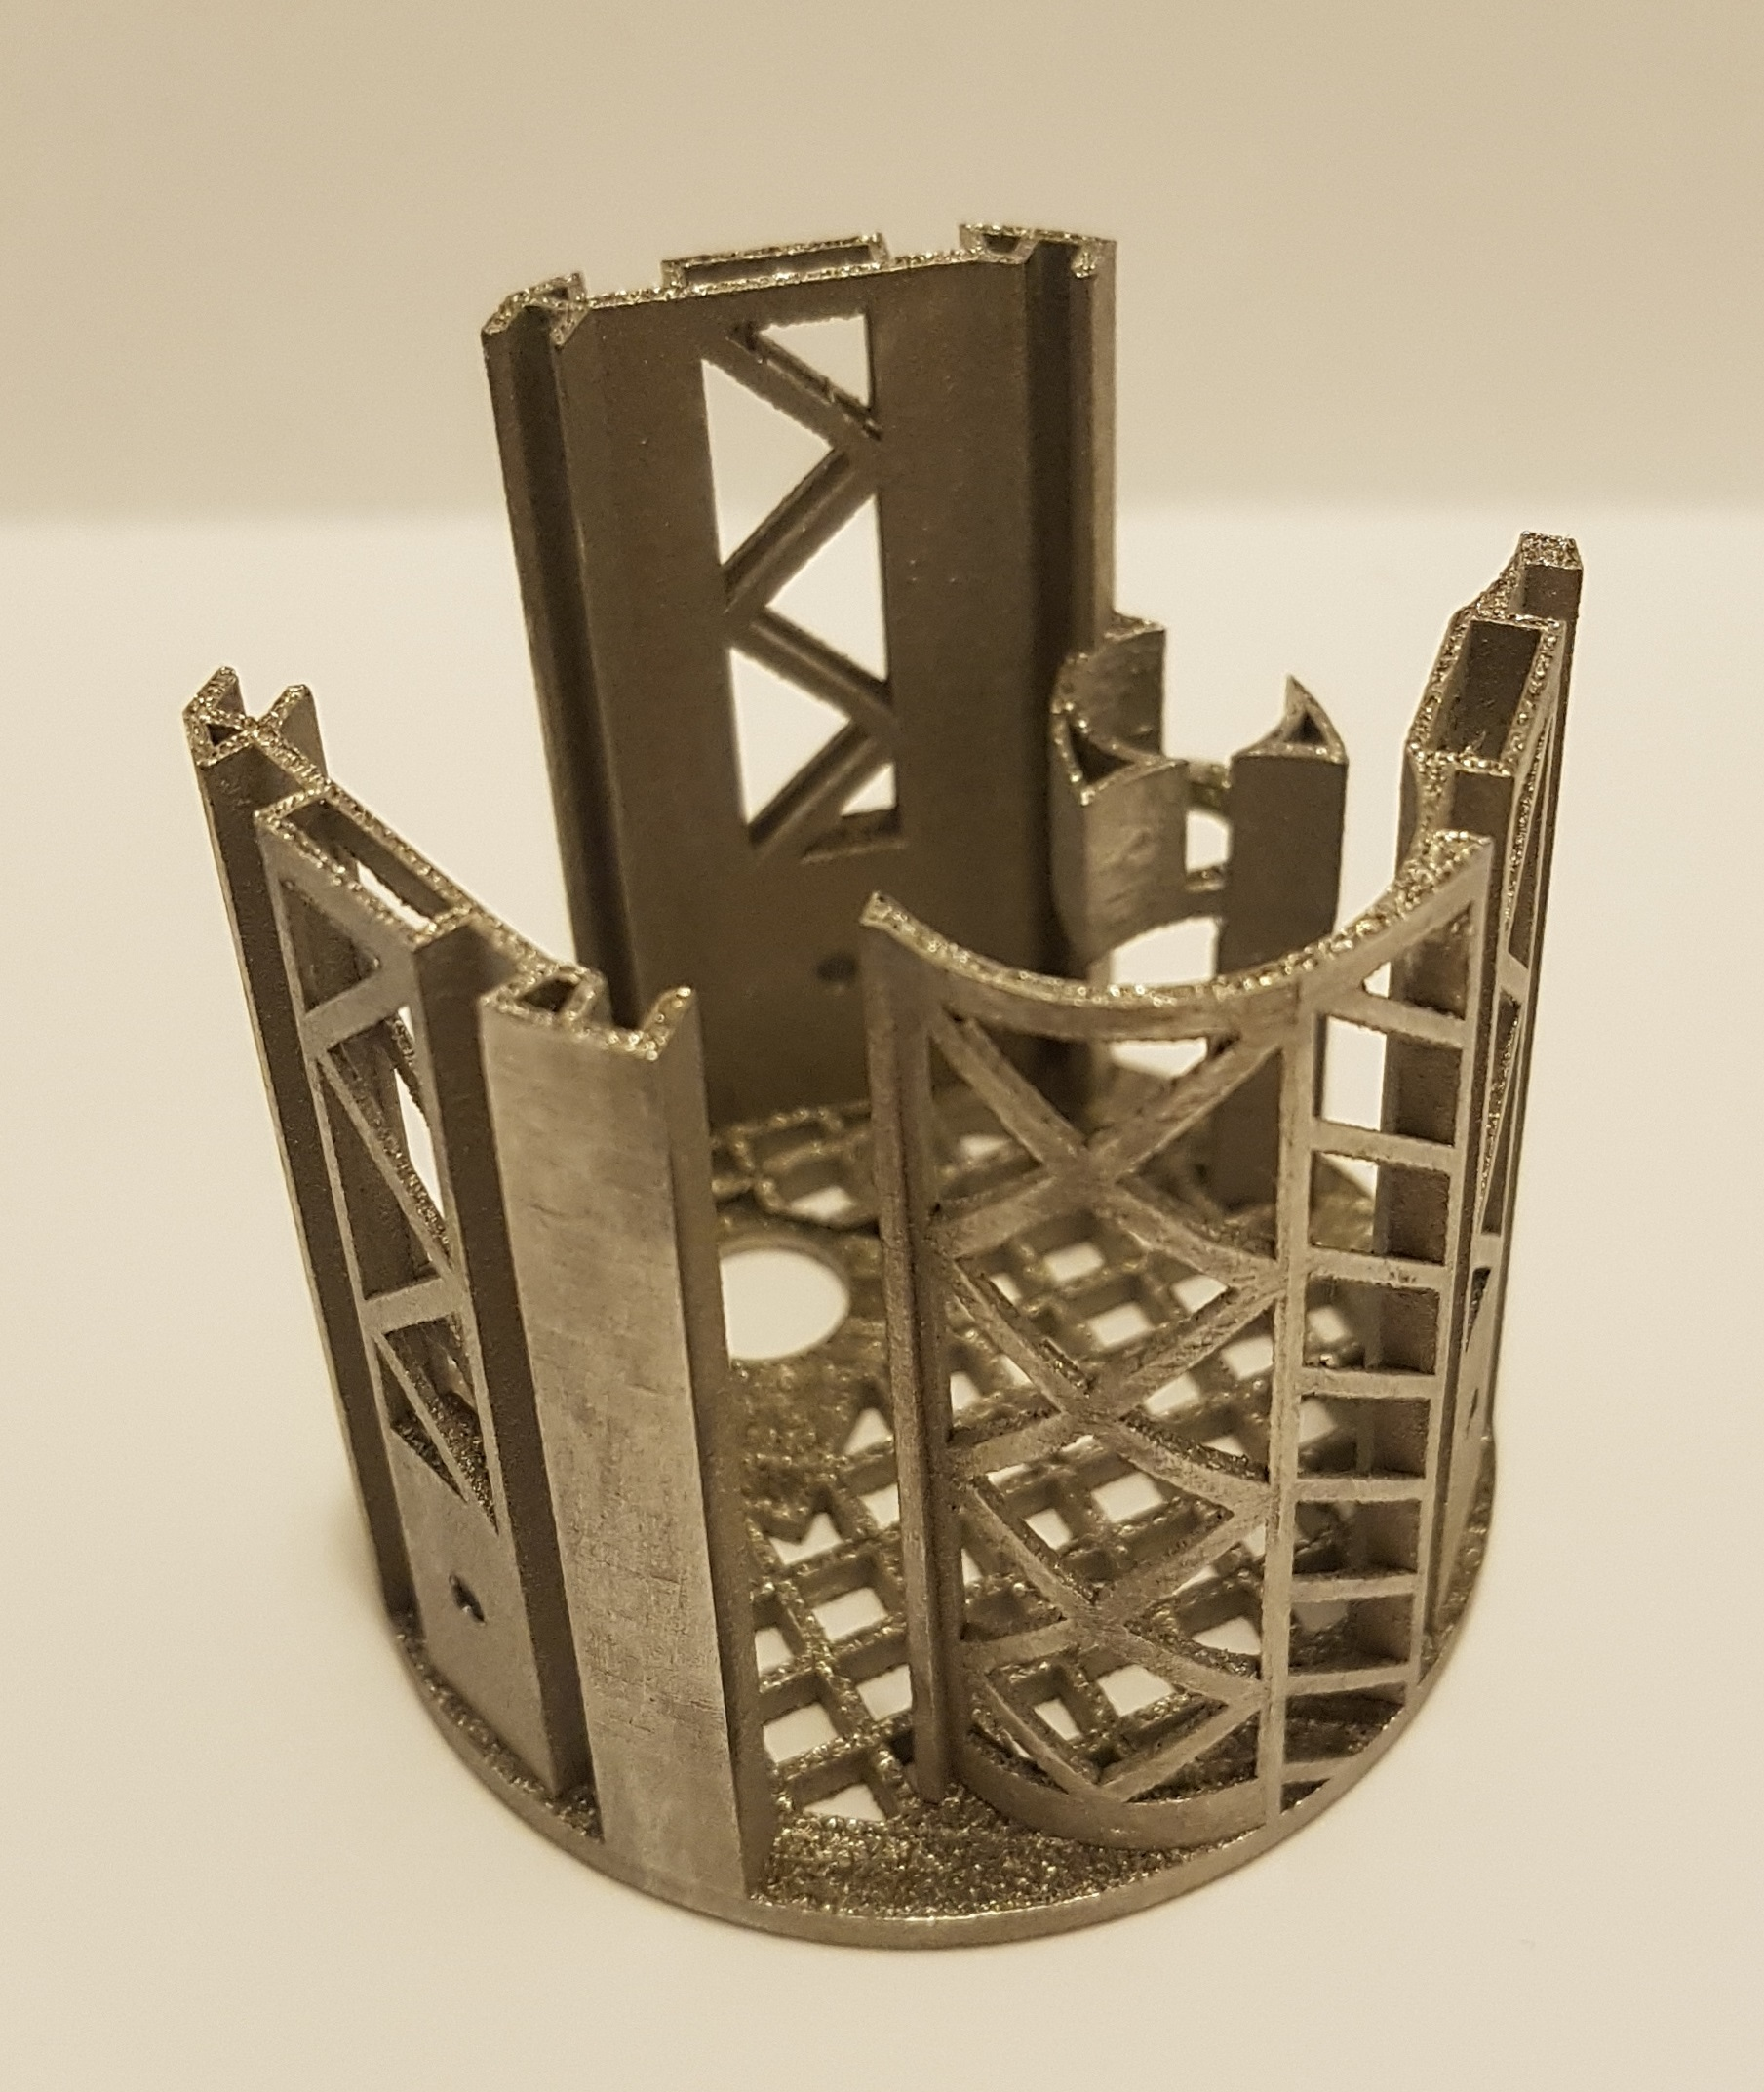
\includegraphics[scale=0.15]{steel_frame.jpg}\hspace*{\fill}
			\caption{A 3D printed steel CanSat bottom frame}
			\label{steelframe}
		\end{figure}
		
		This construction did allow for required tolerances but lead to near-maximum mass for the entire CanSat, preventing the team from pursuing any further add-on modules. A conductive steel frame also led to radio range reduction in our testing.
		
		The team then ordered a nylon frame to be constructed via Shapeways again via SLS- this is shown in figure \ref{nylonframe}.
		
		\begin{figure}[h]
			\hfill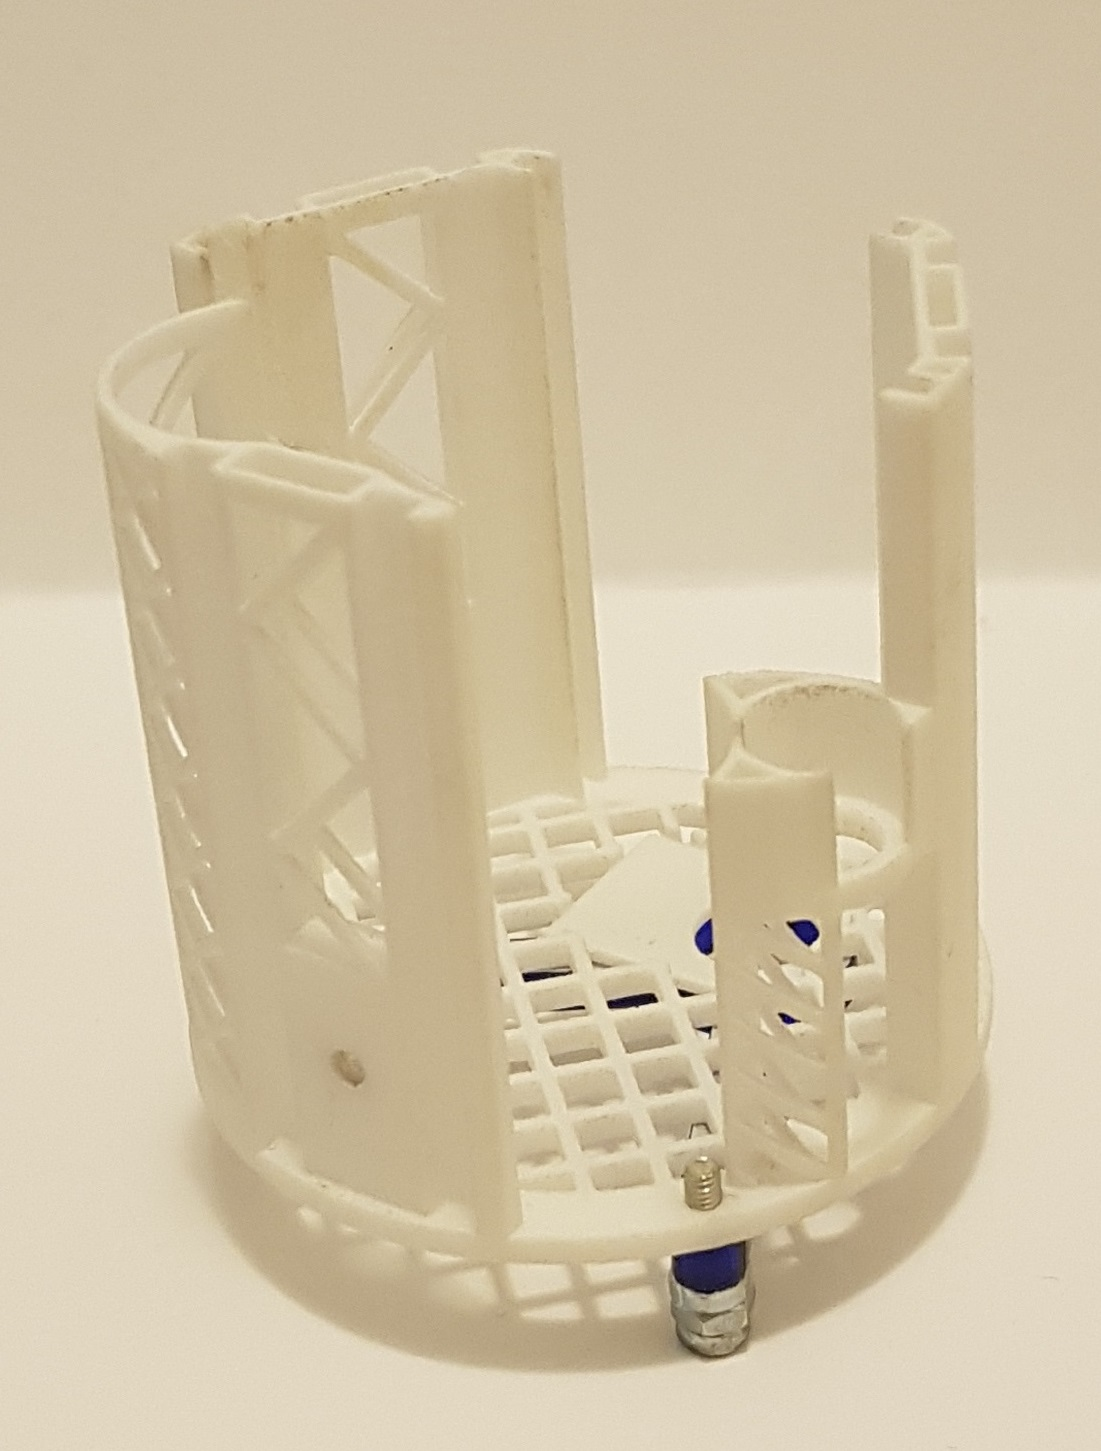
\includegraphics[scale=0.15]{nylon_frame.jpg}\hspace*{\fill}
			\caption{A 3D printed nylon CanSat bottom frame}
			\label{nylonframe}
		\end{figure}
		
		A nylon internal frame, while more flexible than desired, allowed for minimal weight while retaining the toughness and tolerances that our design required while remaining suitably affordable. In order to minimize the flexibility of the internal frame, the team has decided to use a steel top frame paired with a nylon bottom frame.
		
		\subsubsection{Outer Shell}
		
		The team again elected to use a fiberglass outer shell. In order to improve tolerances, a mold was 3D printed out of PLA and covered with aluminum foil before the casting process began- the mold and a shell are visible in figure \ref{shellmold}.
		
		\begin{figure}
			\centering
			\begin{subfigure}{.5\textwidth}
				\centering
				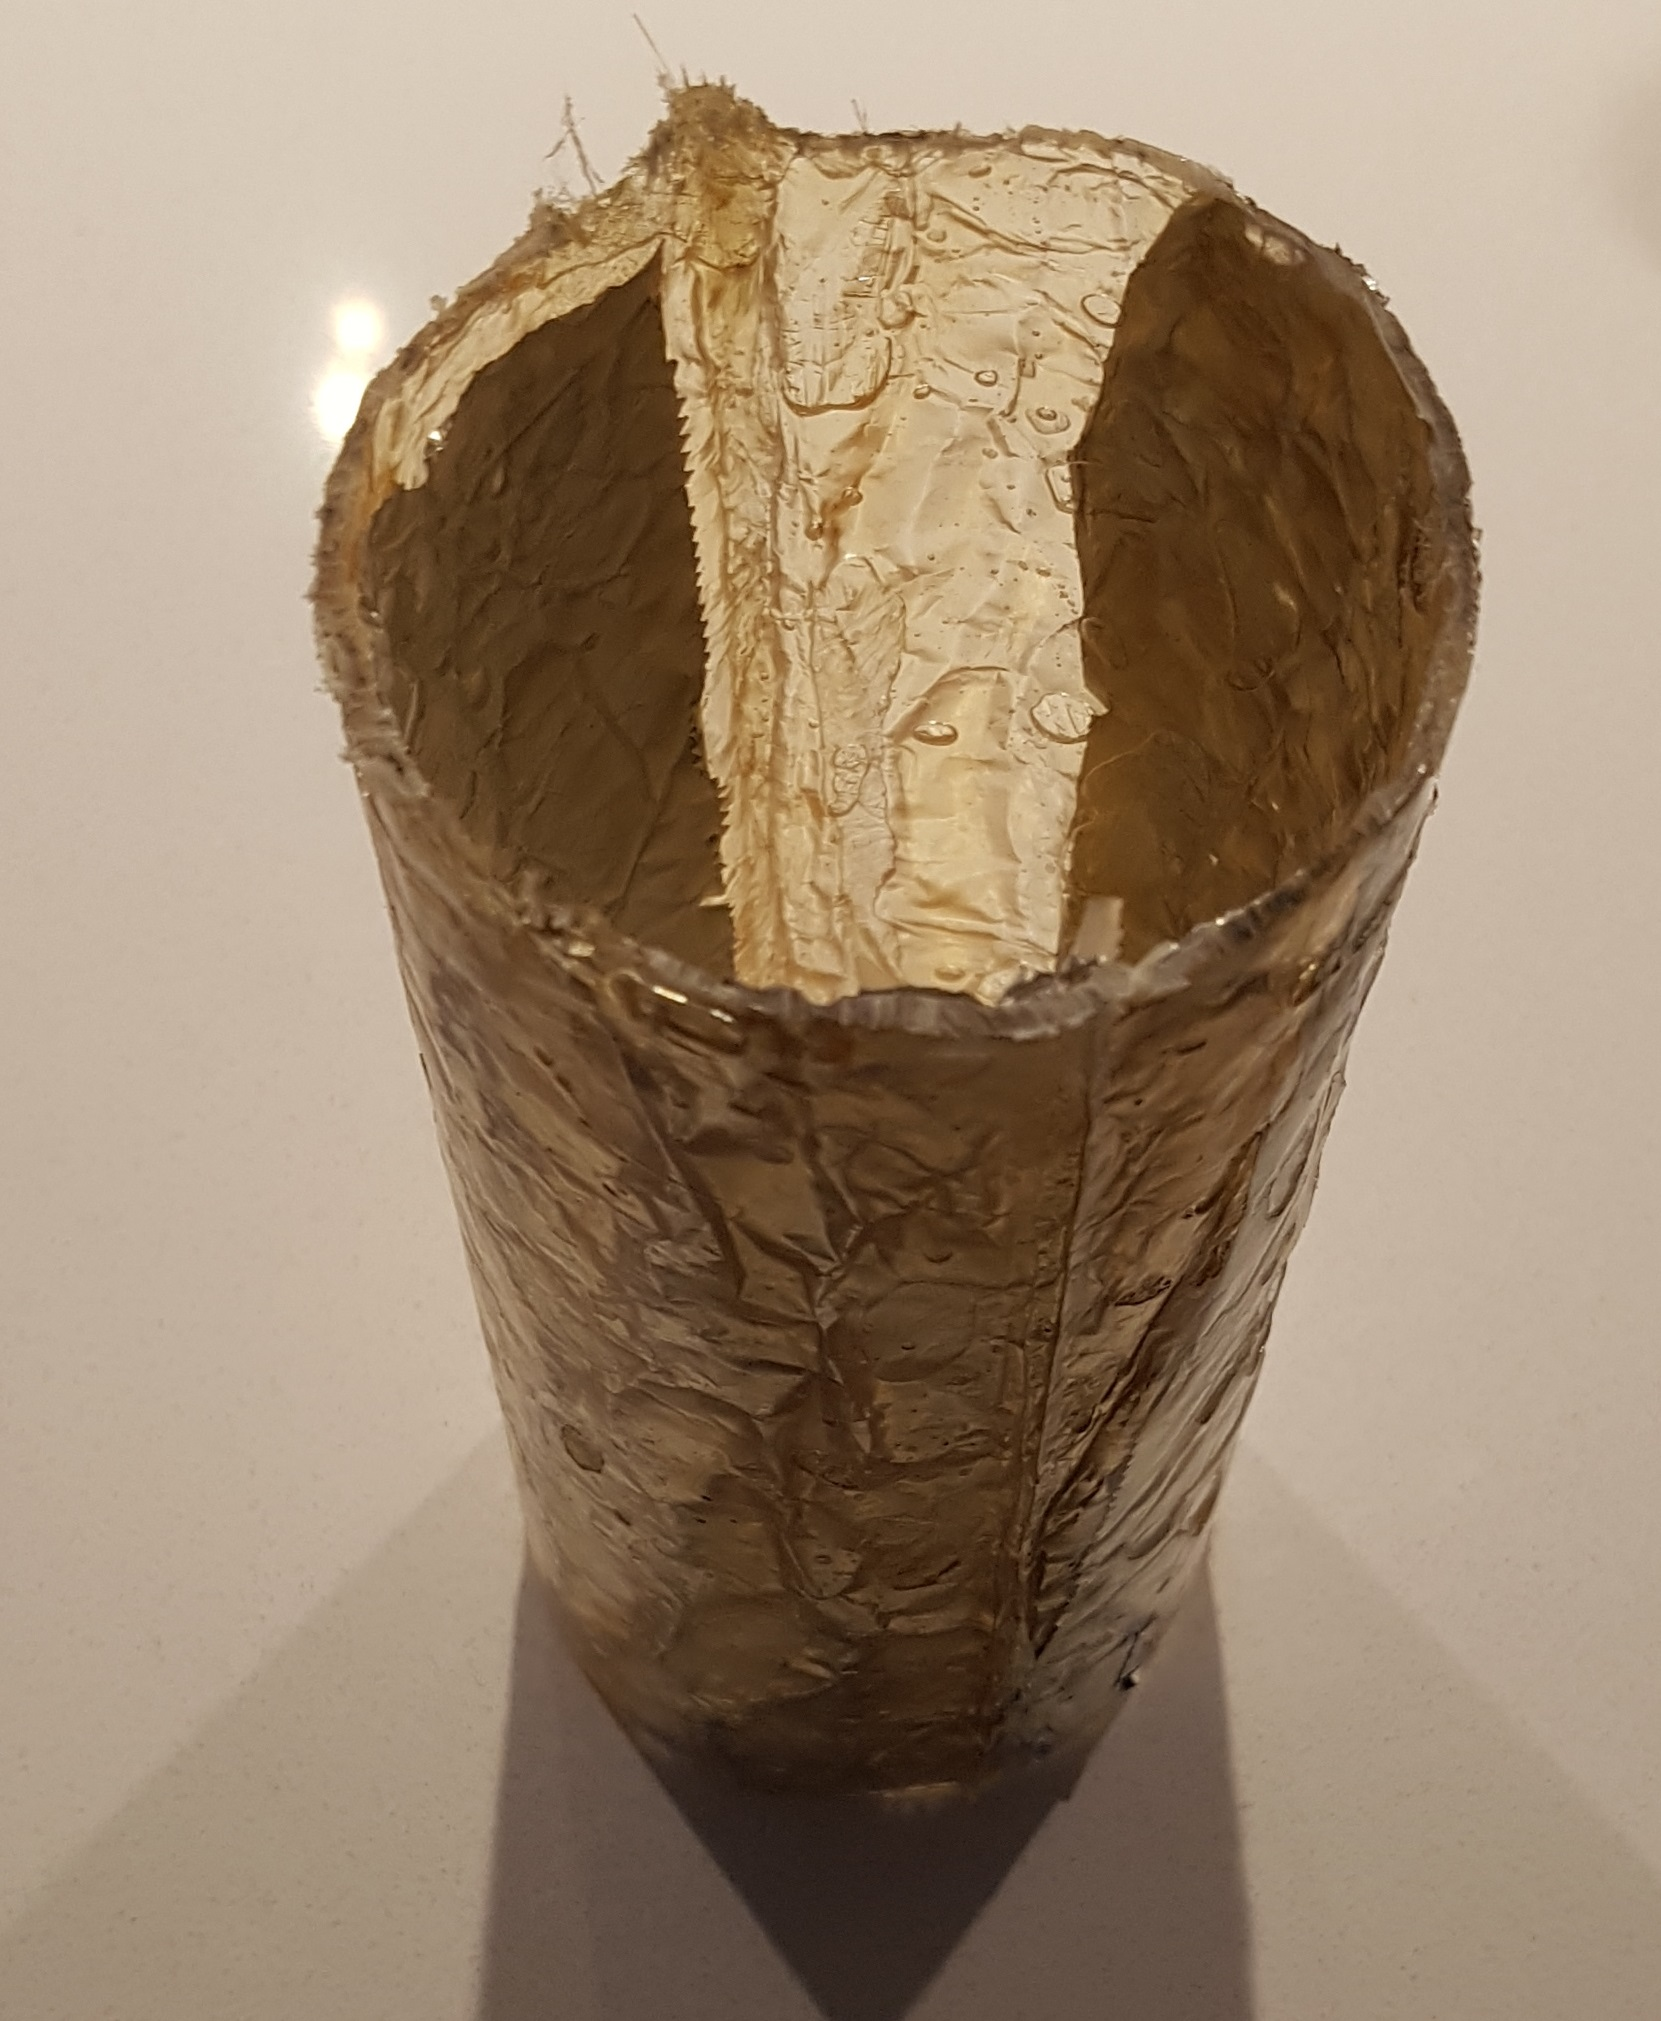
\includegraphics[width=.8\linewidth]{rawshell.jpg}
			\end{subfigure}%
			\begin{subfigure}{.5\textwidth}
				\centering
				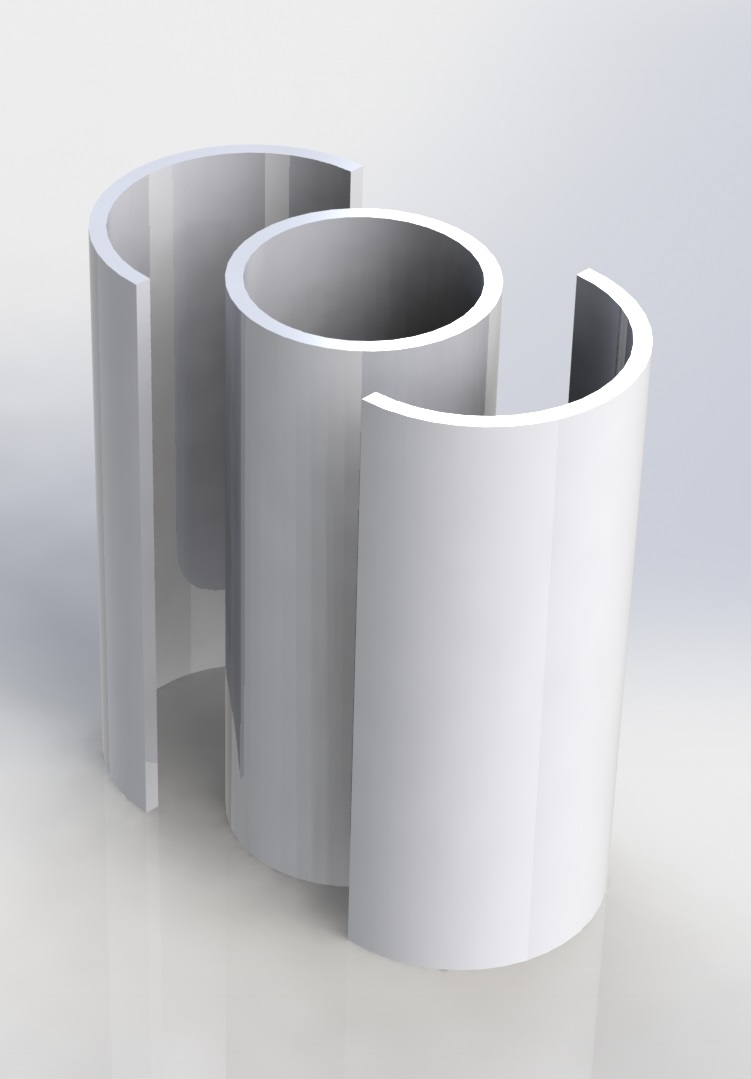
\includegraphics[width=0.7\linewidth, angle=0]{Mold_render.jpg}
			\end{subfigure}
			\caption{A raw outer shell with a render of its mold}
			\label{shellmold}
		\end{figure}
		
		In order to minimize the mounting difficulties found in the CanSat prototype, the team decided on a slider system built from 3D printed PLA to allow for outer shell – internal frame mounting, secured via a set of bolts. This mechanism is visible in figure \ref{sliders}. While this system would lack the shock resistance of the CanSat prototype the team believed it to be a worthwhile tradeoff. 
		
		\begin{figure}
			\centering
			\begin{subfigure}{.5\textwidth}
				\centering
				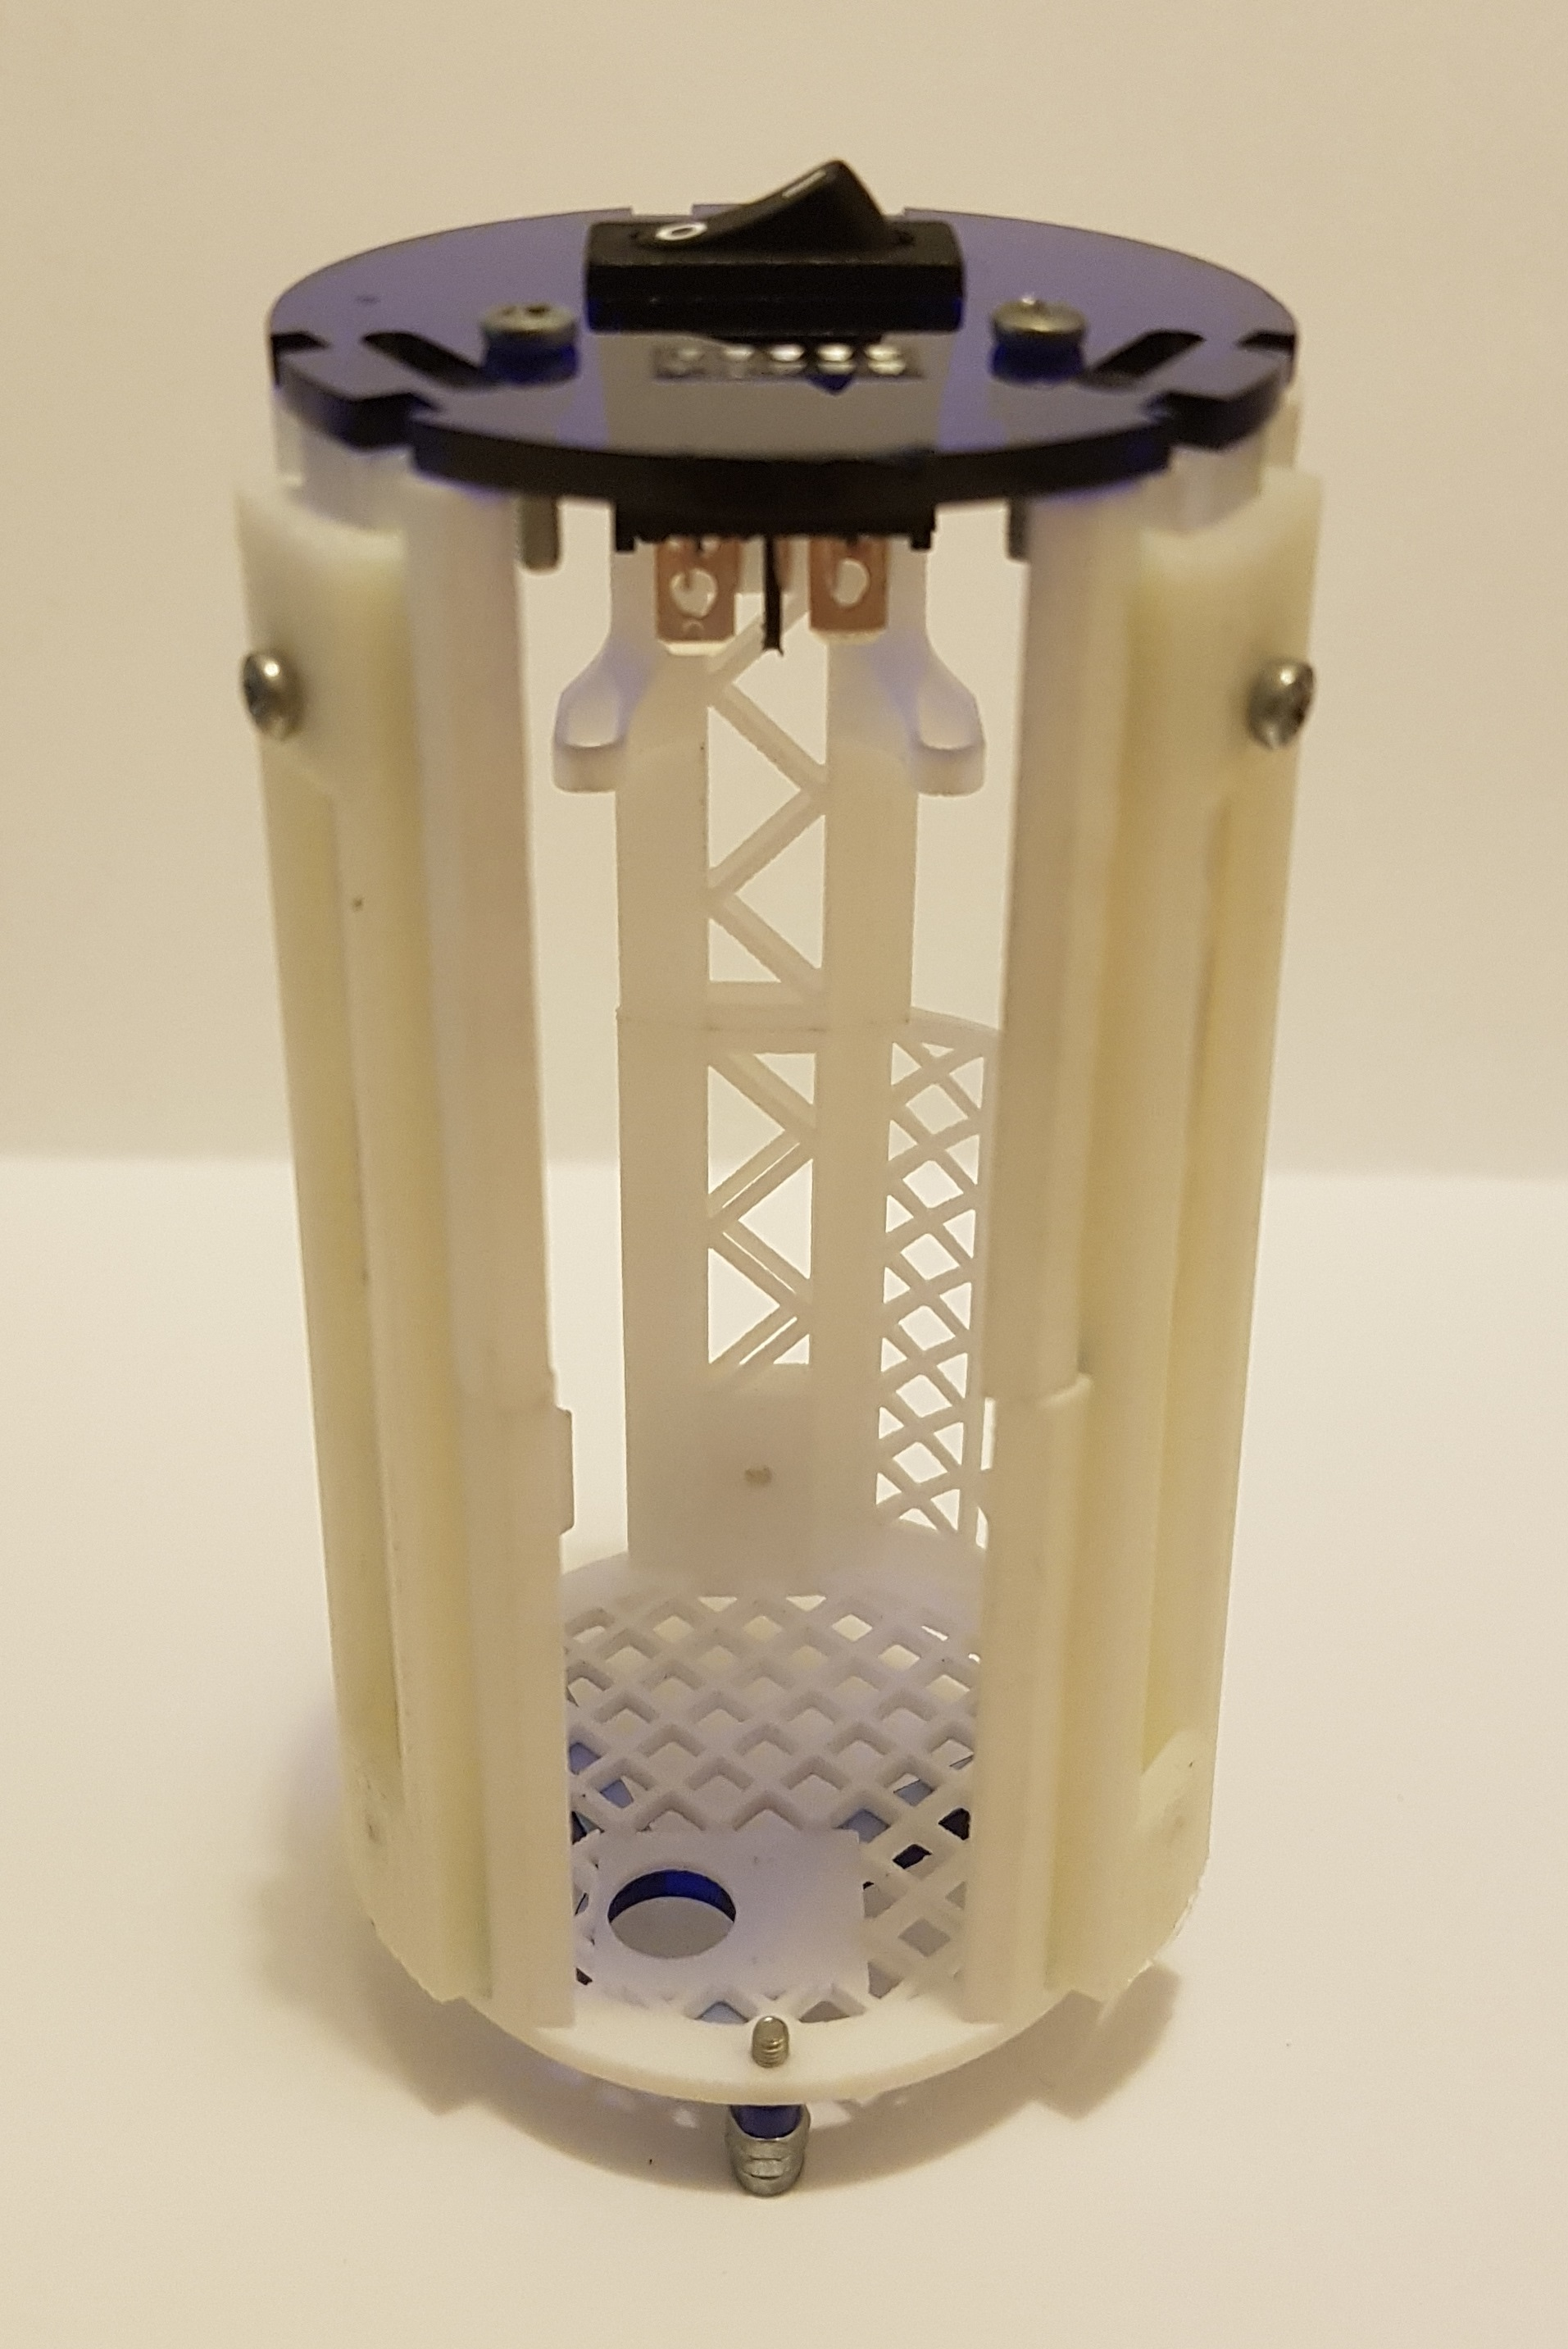
\includegraphics[width=.7\linewidth]{bareframe.jpg}
			\end{subfigure}%
			\begin{subfigure}{.5\textwidth}
				\centering
				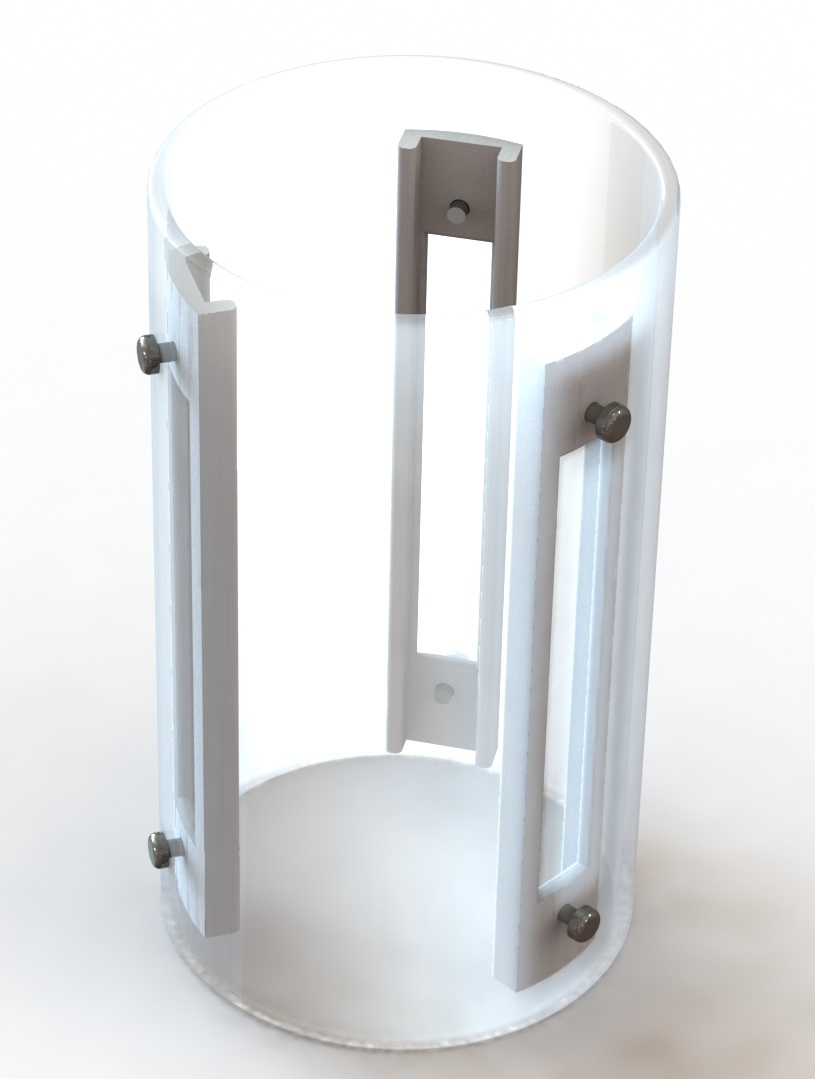
\includegraphics[width=0.8\linewidth, angle=0]{Outer_shell_render.jpg}
			\end{subfigure}
			\caption{The CanSat slider mechanism}
			\label{sliders}
		\end{figure}
		
		
		\subsubsection{Electronics Mounting}
		
		The team maintained a similar sensor payload in the second CanSat revision, although the use of new sensors allowed us to condense the pressure and humidity sensors into one unit. A more advanced internal frame design also allowed for easier and more secure battery and electronics mounting, illustrated in figure \ref{elecmount}.
		
		\begin{figure}[h]
			\hfill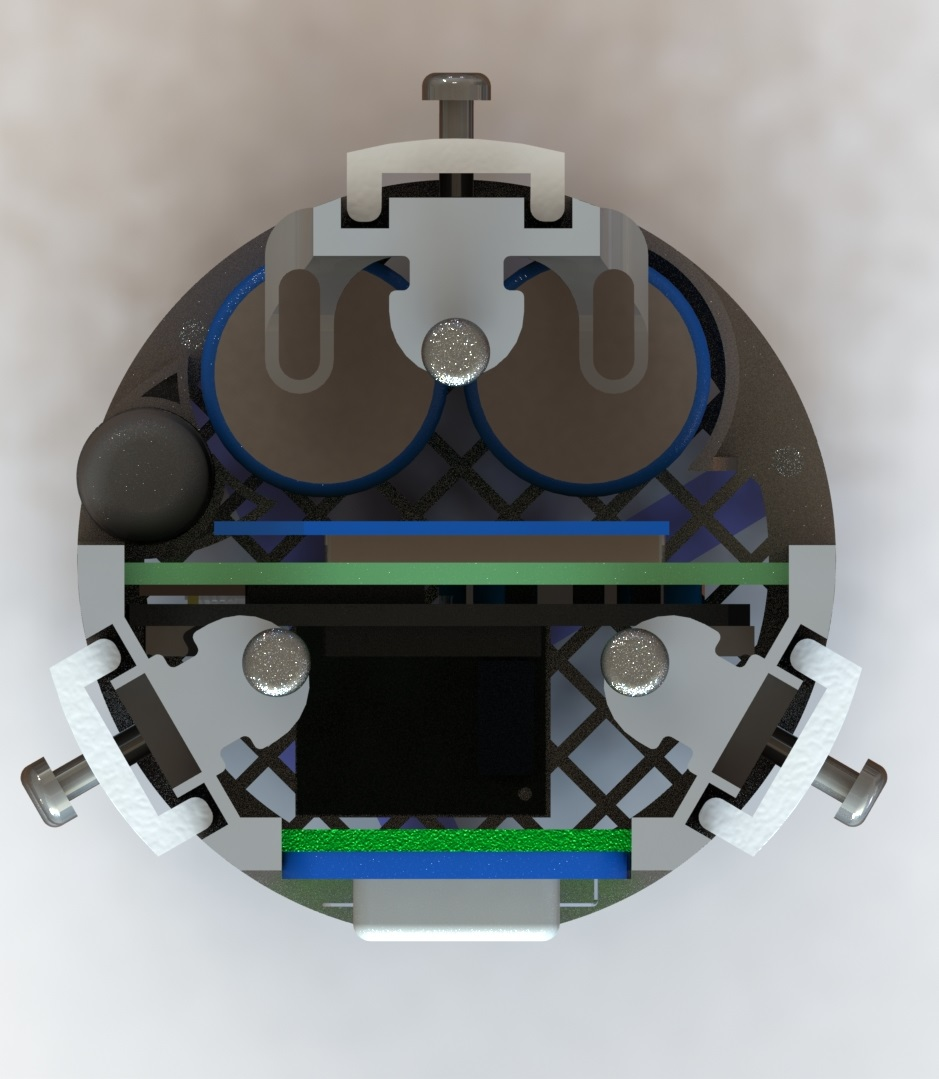
\includegraphics[scale=0.5]{electronics_mount_render.jpg}\hspace*{\fill}
			\caption{A render illustrating electronics mounting in the final CanSat}
			\label{elecmount}
		\end{figure}
		
		
	\subsection{Electrical Design}
		
		\subsubsection{Sensor and Device Wiring}
		
		As mentioned earlier, the electrical design remained relatively constant between revisions. The largest electrical change was in deciding to design custom PCBs to maximize available sensor mounting space, visible in figure \ref{pboardnew}. 
		
		With custom PCBs, we were able to include surface mount components. This allowed us to mount supporting GPS, XBEE, and level shifting circuitry directly on the PCB, removing the need for expensive breakout boards. We also decided to use the CHIP Pro instead of the CHIP: while it only included 512MB of Flash and 256MB of RAM, it promised lower power consumption and a PCB friendly footprint. We also used a BME280, replacing the DHT22 and BMP180, and offering humidity, pressure, and temperature sensors.
		
		Fearing radio range concerns the team moved from 2.4GHz XBEE-Pro modules to 868MHz XBEE-LP radios, which offer a range of 5km at 10Kbps. The 868MHz XBEE radios are also surface-mount-compatible, reducing space requirements further.
		
		\begin{figure}[h]
			\hfill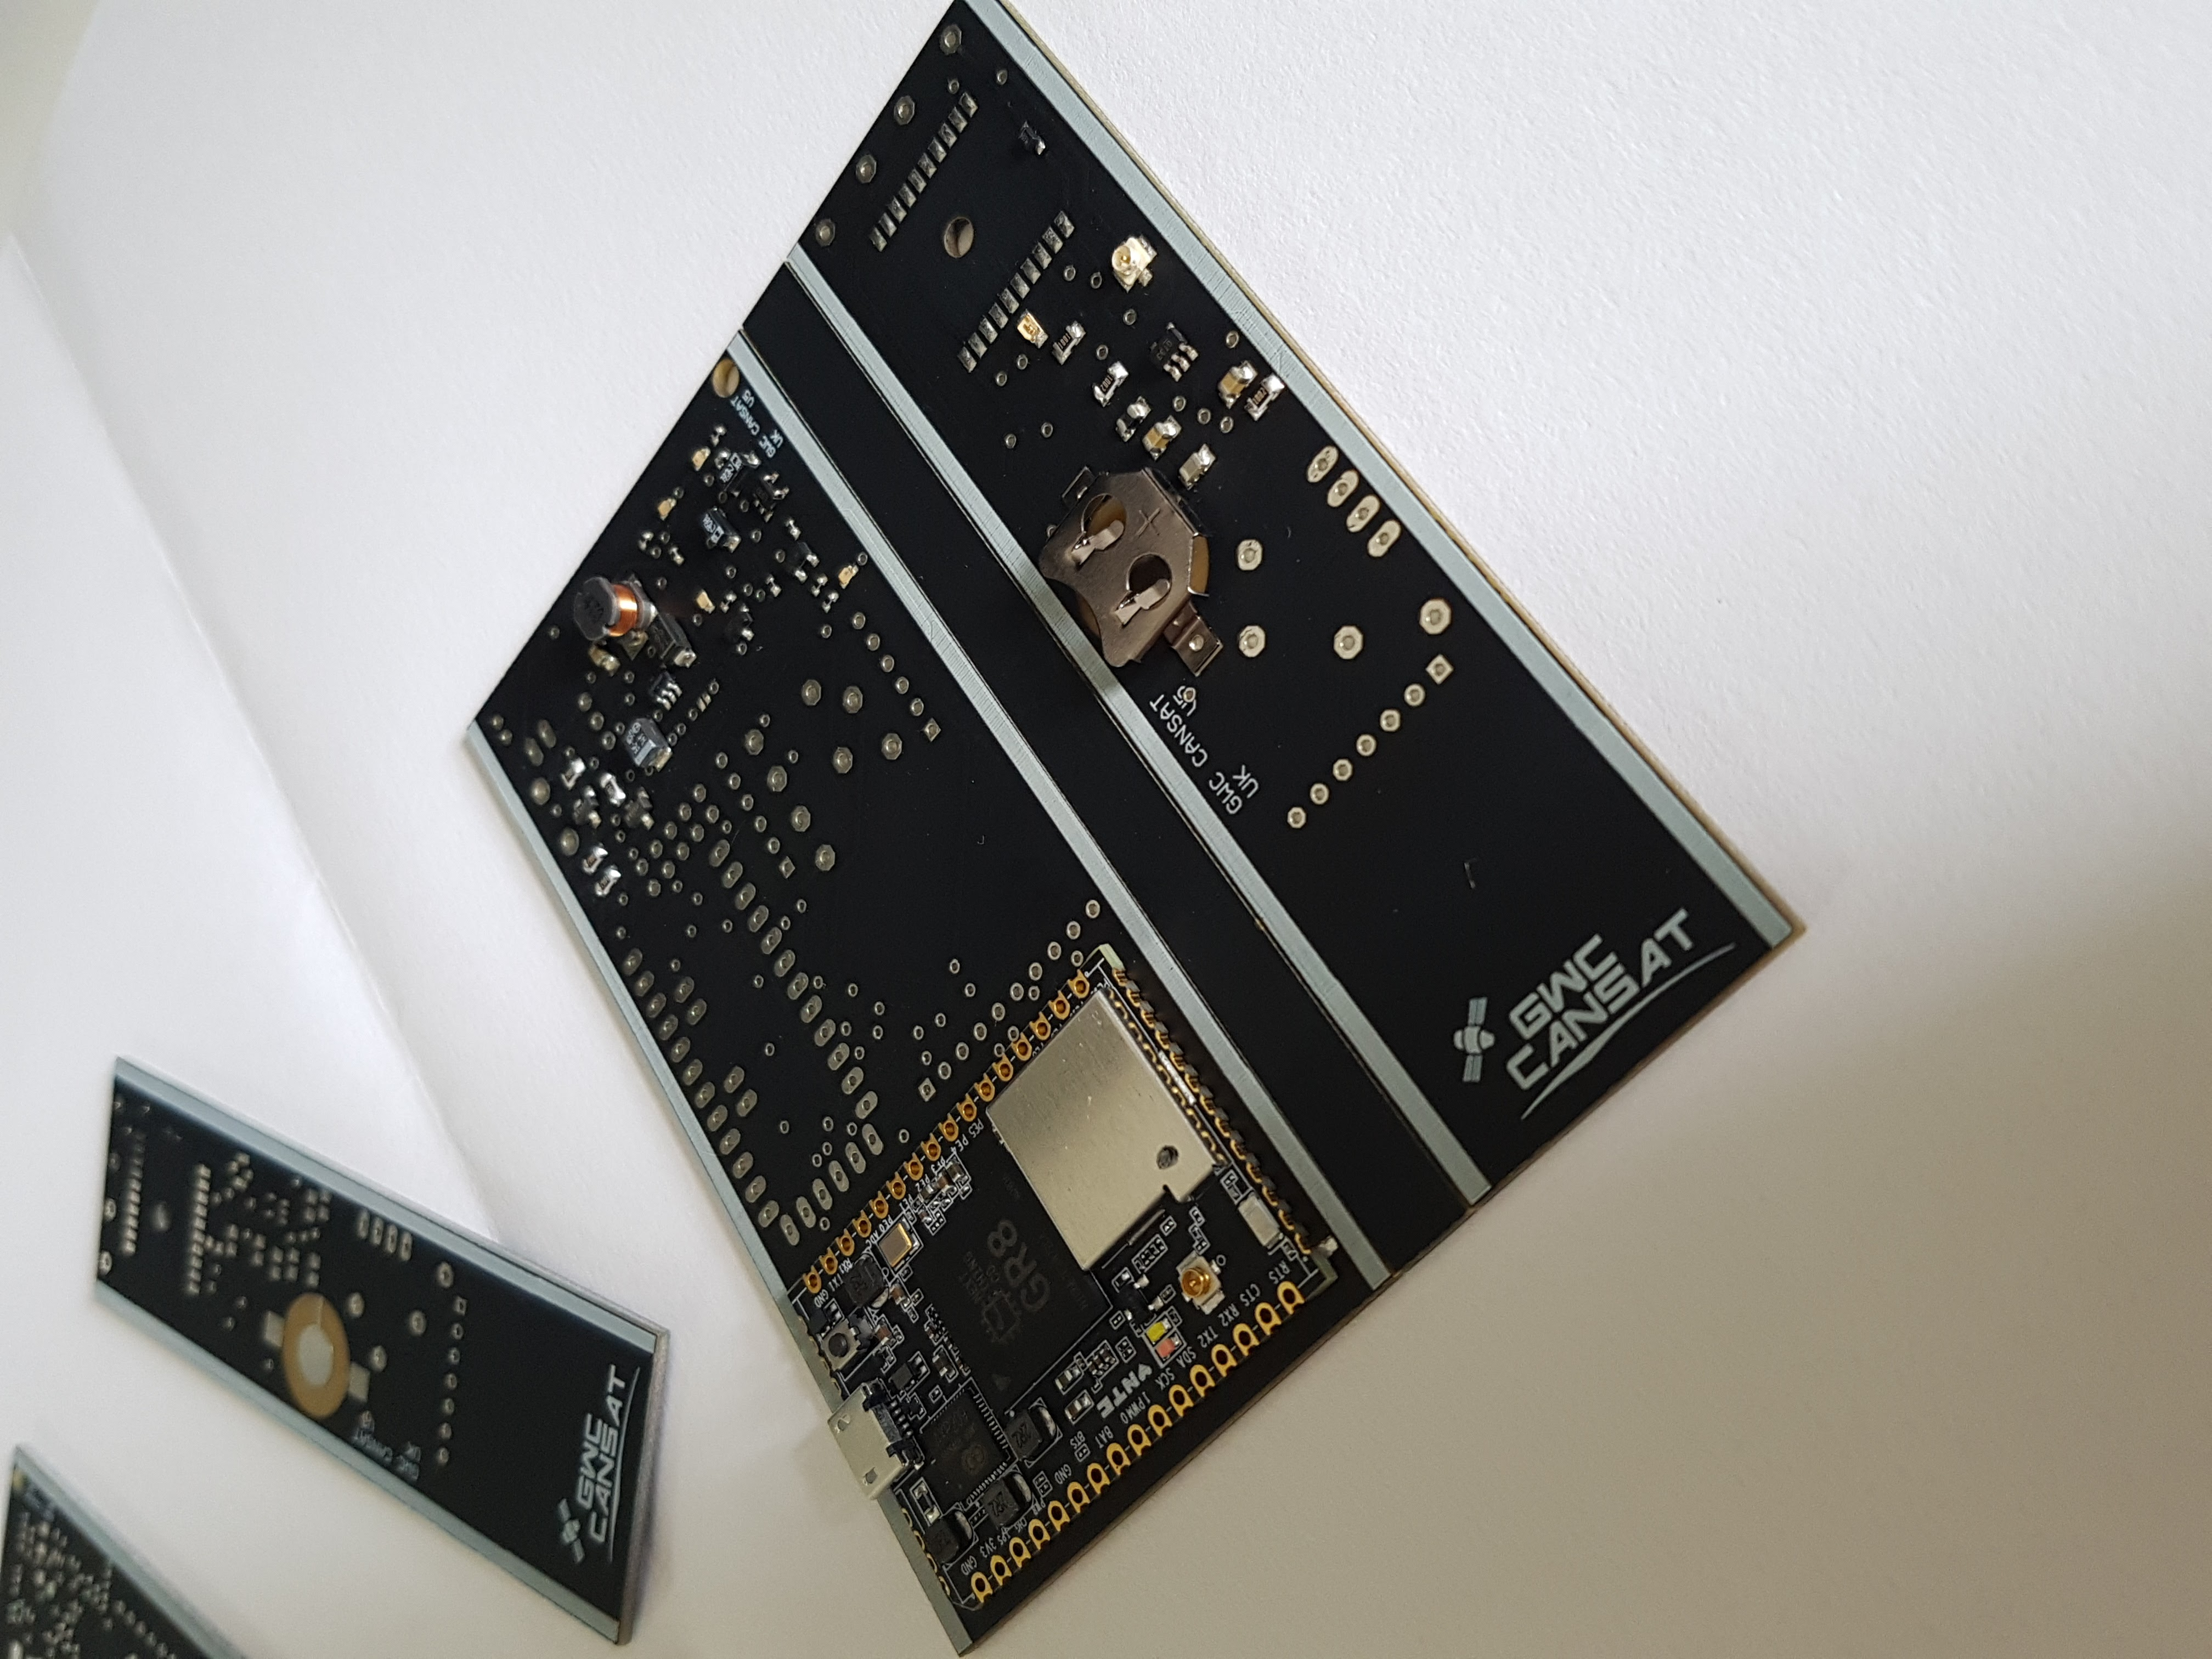
\includegraphics[scale=0.1, angle=270]{pcbs.jpg}\hspace*{\fill}
			\caption{Partially assembled CanSat PCBs}
			\label{pboardnew}
		\end{figure}
		
		With our new internal frame design the team was able to expand to two PCBs: a primary PCB with control, radio, and some sensor circuitry, and a secondary PCB with a larger array of sensors. We also included redundant level shifting and step-down voltage converters to ensure a reliable system.
		
		As with our mechanical design, the team's electrical schematics and layouts are available at the team GitHub \footnote{https://github.com/Arcturus314/cansat2017\_design}, though a condensed schematic is shown in figure \ref{cschem}.
		
		\begin{figure}[h]
			\hfill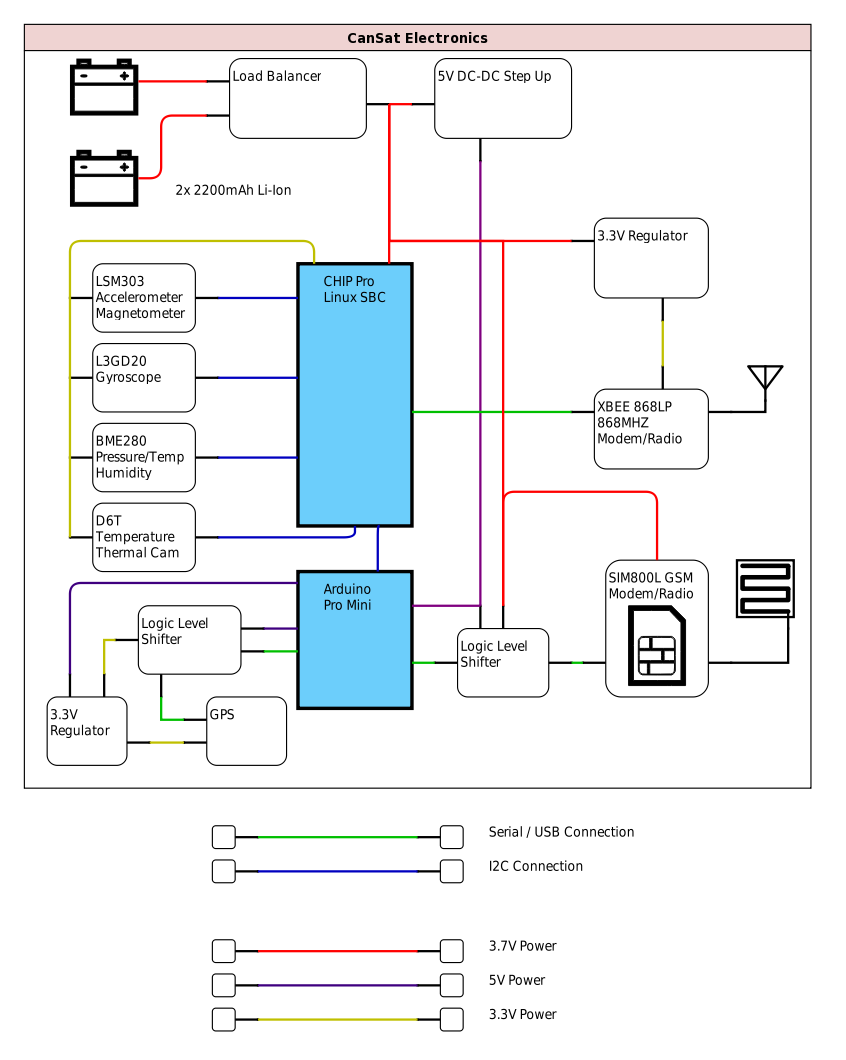
\includegraphics[scale=0.7]{CanSat-detail.png}\hspace*{\fill}
			\caption{A condensed schematic of the final CanSat}
			\label{cschem}
		\end{figure}
		
		\subsubsection{Radio Specifications}
			
		The team decided to continue using the SIM800L in the final CanSat design due to its ease of use. However, the move to custom PCBs allowed the team to utilize the XBEE 868LP \footnote{https://www.digi.com/products/xbee-rf-solutions/sub-1-ghz-modules/xbee-868lp}: the only other long range XBEE module permitted for use in the European Union, which operates as a spread-spectrum device at 863-870MHz. The XBEE 868LP has the added benefits of lower power consumption at 48mA and a longer maximum range of 8.4km. These characteristics lead to a smaller transmit rate of 10kbps. However, the team accepted this loss due to the smaller packets resulting from rewritten CanSat code.
		
		\subsubsection{Battery Specifications and Estimated Runtime}
		
		As mentioned earlier, battery choice has remained constant between our prototype and final CanSats, and hence will not be restated here.
		
		\subsection{Software Design}		
		
		\subsubsection{On-CanSat}
		The CanSat software is divided between the main control, data logging, and processing loops running on the Linux SBC, and the control and interpretation loop running on the Arduino Pro Mini. All of our CanSat code is available in our team's software GitHub repository \footnote{https://github.com/Arcturus314/cansat2017}.
		\subsubsection{Linux Single-Board-Computer}
		The overall program structure is illustrated in figure \ref{pstruct}, though it is detailed further below.
		
		%\begin{figure}[h]
		%	\hfill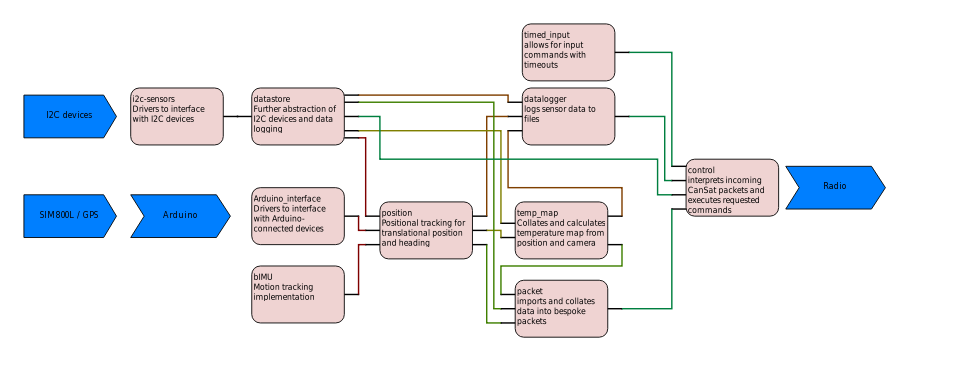
\includegraphics[scale=0.7, angle=90]{CanSat-software-diagram.png}\hspace*{\fill}
		%	\caption{The on-CanSat program structure}
		%	\label{pstruct}
		%\end{figure}
		
		\begin{sidewaysfigure}
			\centering
			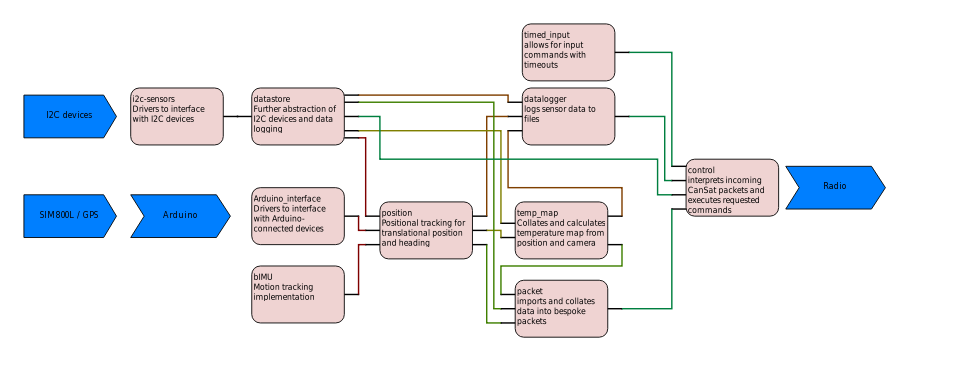
\includegraphics[scale=0.7]{CanSat-software-diagram.png}
			\caption{The on-CanSat program structure}
			\label{pstruct}
		\end{sidewaysfigure}
		
		All code used in the Linux system of the CanSat was written in Python, with a heavily customized version of Vim as a development environment. The program runs several tasks in parallel: packetization for radio transmission, data logging and backup, sensor and device control, and large-scale data processing for motion tracking and heat map creation.
		
		The base level of the program occurs inside the i2c-sensors and arduino\_interface modules. These modules abstract the raw bus interfaces for the sensors and devices present on the CanSat, enabling simple read functions and easy set functions for sensor power, update rate, and full-scale deflection. The datastore module is built on i2c-sensors and further abstracts the CanSat sensor payload into a variety of different modes. So far, the team has implemented:
		
		\begin{enumerate}
			\item min\_power: all sensors and devices aside from the Arduino, CHIP, and radio are disabled
			\item all\_active: all sensors and devices are active at full power, update, and deflection
			\item envir\_log: only sensors related to environmental data logging (humidity, temperature, and pressure) are active
			\item track\_pos: only sensors required for positional tracking (accelerometer, magnetometer, gyroscope, barometer, and GPS) are active
			\item heat\_map: only sensors required for heat map creation (accelerometer, magnetometer, gyroscope, barometer, GPS, and thermal camera) are active
		\end{enumerate}
		
		These sensor modes provide easy CanSat control, maximizing performance and battery life. The datastore module contains a variety of other features, including the ability to check sensor failure or i2c communication failure via the use of error catching code, and an implementation of functions abstracting calibration routines present in i2c-sensors.
		
		The data collected from datastore and from arduino\_interface is also used to calculate CanSat position. This is done via a Madgwick filter \footnote{http://x-io.co.uk/open-source-imu-and-ahrs-algorithms/}, which calculates accurate pitch and roll from the accelerometer and gyroscope. The accuracy of this data is further improved via a tilt-compensated magnetometer. Via these filters, the CanSat is able to accurately track its 3D orientation.
		However, translational positional tracking via accelerometer integration is prone to drift, and hence bounding sensors are necessary. This is accomplished via the barometer, from which altitude can be calculated, and the GPS, from which x-y position can be calculated to a precision of $\pm$5m.
		
		Once position and heading can be accurately calculated, the CanSat then is able to map data collected from each pixel of the thermal camera to various regions on the ground. This can be done via simple trigonometry and rotation matrices. However, in order to ensure fast update rates, pixels are assumed to represent square regions of a flat ground surface, scaled by the CanSat displacement above the ground. These algorithms are accessible in the CanSat codebase and run in a distinct thread from data logging and radio communication. 
		
		With data collected and processed from CanSat sensors, it is prepared for transmission via the packet module. The packet module, after receiving a data request from the control module, collects all required sensor data and assembles them into a packet. The contents of a packet can be arbitrarily requested and can include current sensor data points, stored sensor data points, sensor error data, positional data, and temperature maps. It is also possible to request pre-made packets with data from the modes described in datastore. Packets are also appended with a checksum, which allows the base station to confirm packet validity. Packet structure is detailed in the packet module in the CanSat codebase. 
		
		Overall CanSat control is done via the control module, which serves to interpret base station packets, change all necessary sensor settings, and instantiate a module to log data to a text file. The control module also allows for text messaging if many malformed packets are received.
		
		The Linux subsystem of the CanSat receives approximately 26kbps of data. However, much of this data is due to the high update rate for inertial sensors required for accurate positional tracking and is therefore not sent to the base station. Packets are also not sent at regular intervals: the dynamic nature of the CanSat packetization and control algorithms has led to a tested update rate of 2-5Hz over a radio link.
		
		\subsubsection{Arduino}
		Written in C++ in the Arduino IDE, the Arduino codebase is relatively simple. Via Adafruit libraries \footnote{https://learn.adafruit.com/adafruit-ultimate-gps/arduino-wiring} GPS position, speed, altitude, and validity is read from the GPS module and split into character lists, which are then transmitted to the Linux subsystem. The Arduino codebase also allows for SIM800L text messaging integration.
		
		\subsubsection{Base Station}
		The base station codebase allows easy visualization of CanSat data and overall control of the CanSat. It uses two discrete loops, one requesting data from the CanSat and the other graphing said data in a graphical user interface and providing CanSat status information. Via a set of buttons, the base station allows for sensor, power mode, and deflection settings to be constructed in packets and sent to the CanSat. The base station also performs independent data logging of received data. The base station in test mode is visible in figure \ref{bstation}, and program flow can be seen in figure \ref{bflow}.
		
		The base station code is written in Java / JavaFX within the Eclipse IDE.
		
		\begin{sidewaysfigure}
			\hfill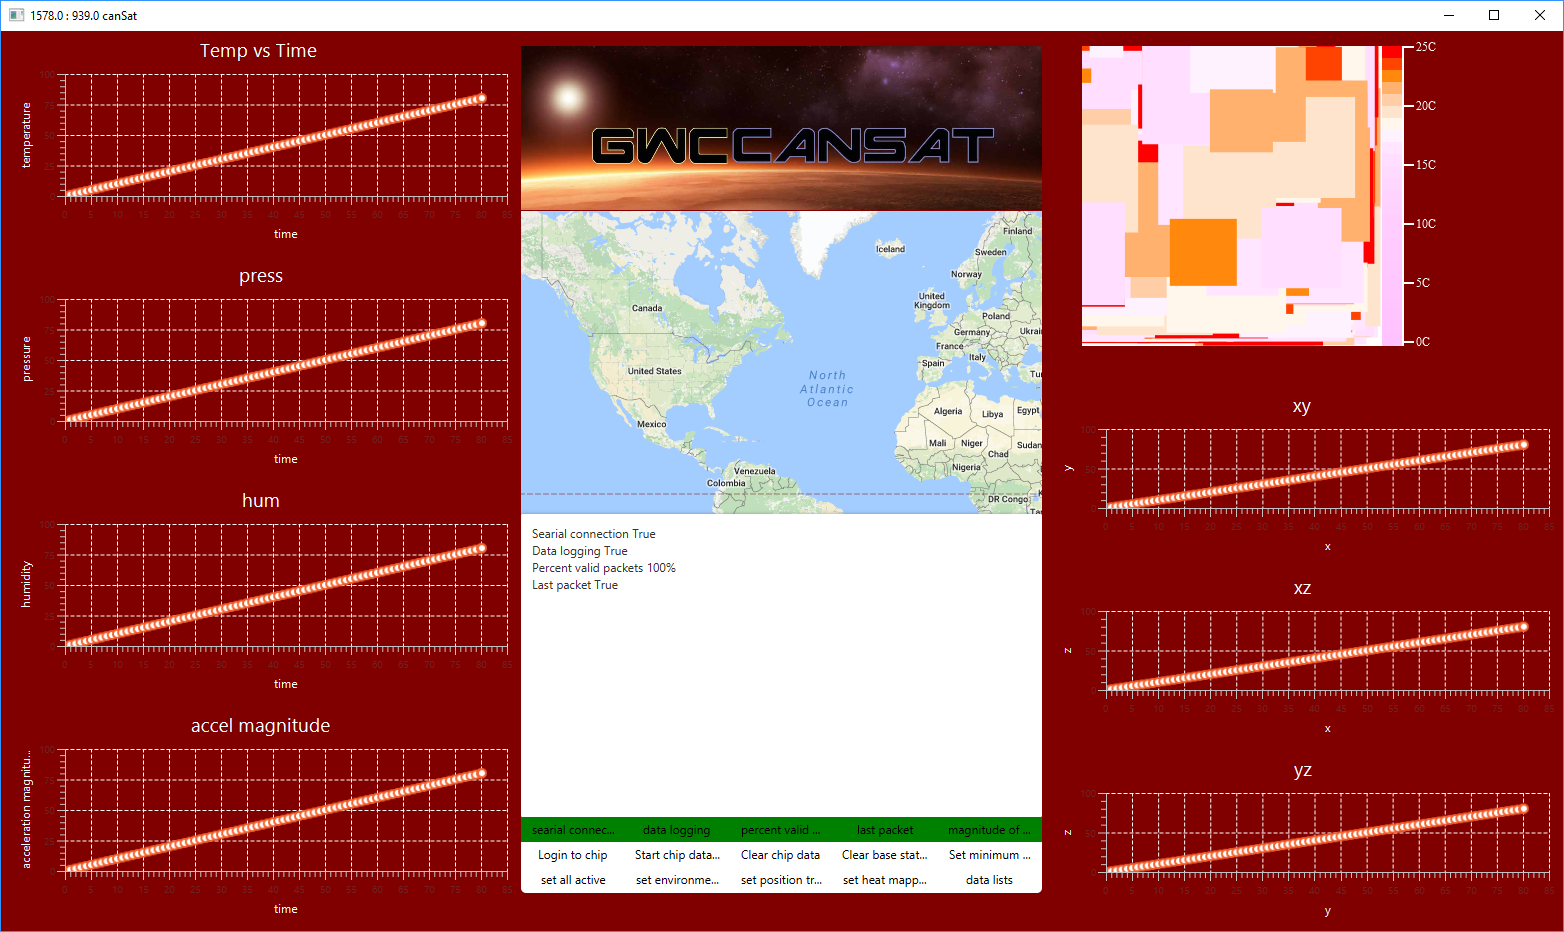
\includegraphics[scale=0.55]{base_station.png}\hspace*{\fill}
			\caption{The base station program running in test mode}
			\label{bstation}
		\end{sidewaysfigure}
		
		\begin{figure}[h]
			\hfill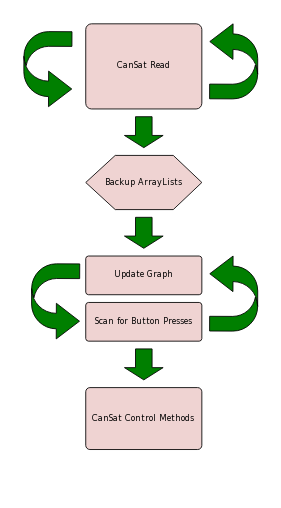
\includegraphics[scale=0.7]{Base-Station-program-flow.png}\hspace*{\fill}
			\caption{Overall flow for the base station program}
			\label{bflow}
		\end{figure}
	
	\subsection{Budget}	
	Our final CanSat budget is described below:
	\begin{center}
		\begin{longtable}{llll}
			Component Name              & Unit Price (USD) & Total Price (USD) & Price (EUR) \\ \hline
			XBEE 868LP For Europe       & n/a              & n/a               & 20.71       \\
			NTC CHIP Pro                & 16               & 16                & 14.4        \\
			Adafruit 9DOF IMU           & 19.99            & 19.99             & 17.991      \\
			Omron D6T                   & 42.9             & 42.9              & 38.61       \\
			Adafruit BME280             & 19.95            & 19.95             & 17.955      \\
			FGPMMOPA6H GPS              & 11.35            & 11.35             & 10.215      \\
			Antenna 868MHz              & 6.82             & 6.82              & 6.138       \\
			Thermal Sensor Contact      & 0.0784           & 0.3136            & 0.28224     \\
			Thermal Sensor Housing      & 0.125            & 0.125             & 0.1125      \\
			Female 5x2 Header           & 0.85             & 0.85              & 0.765       \\
			Parachute                   & 7.37             & 7.37              & 6.633       \\
			4400mAh Li-Ion battery      & 19.95            & 19.95             & 17.955      \\
			Wire (assorted)             & 5                & 5                 & 4.5         \\
			PCB (primary and secondary) & 59.12            & 59.12             & 53.208      \\
			GSM Module                  & 6.18             & 6.18              & 5.562       \\
			Plastic Frame               & 67.55            & 67.55             & 60.795      \\
			Fibreglass                  & 10               & 10                & 9           \\
			Passive Components          & 18.98            & 18.98             & 17.082      \\
			RP-SMA U.FL adapter         & 11.98            & 11.98             & 10.782      \\
			Power Switch                & 0.94             & 0.94              & 0.846       \\ \hline
			Sum:                        &                  & 325.3686          & 313.54174   \\         
		\end{longtable}
	\end{center}
	
	\chapter{Launch Campaigns}	
	\section{UK Launch Campaign: CanSat Mission}
	The UK launch campaign involved a low altitude drop of approximately 100m from a helikite \footnote{https://en.wikipedia.org/wiki/Allsopp\_Helikite}, above a field near the UK STEM Learning Center. The competition was a three day affair. The first day allowed for setup, final CanSat work, and technical inspection, the second day launch and recovery, and on the third day teams presented their CanSat, data, and analysis. After presentations had concluded, awards were given on the basis of educational value, technical achievement, teamwork, and outreach.
	\subsection{Launch Setup}
	In the second day of the competition, teams prepared their CanSats for the launch. In the case of our team launch preparation was simple. CanSat data logging was started before the CanSat was attached to the helikite, and the team's base station crew confirmed correct radio operation.
	
	\subsection{Helikite Installation}
	Suspended from the helikite was a plastic tube with a servo-controlled end cap. The prototype CanSat and parachute were loaded into the tube after data logging had begun.
	\begin{figure}[h]
		\hfill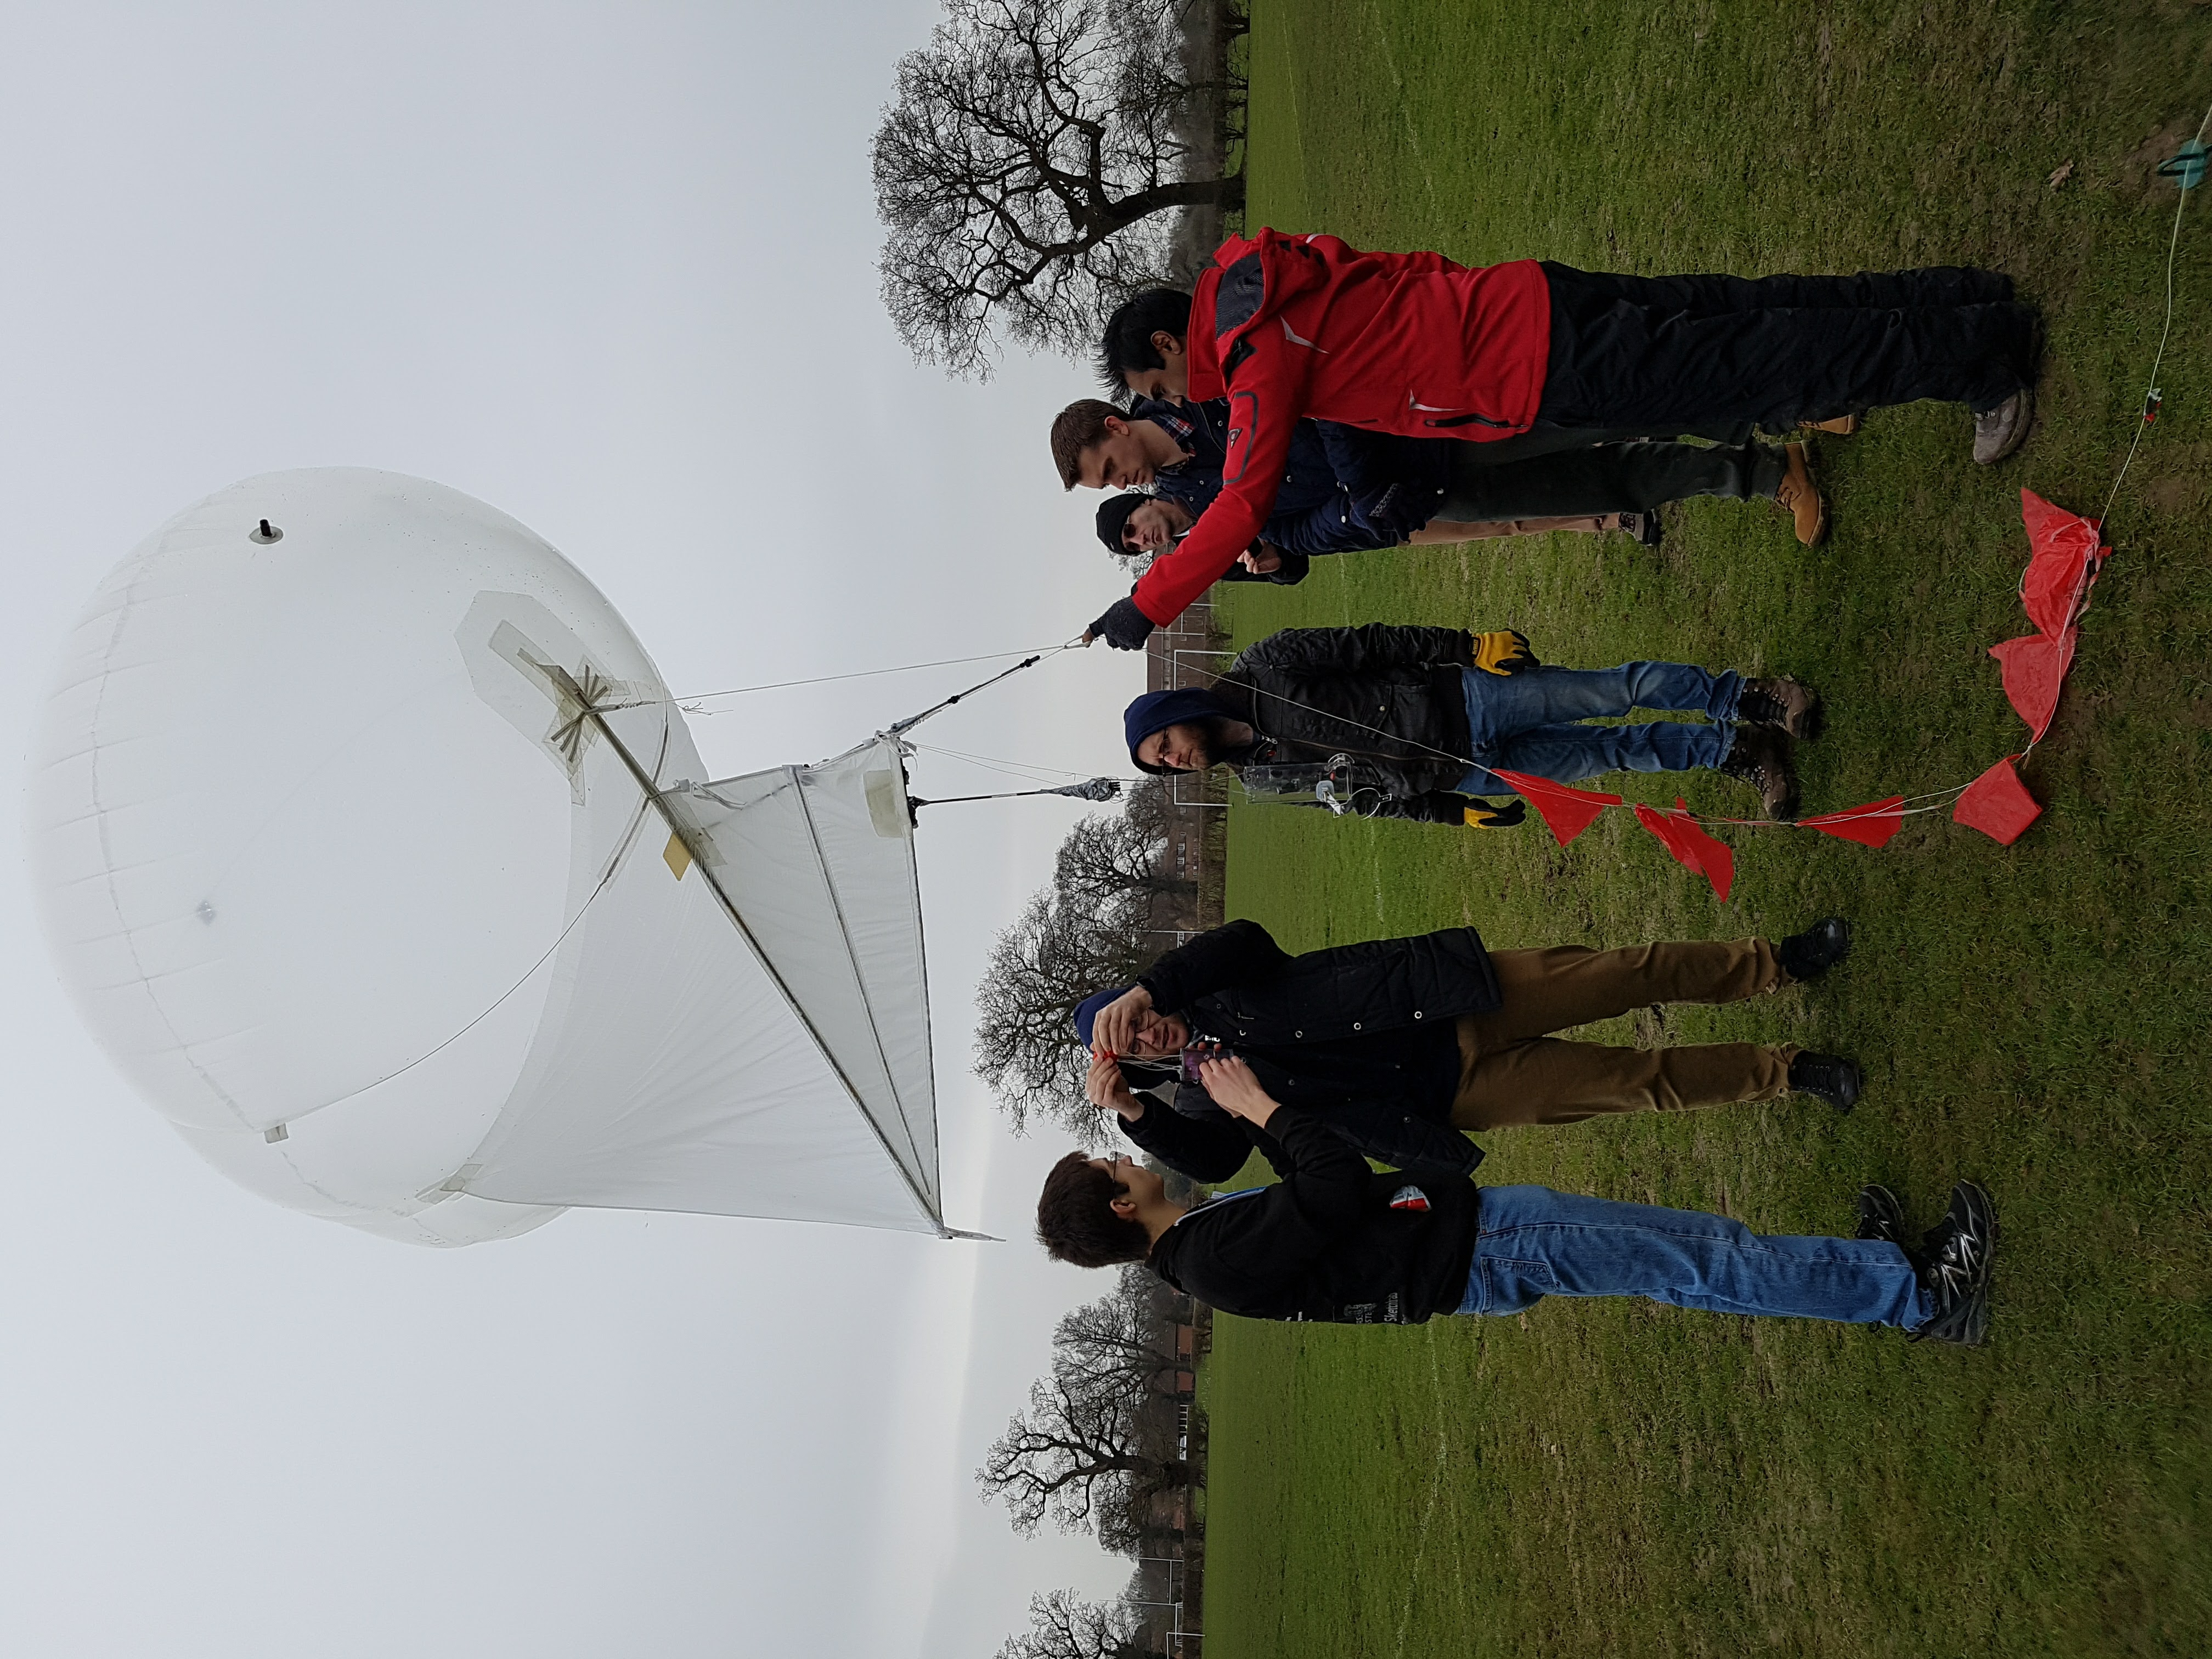
\includegraphics[scale=0.13, angle=270]{helikite.jpg}\hspace*{\fill}
		\caption{Loading the prototype CanSat in the helikite}
		\label{hkite}
	\end{figure}
	
	
	\subsection{CanSat Descent}
	Once the helikite had ascended to a peak altitude of roughly 100 meters, the launch tube released the CanSat. Large amounts of wind caused the CanSat to drift off course. However, the low drop altitude led to easy CanSat tracking.
	
	Over the course of its descent, the CanSat drifted over an agricultural field, and near landing collided with the top of a tractor. This caused no failures in the CanSat's electrical or radio subsystems, and data was able to be retrieved without issue.
	
	\subsection{Radio Performance}
	The base station lost radio contact with the CanSat at a total distance of $\approx230m$. This was due to a number of factors: misty conditions, radio band selection, and lack of antenna gain. The revised radio design in the final CanSat attempted to compensate for this.
	
	\subsection{Module Recovery}
	Due to easy visual tracking of the CanSat, GPS coordinates were not necessary to determine final CanSat location. The CanSat was retrieved by hand without issue, and the team did not observe any major damage. The collision during CanSat descent created a series of cracks in the fiberglass outer shell. However, this led to the outer shell absorbing the shock involved in the crash, thereby protecting the CanSat's sensitive electronics.
	
	\subsection{Data Recovery}
	As the CanSat logs sensor data at very high update rates, the team decided to recovery data via a USB flash drive. The drive was mounted by means of a USB-A port on the CHIP, and log files in text format were transferred to the drive.
	
	
	\section{UK Launch Campaign: Data Analysis}
	After processed and logged data had been recovered via a USB flash drive, it was further processed via Microsoft Excel. A complete dataset, not including thermal camera imagery, can be found at a separate GitHub repository \footnote{github.com/arcturus314/cansat2017\_data}.
	
	\subsection{Primary Mission: Temperature and Pressure}
	
	\begin{figure}[h]
		\hfill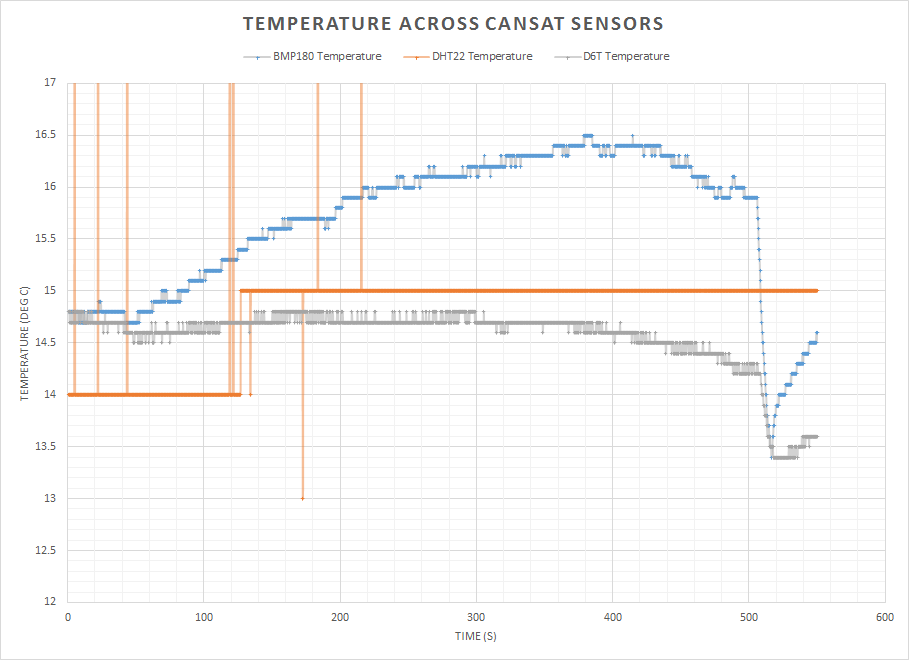
\includegraphics[scale=0.7]{temps.png}\hspace*{\fill}
		\caption{Temperature sensors within the prototype CanSat throughout its mission}
		\label{ptemps}
	\end{figure}
	
	The graph in figure \ref{ptemps} indicates substantial temperature rise throughout the CanSat descent. This clearly should not be the case, and indicates a transfer of thermal energy from the CHIP CPU, which generates a substantial amount of heat, to sensors within the CanSat. It is still possible to observe the atmospheric temperature to be $\approx14.7\degree C$ via the D6T, which remained exposed to substantial airflow.
	
	Pressure follows the expected trend, decreasing by approximately 15hPa throughout the CanSat descent. Pressure extrapolated to relative altitude can be seen in figure \ref{palt}, and indicates that the total drop distance was 120m with an average descent rate of $10.5ms^{-1}$. 

	\begin{figure}[h]
	\hfill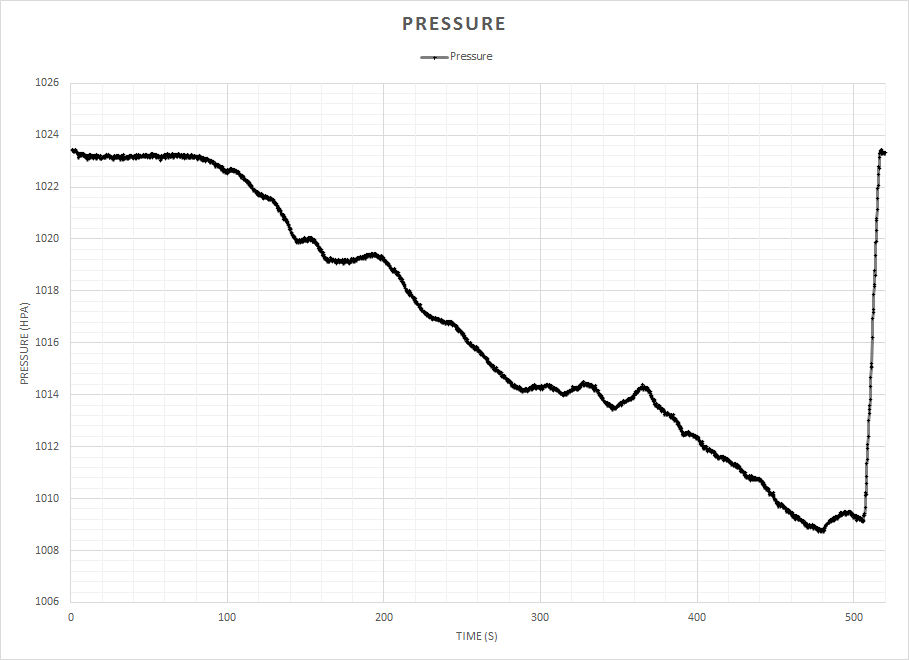
\includegraphics[scale=0.7]{pressure.png}\hspace*{\fill}
	\caption{Atmospheric pressure measured by the prototype CanSat throughout its mission}
	\label{ppres}
	\end{figure}

	\begin{figure}[h]
	\hfill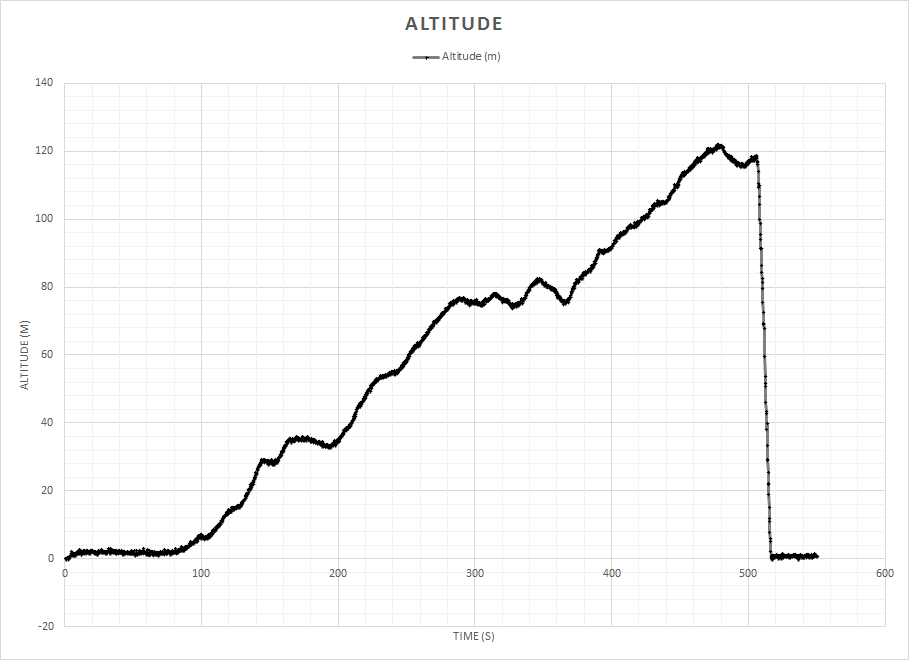
\includegraphics[scale=0.7]{altitude.png}\hspace*{\fill}
	\caption{Calculated prototype CanSat altitude throughout its drop}
	\label{palt}
	\end{figure}
	
	The team identified the start and end of the CanSat descent via a graph of accelerometer magnitude (calculated via $a_t = \sqrt{a_x^2 + a_y^2 + a_z^2}$). The graph indicates substantial spikes and instability in the region of 506s-517.5s. Therefore the team deduced this region to be that of CanSat release, descent, and landing.
	
	\begin{figure}[h]
		\hfill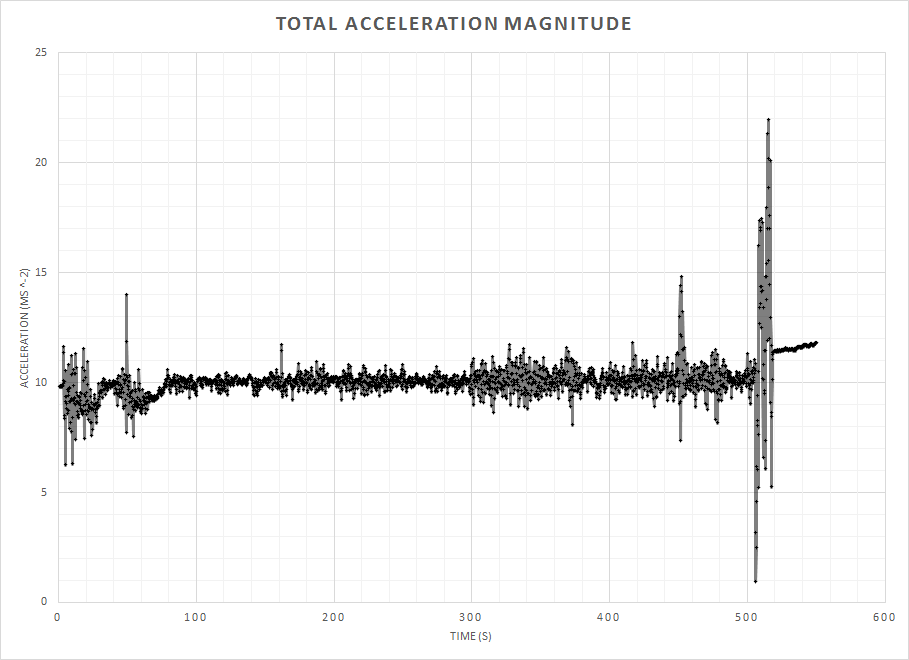
\includegraphics[scale=0.7]{accel_mag.png}\hspace*{\fill}
		\caption{Acceleration throughout the CanSat descent}
		\label{accel}
	\end{figure}
	
	The team experienced issues with the humidity sensor and its associated temperature sensor. Relative humidity can be seen in figure \ref{hum}, however, it is clear that the sensor ceased to update approximately 200 seconds into the CanSat flight. Unfortunately, this prevents us from examining trends related to atmospheric humidity.

	\begin{figure}[h]
	\hfill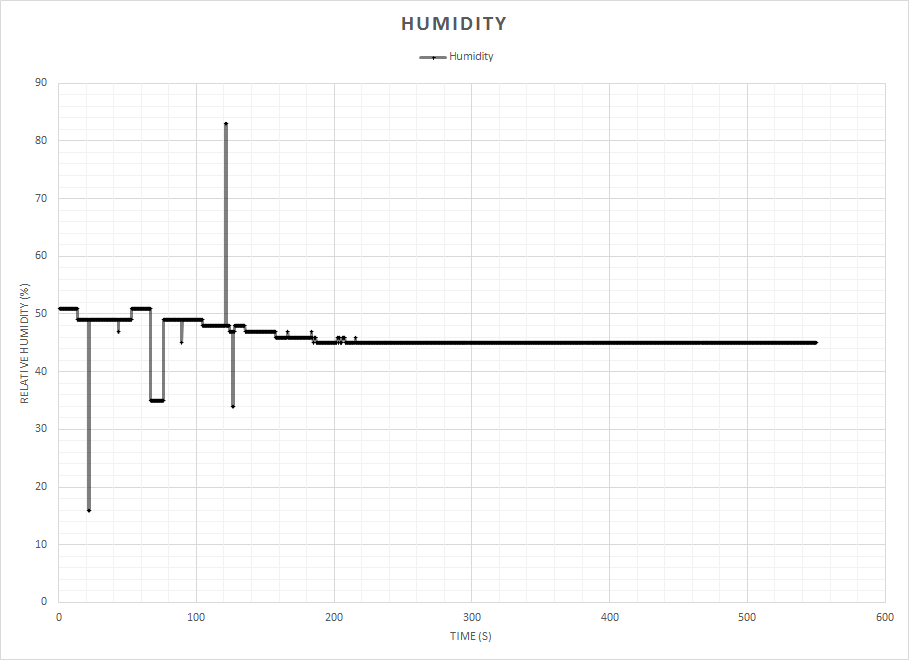
\includegraphics[scale=0.7]{humidity.png}\hspace*{\fill}
	\caption{Measured humidity through prototype CanSat descent}
	\label{hum}
	\end{figure}
	
	\subsection{Secondary Mission: CanSat Motion}
	
	Examination of gyroscope and magnetometer values during descent, seen in figure \ref{pimu}, indicated substantial vibration, something also seen while watching the CanSat descent. Gyroscope values were integrated to produce a rough approximation of CanSat orientation. However, this methodology proved to be flawed: without a more robust, multi-sensor mechanism of orientation tracking calculated orientation values were subject to substantial drift. The team solved this issue in the final CanSat through use of a Madgwick sensor fusion algorithm.
	
	In the final CanSat, the full scale deflection of the gyroscope was also increased.
	
	\begin{figure}
		\centering
		\begin{subfigure}{.5\textwidth}
			\centering
			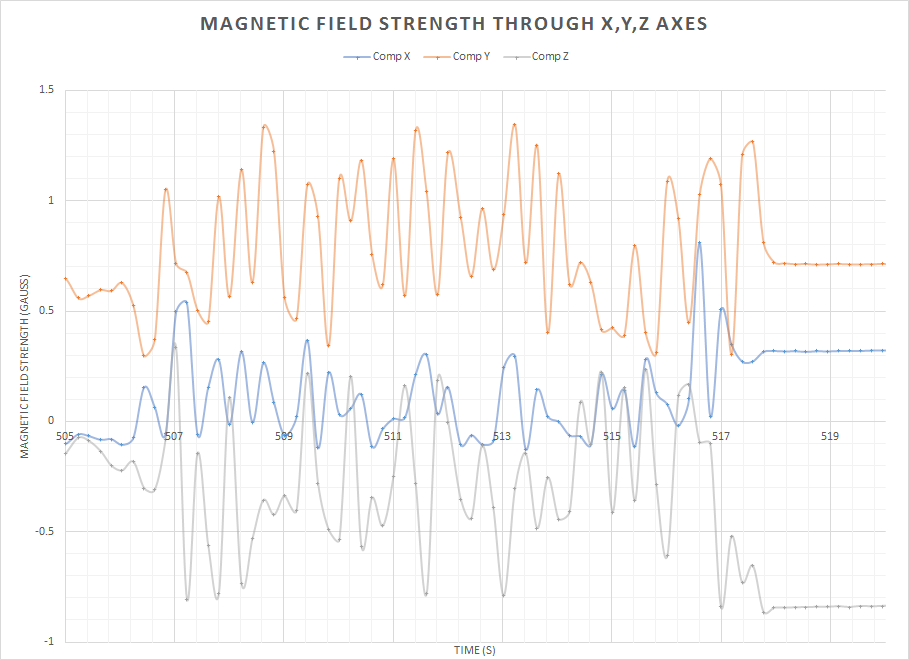
\includegraphics[width=1\linewidth]{mag.png}
		\end{subfigure}%
		\begin{subfigure}{.5\textwidth}
			\centering
			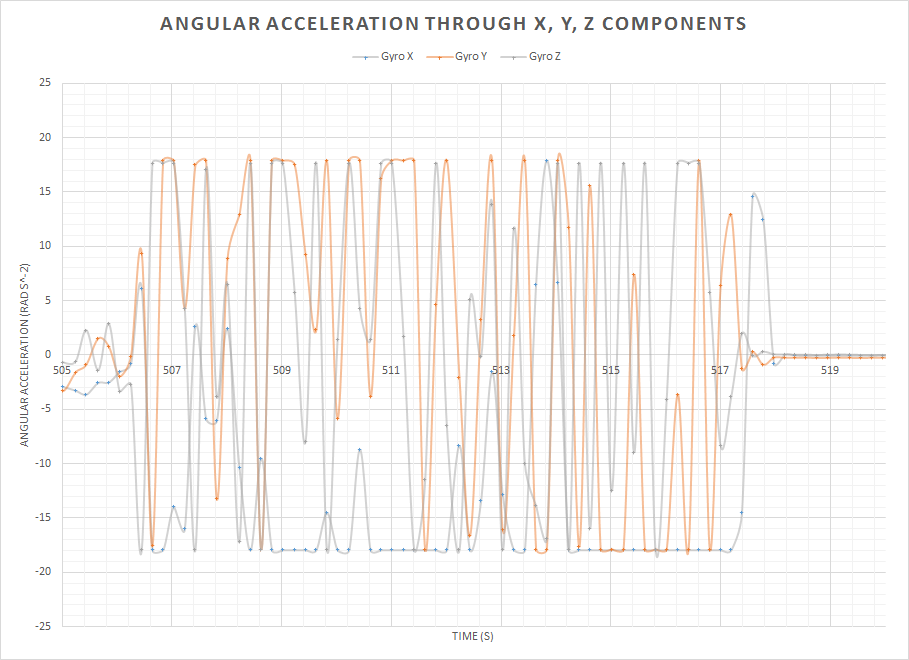
\includegraphics[width=1\linewidth, angle=0]{gyro.png}
		\end{subfigure}
		\caption{IMU data over the prototype CanSat mission}
		\label{pimu}
	\end{figure}

	It was also necessary to produce a rotation-compensated temperature matrix value. This was simply done via a two-dimensional rotation matrix, which can be seen in equation \ref{eq1}. 
	
	\begin{center}
	\begin{equation} \label{eq1}	
	\begin{bmatrix}
	\cos\theta & -\sin\theta \\
	\sin\theta & \cos\theta
	\end{bmatrix}	
	%\quad
	\begin{bmatrix}
	t_{x0} & t_{x1} & t_{x2} & . . . & t_{x12} & t_{x13} & t_{x14} & t_{x15} \\
	t_{y0} & t_{y1} & t_{y2} & . . . & t_{y12} & t_{y13} & t_{y14} & t_{y15}
	\end{bmatrix}
	\end{equation}
	\end{center}

	These motion tracking features were the extent of our motion-based secondary mission in the prototype CanSat. 
	
	\subsection{Secondary Mission: Heat Map}
	
	The CanSat logged a sixteen pixel image from the thermal camera every update interval. The offset of each pixel was used as $(t_{xn}, t_{yn})$ coordinates in the data matrix post-multiplying the rotation matrix that was seen in equation \ref{eq1}.
	
	Thermal mapping data appeared as expected. Unfortunately, at a 100m drop distance, no interesting atmospheric features such as clouds could be identified, and the grassy field the CanSat was dropped over did not exhibit any noteworthy thermal features. Our algorithm performed suitably, providing a almost-uniform temperature over its recording.
		
	\section{EU Launch Campaign: CanSat Mission}
	
	The European competition functioned as a higher level, extended version of the UK competition. After an introductory ceremony on the first day, teams were accompanied to an air field for technical inspection, drop tests, and launches on the second and third day. The technical portion of the competition was followed with presentations and awards on the fourth, final day. 
	
	In this final competition, CanSats were dropped via a Quest Intruder model rocket \footnote{http://www.sierrafoxhobbies.com/en/high-power-rockets/484-rocket-kit-intruder-public-missiles-ltd.html}. 
	
	All recovered mission data is, as before, available at a team GitHub repository \footnote{github.com/arcturus314/cansat2017\_data}.
	
	\subsection{Launch Setup}
	
	Prior to the launch, the team began data logging on the CanSat. This was because misty weather conditions would cause reduced radio range, and the team wanted to ensure that the CanSat would collect data during the descent period. Following base station setup and CanSat activation, the CanSat was taken to the launch site by car, approximately 1km away from the base station and hangars.
	
	The CanSat was installed as one of three units within the Intruder rocket. Figure \ref{rocket} illustrates CanSat installation. After the rocket technician had installed the CanSats and prepared the rocket, the launch party, composed of one member representing each CanSat during the launch, was led into a car a distance away from the launch.
	
	\begin{figure}[h]
		\hfill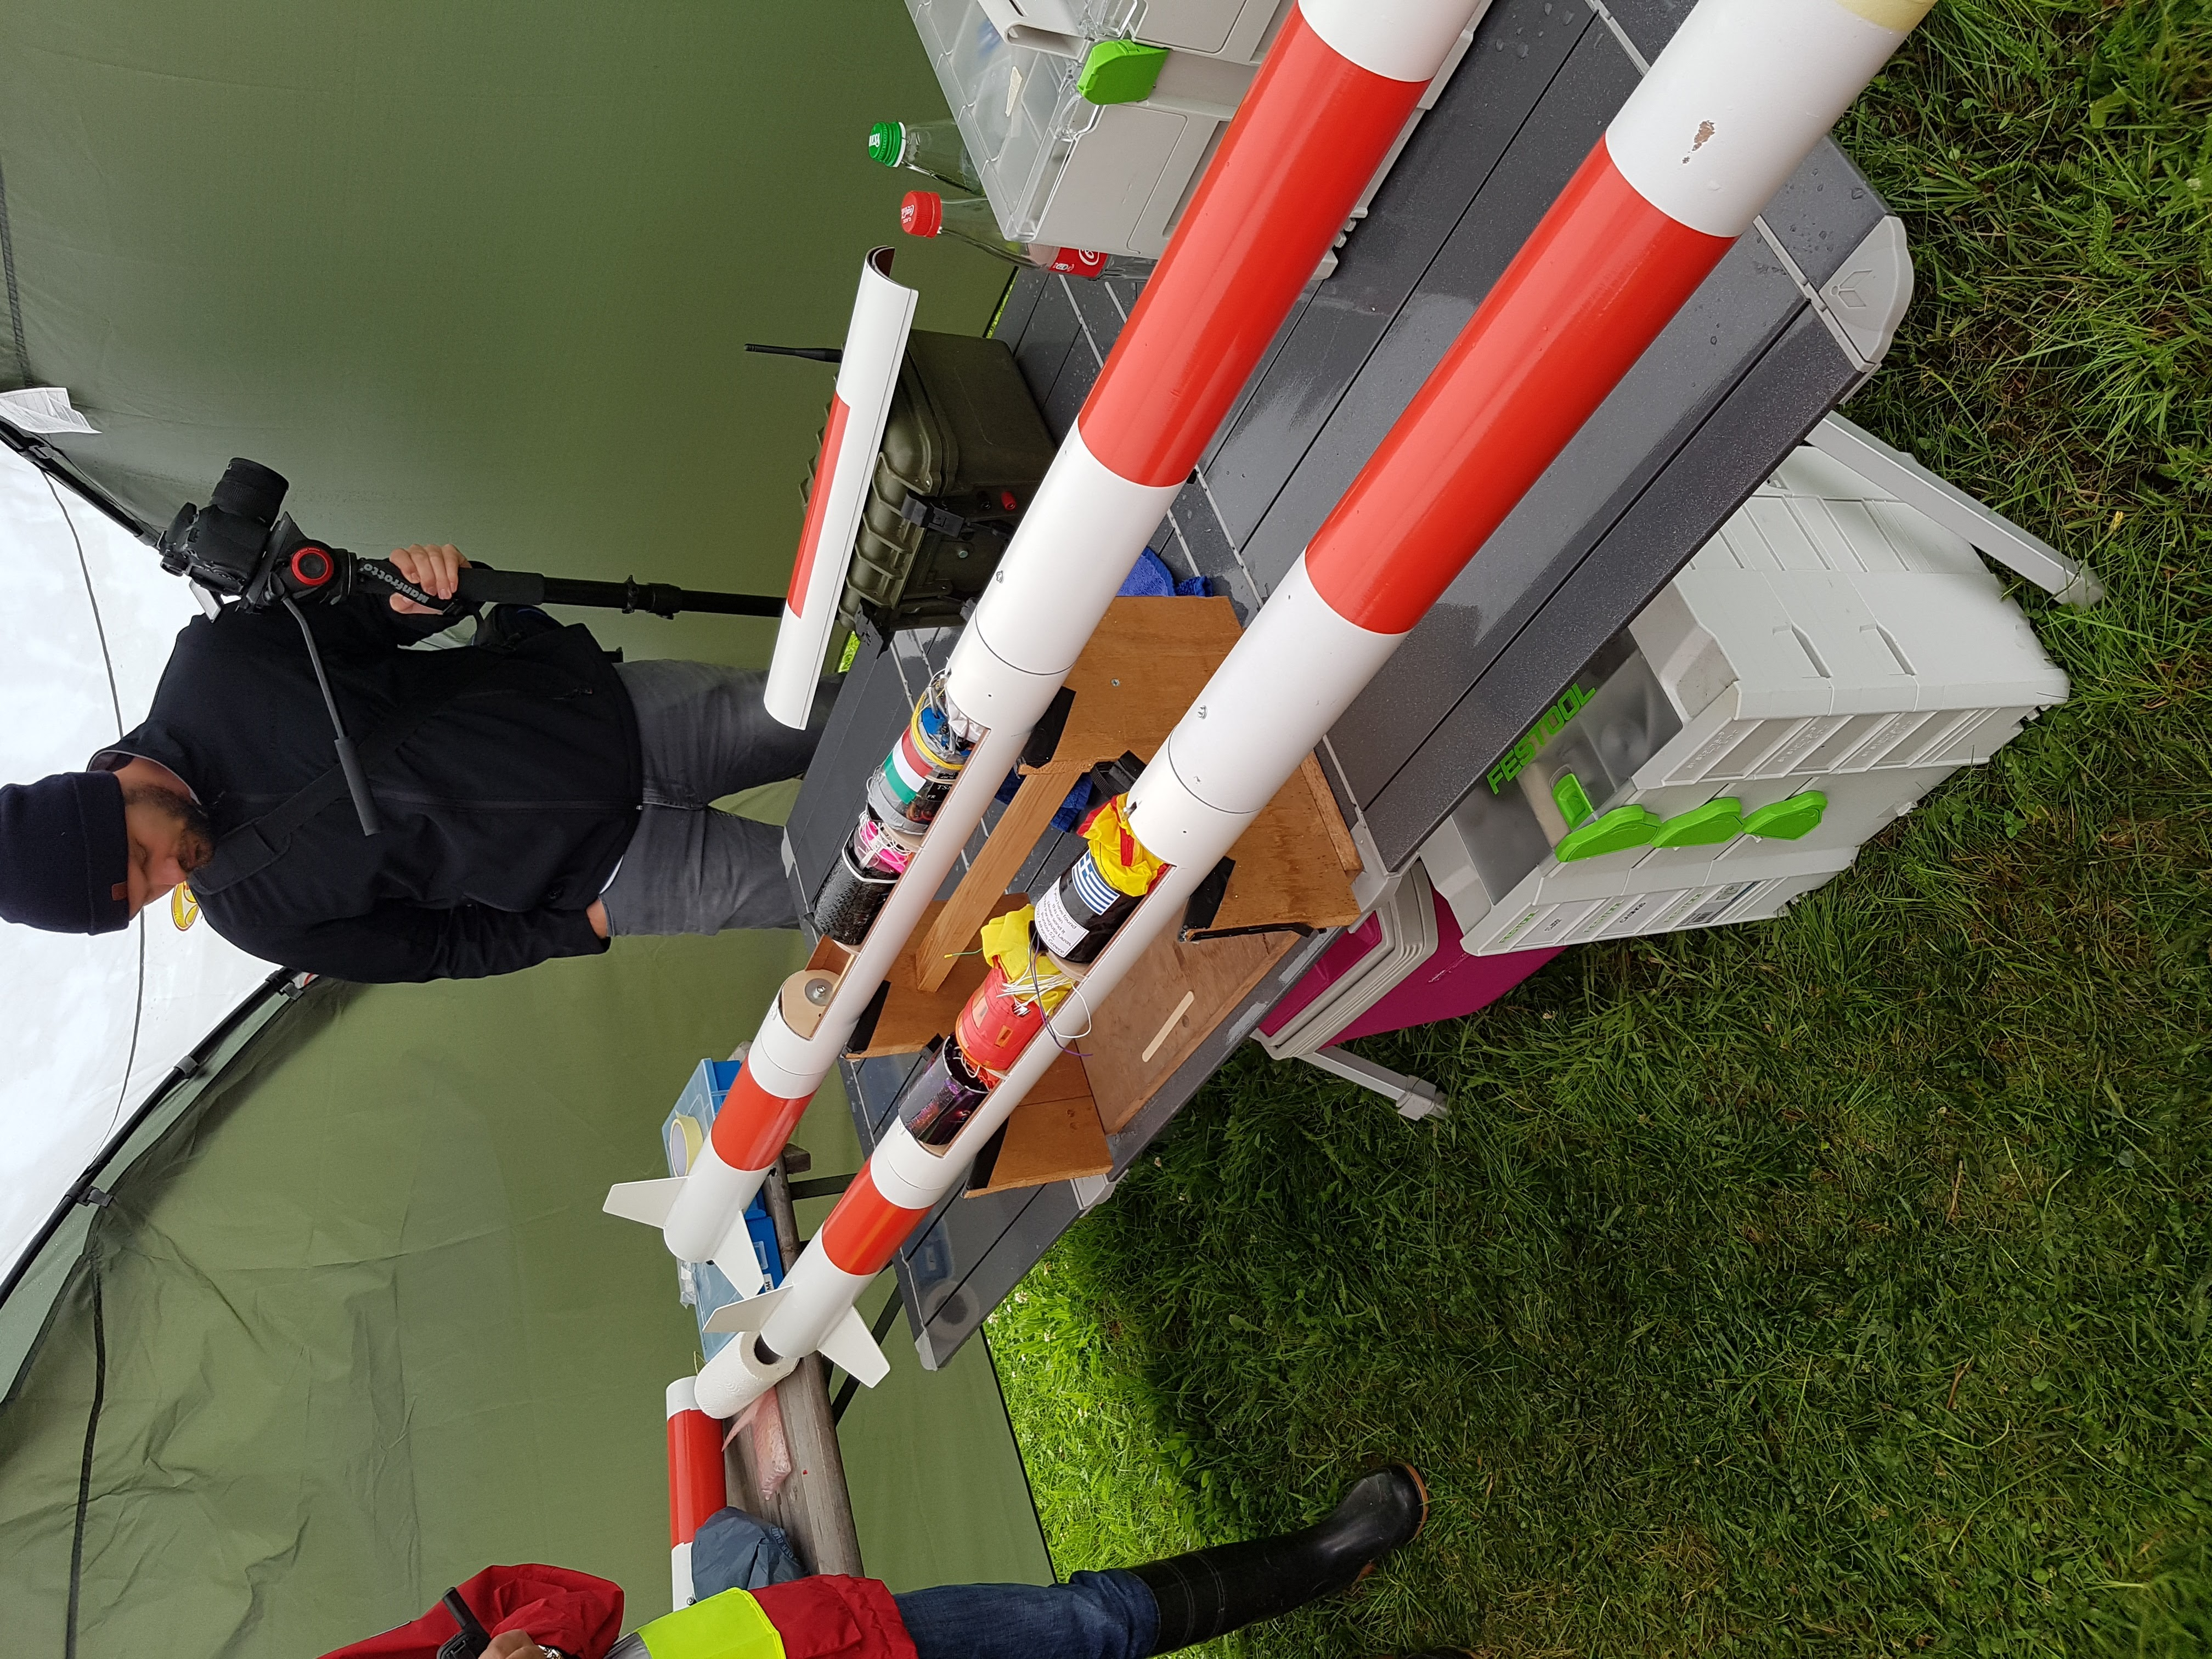
\includegraphics[scale=0.1, angle=270]{rocket_load.jpg}\hspace*{\fill}
		\caption{Loading our CanSat into the rocket, in position closest the rocket motor}
		\label{rocket}
	\end{figure}
	
	
	\subsection{Rocket Launch and Descent}
	
	After launch, the rocket immediately began to drift off course, which can be seen in figure \ref{rlaunch}. This continued through the flight of the rocket: it was due to sudden gusts of wind, and carried our module farther from the hangars and base station. The team was not able to observe CanSat release due to cloud cover. However, the CanSat had descended into a patch of forest and swamp, exacerbated by the rainy conditions of the past few days.
	
	\begin{figure}[h]
		\hfill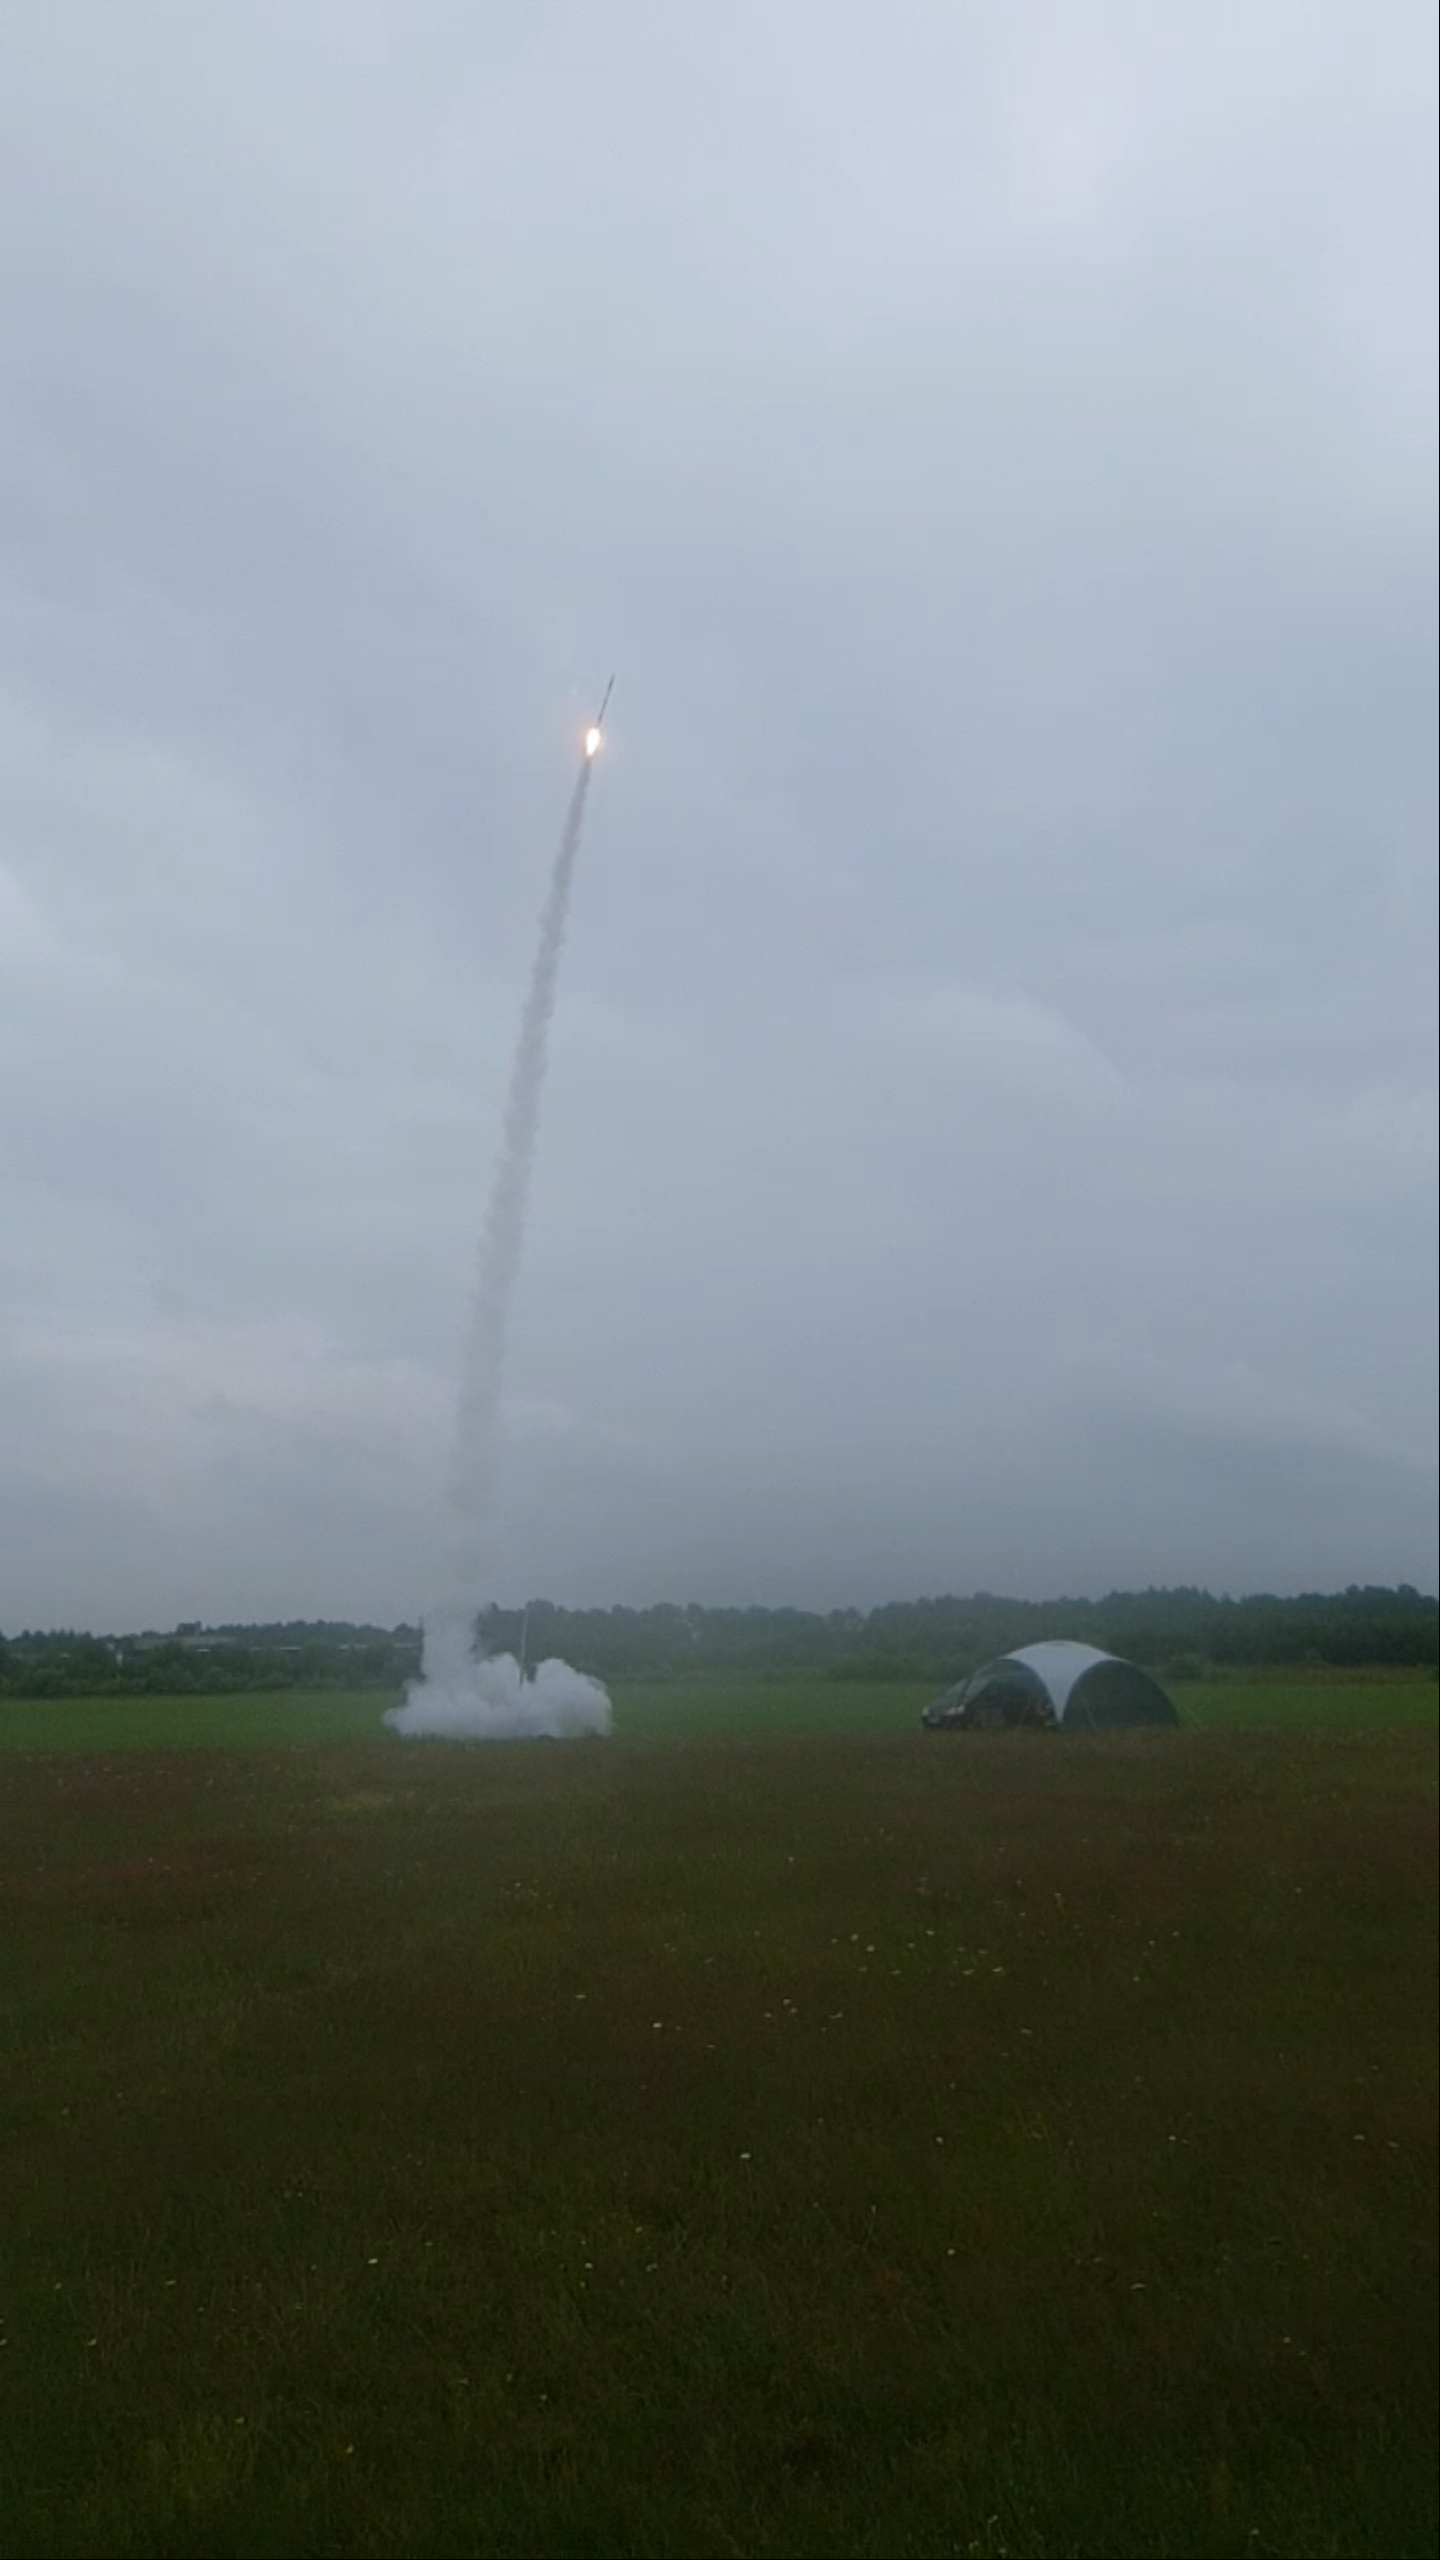
\includegraphics[scale=0.25]{rlaunch.png}\hspace*{\fill}
		\caption{The launch vehicle's ascent}
		\label{rlaunch}
	\end{figure}
	
	\subsection{Radio Performance}
	
	The base station was neither able to begin or hold a successful radio link after the CanSat had launched. The team believes this to be due to a number of factors:
	
	\begin{enumerate}
		\item \textbf{Rocket drift.} The launch rocket did not follow the expected path, instead blown away from the team's base station due to weather conditions. This furthered the range our radio needed to cross, leading to connectivity issues. \\
		\item \textbf{Misty weather conditions.} Through the day of the launch, there was high atmospheric relative humidity, and the launch site proved to be very misty. Unfortunately, water is a fantastic absorber of electromagnetic radiation, and likely reduced our effective radio range. \\
		\item \textbf{CanSat mechanical design changes.} The team elected to use steel internal frame top pieces in our design to increase parachute mounting point strength, as the team was concerned about parachute lines shearing through our plastic mount. However, these internal frame pieces may have interfered with radio range.
	\end{enumerate}

	\subsection{Module Recovery}
	
	Due to the module's location on landing, it was impossible to recover. GWC CanSat would like to thank Spain's CanSat team, \textit{La Burgoneta Espacial}, for their assistance in the search for our CanSat. 
	
	The team was able to locate CanSat position to a 50m x 50m area via GPS- a picture was taken of the rough location, and from there find a position, seen in figure \ref{dl} that allowed stable radio link.
	
	\begin{figure}[h]
		\hfill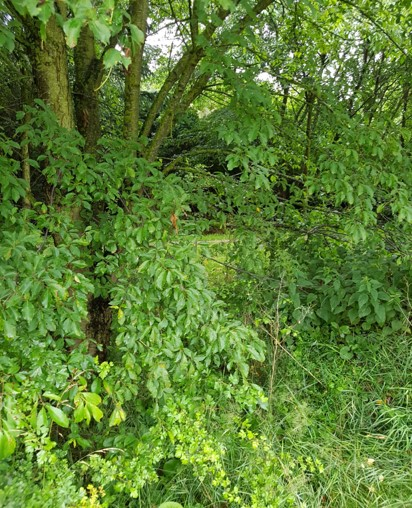
\includegraphics[scale=1.2]{cloc.jpg}\hspace*{\fill}
		\caption{An image of the CanSat landing site. The team believes that the CanSat is stuck on top of tree cover}
		\label{cloc}
	\end{figure}

	\begin{figure}[h]
	\hfill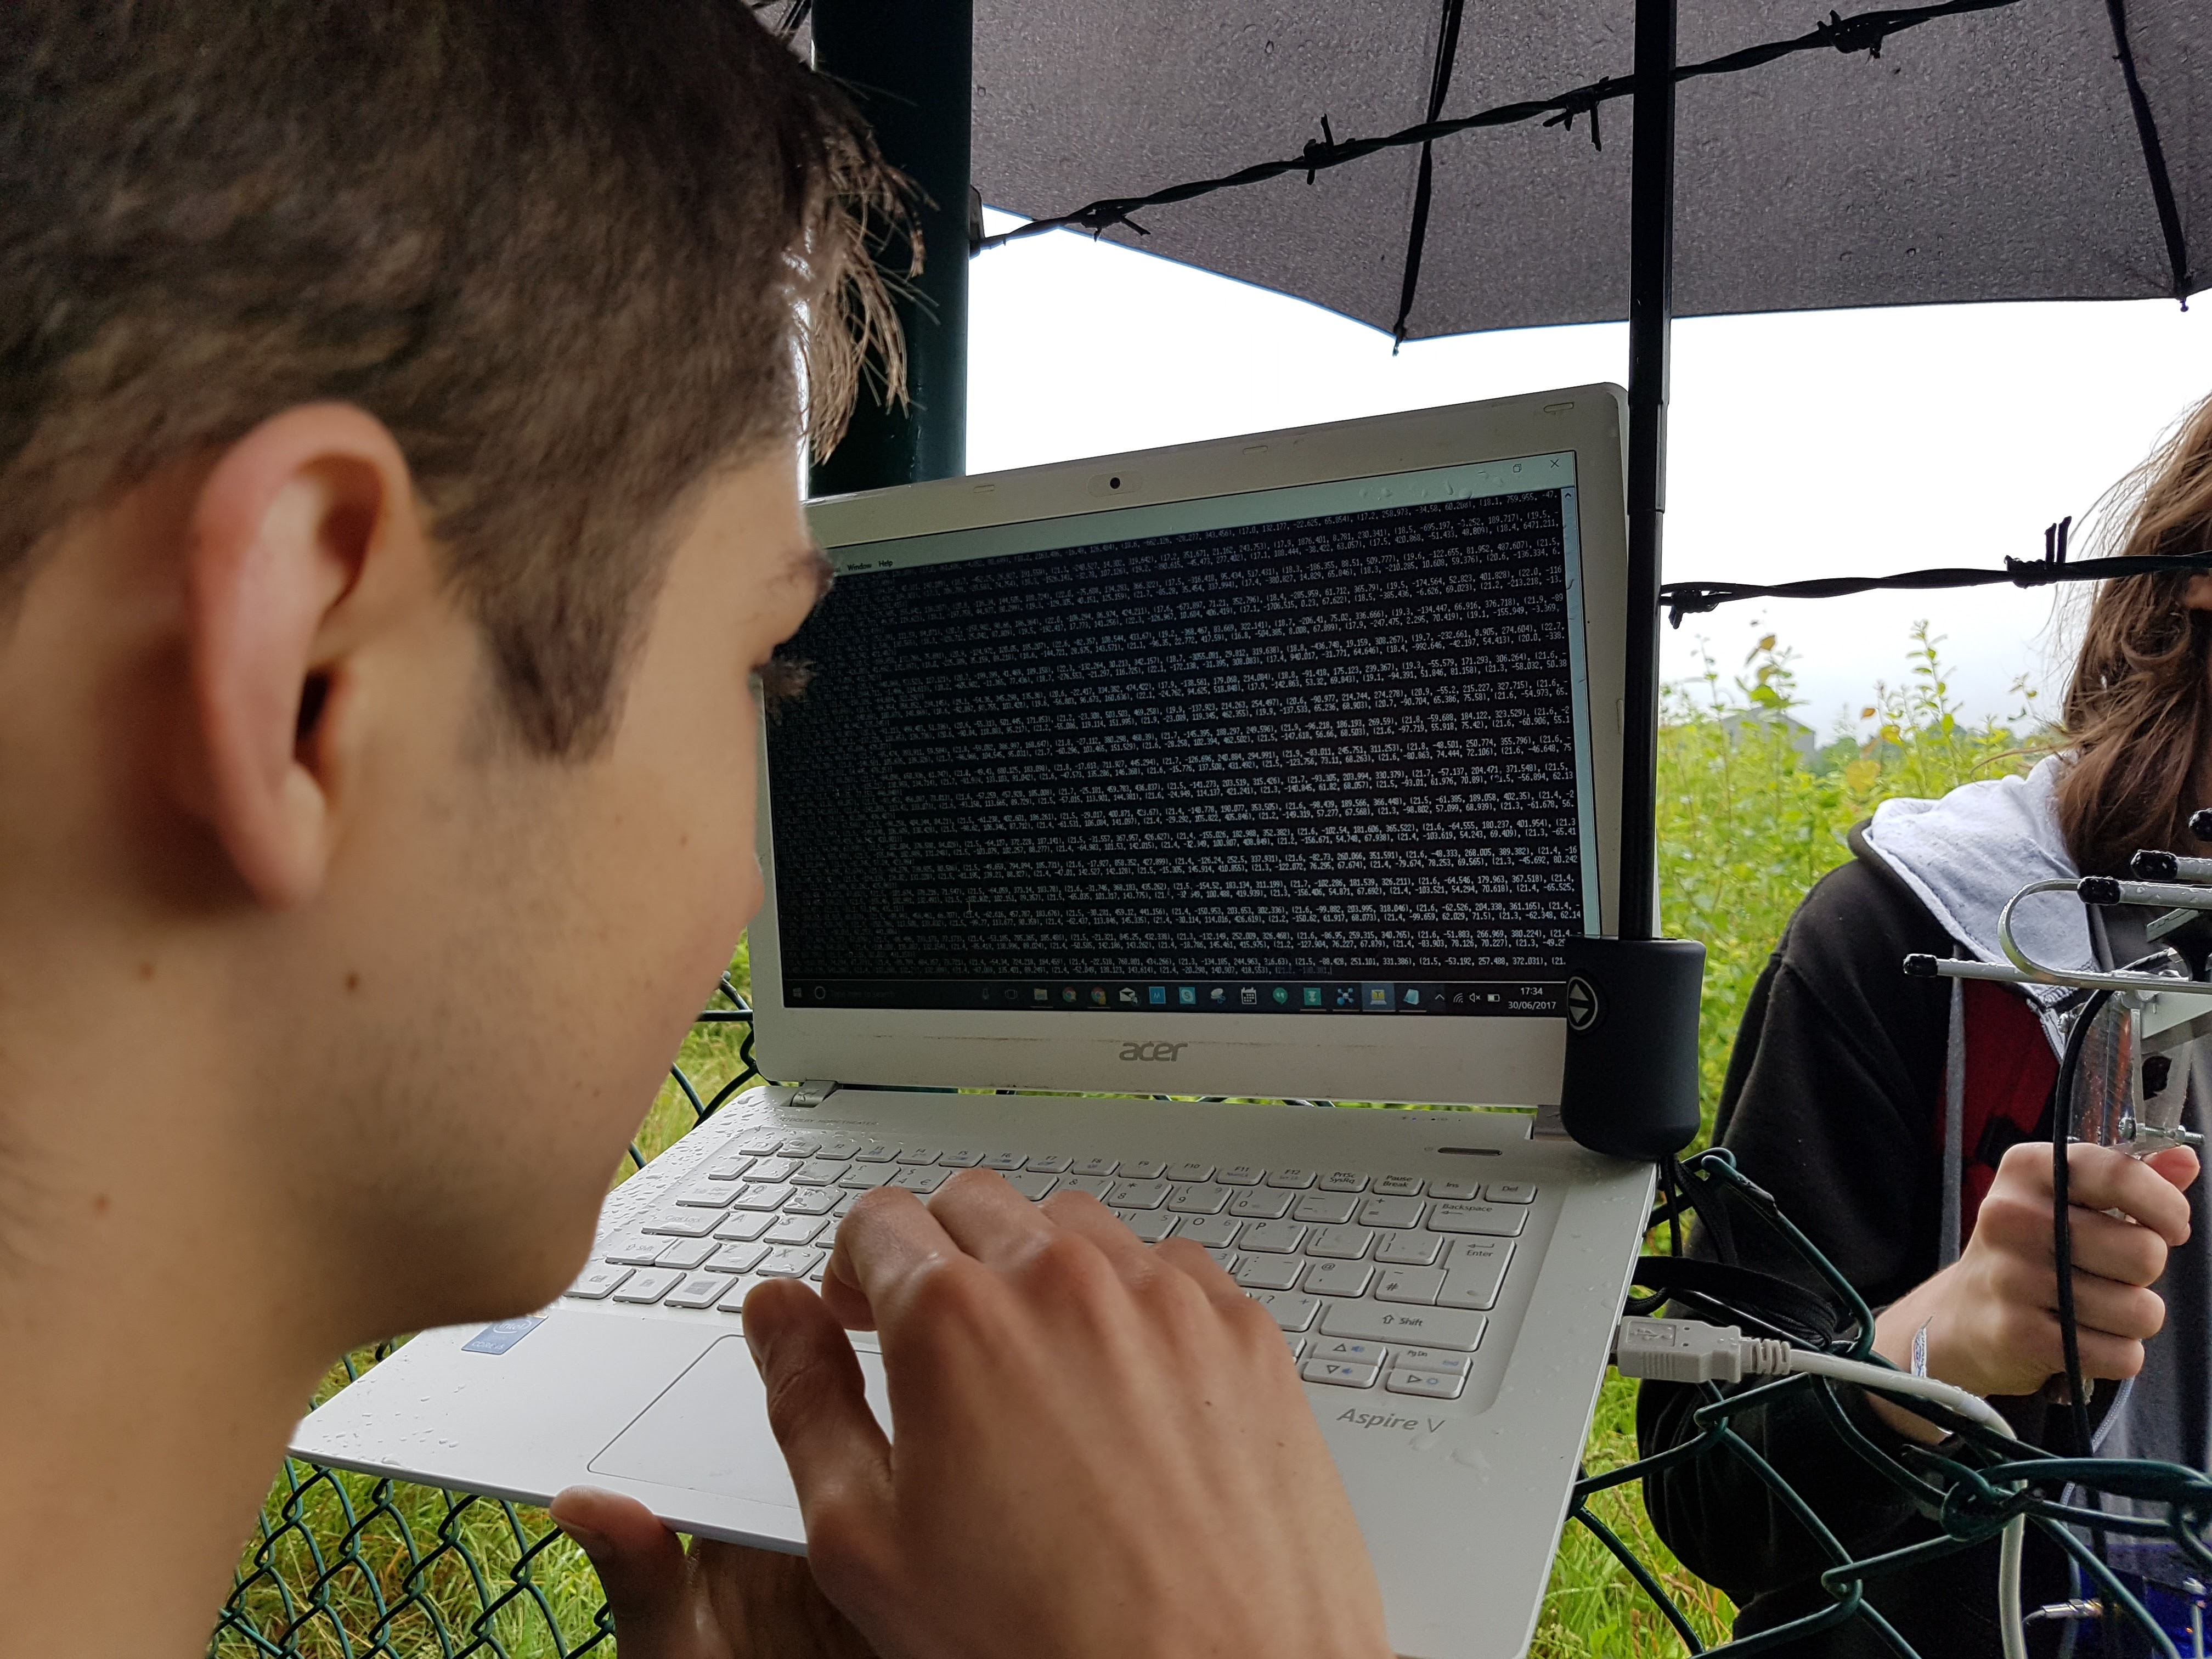
\includegraphics[scale=0.13]{retrieval.jpg}\hspace*{\fill}
	\caption{Downloading data from the CanSat}
	\label{dl}
	\end{figure}
	
	\subsection{Data Recovery}
	
	After obtaining stable radio link with the CanSat, it was possible for the search party to begin data download. As our radio architecture presents the base station with a Linux terminal accessible on the CanSat, it was possible to use native Linux commands: ex \textit{cat filename.txt $>$ tty/terminal name} to echo the contents of a file to the terminal, where it would appear printed on the base station screen.
	
	Via this method the team was able to retrieve some data from the CanSat. However, due to our high data logging rate, and the relatively slow 9600 baud radio connection, data download was slow. Additionally, the team had very limited time in which to download data. Therefore only 0.6\% of the total data set was retrieved.
	
	\section{EU Launch Campaign: Data Analysis}
	Despite the loss of the CanSat and of the majority of the team's dataset, we regard our CanSat's mission as a success. The module functioned without issue during descent and landing, and from the limited data received appeared to accurately fulfill both its primary and secondary missions.
	
	\subsection{Primary Mission}
	
	Unfortunately, the datafile containing stored primary mission data begun to fill as soon as data logging began. Hence, all of our recovered data is of the time period in which the CanSat was transported from the hangars to the launch site. This hypothesis is supported via visualization of recovered temperature, pressure, and humidity data. It is important to note that the temperature graph plotted here is of the mean between the temperature sensor embedded in the D6T and BME280: the L3GD20 was positioned near the CHIP Pro, which becomes quite warm during use, leading to skewed temperature readings. This was predicted in our design- it's what led us to position other temperature sensors throughout the CanSat. Visualized pressure, temperature, and humidity data is available in figures \ref{rh}, \ref{rt}, and \ref{rp}.
	
	\begin{figure}[h]
		\hfill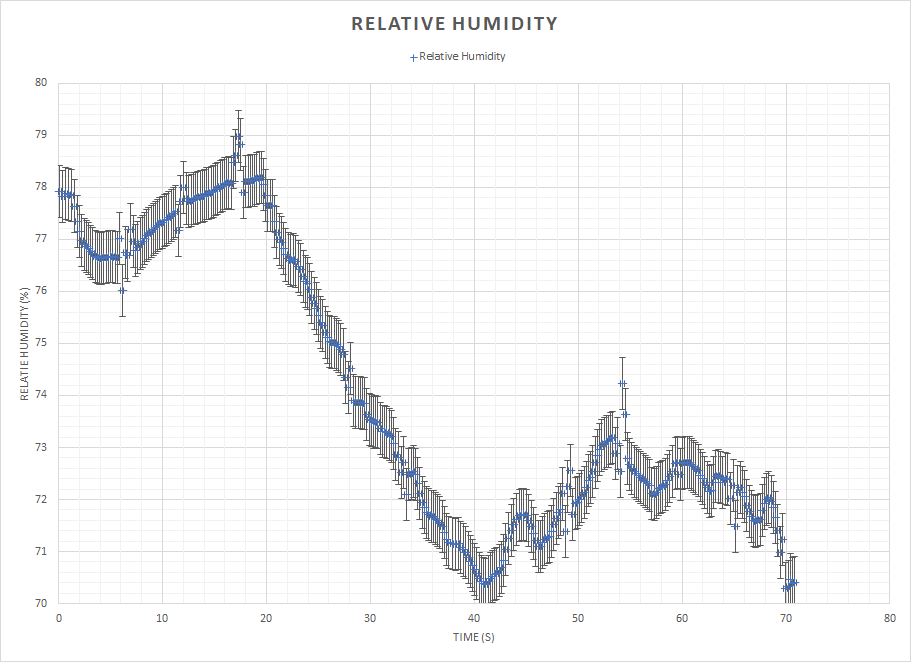
\includegraphics[scale=0.7]{hum_fin.png}\hspace*{\fill}
		\caption{Retrieved humidity data}
		\label{rh}
	\end{figure}

	\begin{figure}[h]
		\hfill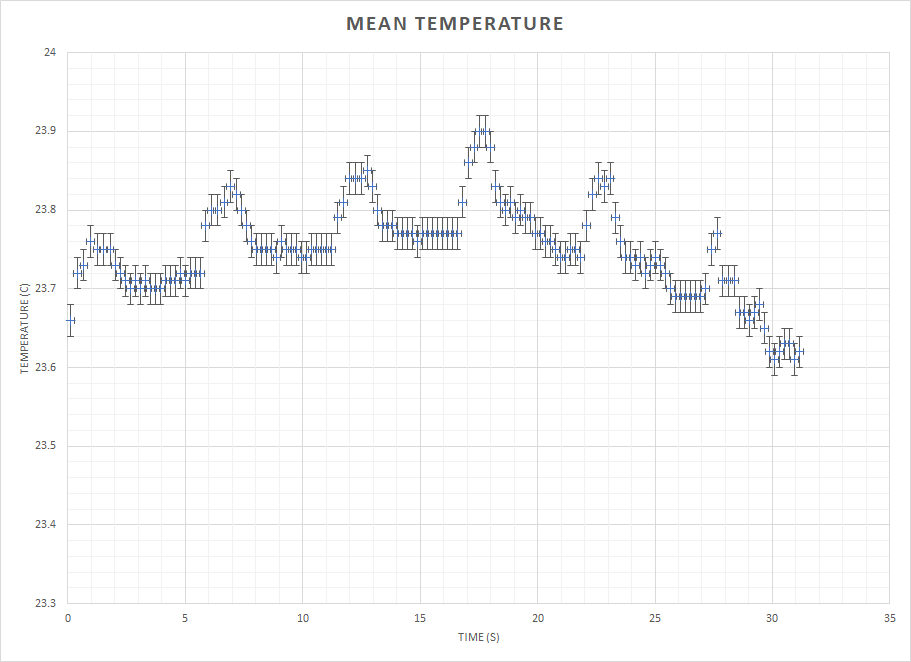
\includegraphics[scale=0.7]{temp_fin.png}\hspace*{\fill}
		\caption{Retrieved temperature data}
		\label{rt}
	\end{figure}

	\begin{figure}[h]
		\hfill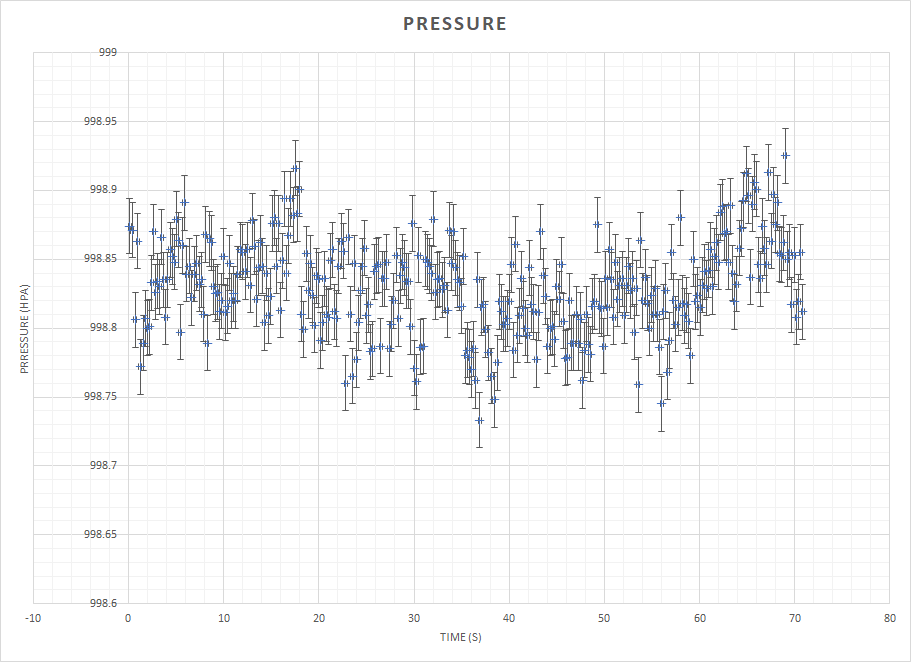
\includegraphics[scale=0.7]{pres_fin.png}\hspace*{\fill}
		\caption{Retrieved pressure data}
		\label{rp}
	\end{figure}

	While the given pressure data shows nothing besides random noise, there are clear features in both humidity and pressure data. The large drop seen in the humidity data is due to a team member breathing into the CanSat during the trip to the launch site: this provides the team with a clear reference point and timestamp. The periodic temperature increases in temperature data are simply due to shifts in the CanSat position- it was passed between a team member's hands in a periodic motion.
	
	Unfortunately, the small amount of recovered data led to difficulties in identification of any useful trends.
	
	\subsection{Secondary Mission}
	
	Many data processing layers are used on-CanSat to construct a heat map from raw sensor data. These include orientation tracking, x-y positional tracking, and pixel location tracking.
	
	Orientation tracking relies on a Madgwick algorithm, which the team customized and optimized for the large amount of processing power on the CanSat. While the algorithm itself is very complex, our implementation can be seen at the team GitHub \footnote{github.com/arcturus314/cansat2017} in \textit{MadgwickAHRS.py}, and the original paper is available at \footnote{http://x-io.co.uk/res/doc/madgwick\_internal\_report.pdf}.
	
	Translational position tracking proved to be less difficult. The CanSat first converts accelerometer X, Y, and Z components into components along a fixed heading, to allow for consistent integration along vectors with the Earth as a reference plane, seen in equations \ref{eq2} and \ref{eq6}.
	
	\begin{equation} \label{eq2}
	accel_{xcomp}=(accel_y\times\cos heading + accel_x\times\sin (heading))\times\sin xtilt 
	\end{equation}
	\begin{equation} \label{eq6}
	accel_{ycomp}=(accel_y\times\sin heading + accel_x\times\cos (heading))\times\sin ytilt
	\end{equation}
	
	Accelerometer data was then integrated through a trapezoidal method, seen in equation \ref{eq3}
	
	\begin{equation} \label{eq3}
	area=(time_{new}-time_{old})\times value_{old} + \frac{(time_{new}-time_{old})\times(val_{new}-val_{old})}{2}
	\end{equation}
	
	As accelerometer integrated position experiences substantial drift, reported position was bounded to $\pm 5m around reported GPS position$
	
	With accurate orientation data in hand, it was then necessary for the CanSat to extrapolate specific pixels to specific regions of the ground, and to calculate the relative size of represented ground area for each pixel. In order to calculate these parameters, the team first calculated the X and Y angle offsets of each sensor pixel from the center of the thermal camera. These will be represented as $p_x$ and $p_y$.
	
	To calculate size the formula shown in equation \ref{eq4} was used, and to calculate location the formulae shown in equations \ref{eq5} and \ref{eq7} were used. All formulae were derived by the team.
	
	\begin{equation} \label{eq4}
	size=altitude\times\sqrt{\tan(xtilt\times p_x)^2+\tan(ytilt\times p_y)^2}
	\end{equation}
	
	\begin{equation} \label{eq5}
	x = height\times \tan(ytilt\times\cos(heading)+xtilt\times\sin(heading)+p_x\times\cos(heading)-p_y\times\sin(heading))+xpos \\
	\end{equation}
	
	\begin{equation} \label{eq7}
	y = height\times \tan(ytilt\times\sin(heading)+xtilt\times\cos(heading)+p_x\times\sin(heading)+p_y\times\cos(heading))+ypos
	\end{equation}	
	
	Four parameters, $(temperature, x, y, size)$, constructed a single pixel. This data could be graphed on the base station.
	
	Due to differences in data logging and printing schemes, the team believes that the recovered temperature mapping data was from the period of the rocket launch and release. A visualization of this data is seen in figure \ref{tempmap}
	
	\begin{figure}[h]
		\hfill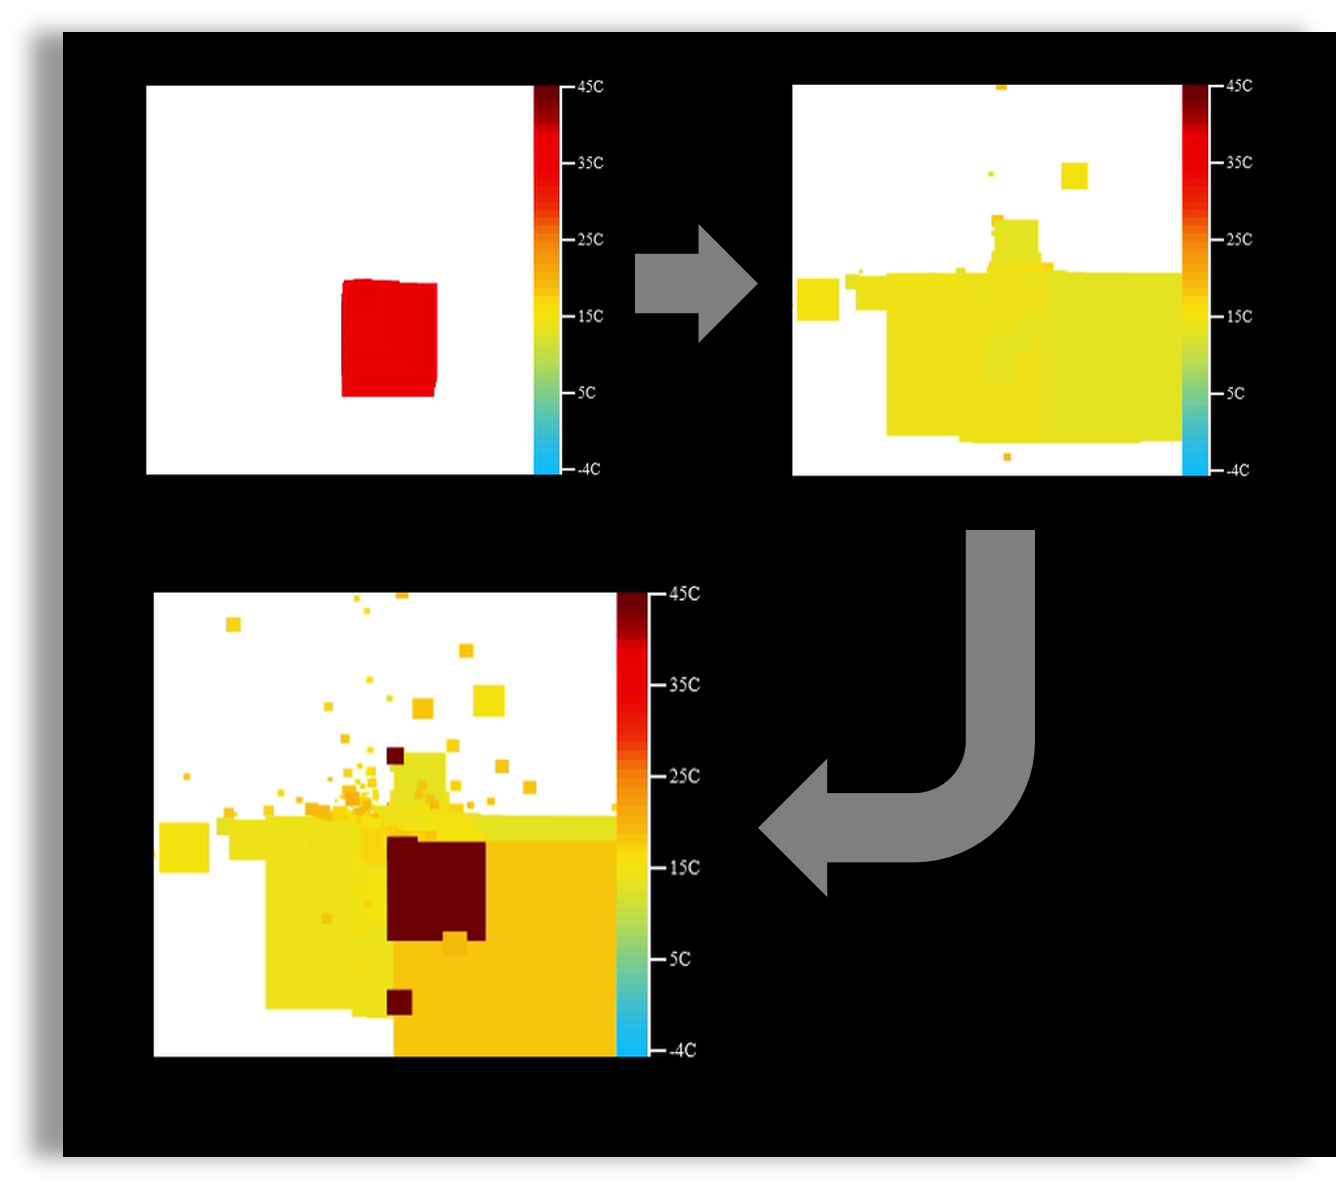
\includegraphics[scale=0.2]{tempmap.png}\hspace*{\fill}
		\caption{Temperature map buildup over the CanSat ascent and descent}
		\label{tempmap}
	\end{figure}

	The team believes the initial red square at approximately 35\degree C to represent the rocket engines below the CanSat, while the yellow squares represent the airfield, and can be seen at an approximately 17\degree C. The third image in figure \ref{tempmap} illustrates the combined image.
	
	Unfortunately, no positional tracking data was recovered.	
	
	\subsection{Module Status}
	
	Throughout the CanSat flight, landing, and time spent after impact, the CanSat experienced no hardware or sensor failures. Diagnostics conducted once a radio link was established confirmed that all sensors and devices on the CanSat were functional.
	
	The team believes this to be due to redundant and tough mechanical and electrical design.
	
	\chapter{Module Improvement}
	Despite the overall success of the team's final CanSat design, we believe that some substantial improvements can be made in all aspects of our design. Throughout the European competition the team noticed several major flaws in the final CanSat, distributed between mechanical design, electrical design, software design, and our base station design.	
	
	\section{Mechanical Design}
	Overall, the final CanSat's mechanical design was robust and lightweight, and therefore requires the fewest changes. The largest issue that the team noticed was that the use of a steel top frame as a vertical, conductive rod, near the antenna, created a dipole effect. This led to an unforeseen reduction in radio range as the internal frame absorbed part of the radio communication from our CanSat.
	
	Fortunately, this problem requires only minor design changes. By using a CanSat internal frame entirely constructed from 3D printed nylon, the CanSat would suffer no reduction in range. However, with this system the CanSat would still require additional mass: a conductive ring at the bottom of the CanSat, in between the outer shell and internal frame, could provide this mass. It's conductive qualities would also allow it to serve as ground plane: a feature recommended in our antenna specification list.
	
	\section{Electrical Design}
	Moving from our prototype to final CanSat, the team believes that the use of custom-manufactured printed circuit boards were a very positive design decision: they proved to be durable and allowed for higher component density than hand-wired perfboards. However, there is still room for improvement: implementing sensor integrated circuits directly on the PCB, instead of via breakout boards, would allow for even higher component density, providing room for more sensors to be implemented.
	
	It would also be worthwhile for the team to include an absolute orientation sensor \footnote{https://www.bosch-sensortec.com/bst/products/all\_products/bno055}, over raw accelerometers, gyroscopes, and magnetometers as seen in the Adafruit 9-DOF sensor used in the final CanSat \footnote{https://www.adafruit.com/product/1714}. Developing an accurate implementation of the Madgwick positional tracking algorithm proved to be a difficult and time-consuming task for the team, providing little benefit over pre-made solutions.
	
	The team experienced many issues with our GSM modem choice. The SIM800L, while inexpensive, only allowed for 2G network activation. Unfortunately, few cellular networks still support 2G activation, which made emergency GPS fallback impossible in the European competition. This can be fixed by replacing the SIM800L with a module such as the XBEE Cellular NB-IOT \footnote{https://www.digi.com/products/xbee-rf-solutions/embedded-cellular-modems/digi-xbee-cellular-nb-iot} would avoid this issue.
	
	Finally, the team experienced many issues with radio range over the two CanSat revisions. We believe that there are several causes to this issue:
	
	\begin{enumerate}
		\item \textbf{Lack of transmit power.} The XBEE 868LP radios operate a maximum transmit power of 25mW. This low transmit power, coupled with a relatively high baud rate of 9600 baud, led to issues with packet corruption. As a high baud rate is required for the large amount of information our secondary mission generates, our only radio-based recourse is transmitting at a higher power. \\
		\item \textbf{Antennae lacking directional properties.} While the Yagi antenna implemented in the final CanSat partially corrected this issue, the antenna only provided 11dBi gain. An antenna with more gain could serve to increase overall range. \\
		\item \textbf{Lack of radio availability over chosen bands.} The XBEE provides a robust set of native features, and allows for easy creation of mesh networks. However, few XBEE radios are certified for use in the European Union and provide the necessary radio range. It would be possible for the team to use a longer-range 433MHz radio and emulate mesh network features in software.
	\end{enumerate}
	
	There are many potential methods to increase radio range. The team proposes a two-pronged design shift as the most promising solution: pairing an 80kbps XBEE 868LP \footnote{https://www.digi.com/products/xbee-rf-solutions/sub-1-ghz-modules/xbee-868lp} with a long-range, low baud rate radio such as the Radiometrix NTX2 \footnote{http://www.radiometrix.com/content/ntx2}, with a cellular modem to provide emergency GPS location, would allow for long range, high baud rate, redundant communication.
	
	\section{Software Design}
	
	Overall, both CHIP Pro and Arduino software performed reliably. Despite this it is still possible to improve both aspects of the team's software work. The base station identified many packets as malformed, even if only a small number of characters were returned incorrectly: this led to large amounts of reported packet loss with a small amount of incorrect data. While it would reduce overall throughput due to an increased header/footer:data ratio, reducing packet sizes would lead to less overall data loss.
	
	While we experienced strong overall CHIP Pro performance for data processing, motion tracking, and temperature map creation applications, it would be possible to further increase performance by porting these specific algorithms into C++. However, this is not crucial for a successful secondary mission.
	
	\section{Base Station}
	
	The base station also performed without issue. Aside from the previously mentioned improvement of a higher gain antenna, it would be possible to make some quality-of-life changes with the base station user interface. These include:
	
	\begin{enumerate}
		\item \textbf{Add 3D CanSat orientation visualizer.} This functionality already existed in a separate demo written in Processing \footnote{https://processing.org/}. However, this functionality had never been incorporated into the base station proper. \\
		\item \textbf{Temperature map transparency.} Currently, temperature map data points overwrite any pre-existing pixels in the same location. Adding transparency would allow for easier visualization of average point temperature over multiple readings.
	\end{enumerate}
	
	
	\chapter{Outreach}
	Our team has taken a multifaceted approach to CanSat outreach, presenting at school events, events open to the public, and via websites and social media.
	\section{Online Presence}
	Our team has social media available on many platforms, including Facebook\footnote{https://www.facebook.com/cansatgwc}, Instagram\footnote{https://www.instagram.com/cansatgwc/}, and Twitter\footnote{https://twitter.com/cansatgwc2016}. Frequent updates and usage of social media tags allow us to draw people interested in our team and in the competition to our pages. We have and have planned to continue frequently updating our social media pages, through the entirety of the team's journey through the UK and EU competitions.
	
	The team has also designed a website to provide further online presence to our CanSat, to the CanSat competition, and to our sponsors. Our website is also frequently updated: a current snapshot can be seen in figure \ref{smedia}. 
	
	\begin{figure}
		\centering
		\begin{subfigure}{.5\textwidth}
			\centering
			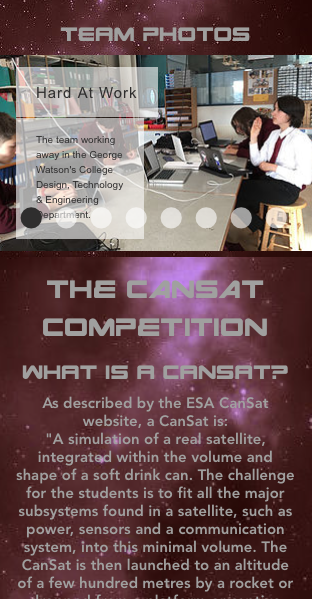
\includegraphics[width=.6\linewidth]{website.png}
		\end{subfigure}%
		\begin{subfigure}{.5\textwidth}
			\centering
			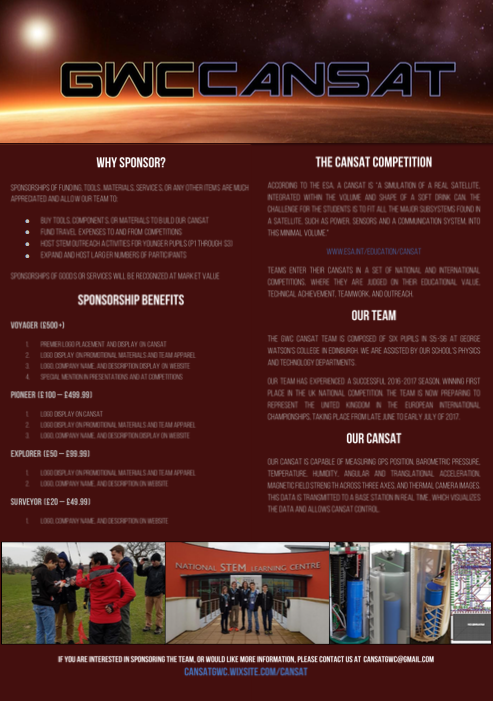
\includegraphics[width=0.8\linewidth, angle=0]{brochure.png}
		\end{subfigure}
		\caption{Various CanSat outreach materials}
		\label{smedia}
	\end{figure}
	
	The team has also created a sponsorship brochure for the upcoming season, which can be seen in figure \ref{smedia}.
	
	Our CanSat and team have also received substantial press, including articles on and in 3dprint.com\footnote{https://3dprint.com/175578/esa-cansat-competition-3d-print/}, tctmagazine.com\footnote{http://www.tctmagazine.com/3D-printing-news/croft-additive-manufacturing-provide-slm-3d-printed-casting-/}, stem.org.uk\footnote{https://www.stem.org.uk/esero/students-soar-success-space-competition}, Edinburgh Evening News \footnote{March 20th 2017}, @STEMLearningUK Twitter\footnote{https://twitter.com/STEMLearningUK/status/842463014397829122}, gwc.org.uk\footnote{https://www.gwc.org.uk/news/satellite-simulation-win-takes-team-to-european-finals/}, and @GWC\_News Twitter\footnote{https://twitter.com/GWC\_News/status/841582764491190272}.
	\section{In-Person Outreach}
	The team has also performed several in-person outreach events. We have run presentations in technology and physics for school open days, and have run full-school presentations to expand on our team and on the competition. In one full school presentation, we presented our success at the UK competition in the context of the successes and failures we experienced as a team new to the CanSat competition, explaining the difficulties we've faced and the solutions we've implemented to solve these issues.
	
	We have also initiated and ran educational outreach events for 9-10 year-old students. In the first session of the two-part workshop, students designed parachutes to meet certain descent velocity criteria: a reflection of the challenge we experienced in the UK CanSat competition. In the second section of the workshop, groups of students designed enclosure and padding to protect an egg dropped with their previously built parachute. To conclude the workshop, students tested their enclosure and parachute in a real-world egg drop. Some pictures of the event can be seen in figure \ref{eggdrop}.
	
	\begin{figure}
		\centering
		\begin{subfigure}{.5\textwidth}
			\centering
			\includegraphics[width=.8\linewidth]{ed1.jpg}
		\end{subfigure}%
		\begin{subfigure}{.5\textwidth}
			\centering
			\includegraphics[width=0.8\linewidth, angle=0]{ed2.jpg}
		\end{subfigure}
		\caption{Participants in the egg drop workshop}
		\label{eggdrop}
	\end{figure}
	
	Finally, the team presented in the Edinburgh Mini Maker Fair during the Edinburgh Science Festival. This gave the team the opportunity to present our progress within the competition as well as speak to other people interested in what we have been doing. This included a slideshow of pictures of the CanSat and the team's trip to York for the UK National Competition as well having a demonstration of the working CanSat, plotting data on graphs on a display. The team was also open to questions from the general public during the entirety of the Maker Faire. Our booth can be seen in figure \ref{mfair}.
	
	\begin{figure}[h]
		\hfill\includegraphics[scale=0.1]{mfaire.jpg}\hspace*{\fill}
		\caption{The team at Edinburgh Mini Maker Fair 2017}
		\label{mfair}
	\end{figure}
	
		
	\chapter{Team Information}
	
	\section{Team Management}
	
	\section{Team Organization and Roles}
	
	\begin{center}
		\begin{longtable}{rp{13cm}}		
			Team Member&Anna Lee \\
			Role&Teacher \\
			Background&Teacher of physics at George Watson's College \\
			Responsibilities&In charge of competing administrative paperwork for the team, and organizing travel\\
			\hline
			Team Member&Kaveh Pezeshki \\
			Role&Team Leader, Electronics Design and Assembly, Mechanical Design, Software Development \\
			Background&Key interests in physics, computer science, electrical and mechanical engineering, maths \\
			Responsibilities&Founded the team, communicated with sponsors and school administration and registered the team for the UK and EU competitions. Continued as a sponsor liaison and contact point for the team, as well as handling administrative tasks. Designed the overall system architecture, selected components, designed electrical layouts, and built the prototype cansat electronics board by hand. Assisted in component choice for the second revision, drew rough schematics, and prepared the completed PCBs. Brainstormed design ideas, drew CAD models of the CanSat design, and communicated with sponsors to build the prototype internal frame. Chose internal frame materials, and communicated with sponsors to create a complete physical 3D printed model of the internal frame. Used python to design and write the prototype CanSat and base station software, including packetization, independent data logging, multithreading, sensor control, and an interactive GUI.
			\\
			Time Committed&Approximately 500 hours out of school\\
			\hline
			Team Member&Calder Maclean \\
			Role&Software Development \\
			Background&Key interests in software and computer science \\
			Responsibilities&Programmed the CanSat module and onboard modules to read ambient humidity and temperature, GPS positioning, thermal imaging, etc. The CanSat stores raw data on board and transmits live data to the base station via a radio module\\
			Time Committed&Approximately 150 hours out of school\\
			\hline
			Team Member&Charles Cameron \\
			Role&Electronics design, mechanical assembly and outreach \\
			Background&Interested in physics, computer science, electrical and mechanical engineering, maths \\
			Responsibilities&CAD designed the PCB layout of electronic sub-systems using EAGLE for the second revision, as well as producing a bill of materials for the PCB assembly house. Liaison with sponsors and PCB manufacturers for assembly/implementation of a custom printed PCB. In charge of ordering team supplies and CanSat equipment, as well as keeping track of team expenses. Designed the GWC CanSat website and contributed to general outreach. Collaborated in constructing the CanSat outer shell.
			Prepared the prototype and final CanSat internal frames for implementation into the assembly \\
			Time Committed&Approximately 500 hours out of school\\
			\hline
			Team Member&Jack Hargreaves \\
			Role&Software Development \\
			Background&Key interests in software and computer science \\
			Responsibilities&Developed base station software to interpret incoming data from the CanSat which is then displayed in multiple graphs in real-time, as well as being stored onboard. In addition, the status of all sensors is displayed in a visual representation of the CanSat.\\
			Time Committed&Approximately 200 hours out of school\\
			\hline
			Team Member&Pedro Guimaraes \\
			Role&Mechanical Design \\
			Background&Key interests in computer science, maths, and chemistry \\
			Responsibilities&Designed and constructed prototypes for the CanSat outer shell. Brainstormed and constructed prototypes for test fixture release mechanisms for the CanSat.\\
			Time Committed&Approximately 100 hours out of school\\
			\hline
			Team Member&Morven Pennie \\
			Role&Outreach Representative, Mechanical Design, Graphical Designer \\
			Background&Key interests in computer science, graphic design, mechanical engineering and art \\
			Responsibilities&Brainstormed and designed team graphics for the team website, social media and public events, such as the Edinburgh Mini Maker Faire. Designed and coordinated team apparel and CanSat external graphics. Collaborated in constructing the CanSat outer shell. Lead social media representative for the team, including taking/gathering promotional photos. Animated the CanSat logo for promotional videos in addition to editing the team videos.\\
			Time Committed&Approximately 400 hours out of school\\
		\end{longtable}
	\end{center}
	
\end{document}